% Írta: Halmos Balázs Paszkál
\documentclass[12pt,a4paper]{article}
\usepackage[utf8]{inputenc}
\usepackage[magyar]{babel}
\usepackage[T1]{fontenc}
\usepackage{amsmath}
\usepackage{amsfonts}
\usepackage{amssymb}
\usepackage[left=2cm,right=2cm,top=2cm,bottom=2cm]{geometry}
\usepackage{amsthm} % A bizonyításhoz
\author{Halmos Balázs}
\date{2022/2023}
\title{Matematika érettségi tételek}

\usepackage{enumitem} % Római számozás a listákhoz

% Létrehozza a definició és a tétel környezeteket
\newtheorem{theorem}{Tétel} [section]
\newtheorem{definition}{Definíció} [section]

% A kattintható tartalomjegyzékhez
\usepackage{hyperref}
\hypersetup{
    colorlinks,
    citecolor=black,
    filecolor=black,
    linkcolor=black,
    urlcolor=black
}
% A kép beillesztéséhez
\usepackage{graphicx}
\graphicspath{ {./img/} }
\usepackage{wrapfig}

\usepackage{array} %
\DeclareMathOperator{\tg}{tg}
\DeclareMathOperator{\ctg}{ctg}
\DeclareMathOperator{\arctg}{arctg}

% Hogy jobb oldali casest lehessen használni
\newenvironment{rcases}
  {\left.\begin{aligned}}
  {\end{aligned}\right\rbrace}

\begin{document}
\maketitle
\tableofcontents
\newpage
\section{Halmazok, halmazműveletek. Nevezetes ponthalmazok a síkban és a térben}

\subsection{Halmazok, részhalmazok}

\textbf{A halmaz és a halmaz eleme alapfogalom}, ezeket a kifejezéseket nem definiáljuk. De a halmaz megadásának szigorú követelménye van: egy halmazt úgy kell megadnunk, hogy minden szóba jöhető dologról egyértelműen eldönthető legyen, hogy az adott halmazhoz tartozik vagy sem. A halmazokat nyomtatott nagybetűvel, a halmaz elemeit kisbetűvel jelöljük a következő módon:

$A=\{a;b;c\}$, ebben az esetben: $a\in A, x\notin A$

\vspace{20px}
\textbf{Halmaz megadási módjai:}
\begin{itemize}
\item  Elemeinek felsorolásával: $A = \{0; 2; 4; 6\}$
\item  Az elemeit egyértelműen meghatározó utasítással: $B = \{$egyjegyű páratlan számok$\}$
\item Szimbólumokkal: $A=\{x|x^2-x-6=0\}, B=\{x|x^2>9\}$
\item Venn-diagrammal:
\begin{figure}[h]
\centering
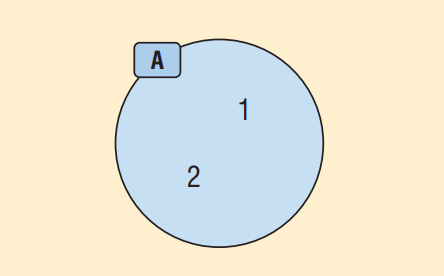
\includegraphics[scale=0.3]{img/venn_diagram}
\end{figure}
\end{itemize}

\begin{definition}
\textbf{Két halmaz egyenlő}, ha ugyanazokat az elemeket tartalmazzák.
\end{definition}

\begin{definition}
Az elem nélküli halmazt \textbf{üres halmaz}nak nevezzük.

Jele: $\{ \}$ vagy $\varnothing$ 
\end{definition}

\begin{definition}
Az A halmaz \textbf{részhalmaz}a a B halmaznak, ha A minden eleme a B halmaznak is eleme.

Jele: $A\subseteq B$
\end{definition}

\begin{definition}
Az A halmaz \textbf{valódi részhalmaz}a a B halmaznak, ha A részhalmaza a B-nek, de nem egyenlő vele.

Jele: $A\subset B$
\end{definition}

Tulajdonságok:
\begin{itemize}
\item Az üres halmaz minden halmaznak részhalmaza: $\varnothing \subseteq A$.
\item Minden halmaz önmaga részhalmaza: $A\subseteq A$.
\item Ha $A\subseteq B$ és $B\subseteq A$, akkor $A=B$.
\item Ha $A\subseteq B$ és $B\subseteq C$, akkor $A\subseteq C$. 
\end{itemize}
\newpage
\begin{theorem}
\textbf{Az ``n'' elemű halmaz összes részhalmazainak száma: $2^n (n\in \mathbb{N})$}
\end{theorem}
\begin{proof}
A bizonyítást teljes indukcióval végezzük, amelynek lényege, hogy először belátjuk egy konkrét $n$ esetére az állítást, majd azt mutatjuk meg, ha az állítás igaz egy tetszőleges $n$-re, akkor igaz az őt követő $(n + 1)$-re is, azaz bizonyítjuk az állítás öröklődését.

Az üres halmaznak egyetlen részhalmaza van: önmaga $(2^0 = 1)$.

Egy egyelemű halmaznak 2 részhalmaza van: az üres halmaz és önmaga $(2^1 = 2)$

Egy kételemű halmaznak 4 részhalmaza van: az üres halmaz, 2 egyelemű halmaz és önmaga $(2^2 = 4)$.

Tegyük fel, hogy egy $k$ elemű halmaznak $2^k$ db részhalmaza van. Bizonyítani kell, hogy ez öröklődik, vagyis egy $(k + 1)$ elemű halmaznak $2^{k + 1}$ db részhalmaza van.

Tekintsük az előbbi $k$ elemű halmazt. Ekkor ha az eddigi elemek mellé egy $(k + 1)$-edik elemet teszünk a halmazba, akkor ezzel megkétszerezzük a lehetséges részhalmazok számát, hiszen az új elemet vagy kiválasztjuk az eddigi részhalmazokba, vagy nem. Vagyis a $(k + 1)$ elemű halmaz részhalmazainak száma $2 \cdot 2^k = 2^{k + 1}$, amit bizonyítani kívántunk.
\end{proof}

\subsection{Halmazműveletek}

\begin{definition}
Azt a halmazt, amelynek a vizsgált halmazok részhalmazai, \textbf{alaphalmaz}nak vagy univerzumnak nevezzük.

Jele: ``U'' vagy ``H''.
\end{definition}

\begin{definition}
Egy ``A'' halmaz \textbf{komplementer halmaz}ának az alaphalmaz azon elemeinek halmazát nevezzük, amelyek az A halmaznak nem elemei. Jele: $\overline{A}$. (Fontos tulajdonság: $\overline{\overline{A}} = A$.)
\end{definition}

\begin{definition}
Két vagy több halmaz \textbf{unió}ja vagy egyesítése mindazon elemek halmaza, amelyek legalább az egyik halmaznak elemei. Jele: $\cup$.
\end{definition}

\begin{definition}
Két vagy több halmaz \textbf{metszet}e vagy közös része pontosan azoknak az elemeknek a halmaza, amelyek mindegyik halmaznak elemei. Jele: $\cap$.
\end{definition}

\begin{definition}
Két halmaz \textbf{diszjunkt}, ha nincs közös elemük, vagyis a metszetük üres halmaz.

$A\cap B=\varnothing$.
\end{definition}

\begin{definition}
Az ``A'' és ``B'' halmaz \textbf{különbsége} az A halmaz mindazon elemeinek halmaza, amelyek a B halmaznak nem elemei. Jele: $A \setminus B$.
\end{definition}

\begin{definition}
Az ``A'' és ``B'' halmaz \textbf{Descartes-féle szorzata} az a halmaz, amelynek elemei az összes olyan rendezett $(a; b)$ pár, amelynél $a\in A$ és $b\in B$. Jele: $A\times B$.
\end{definition}

\begin{figure}[h]
\centering
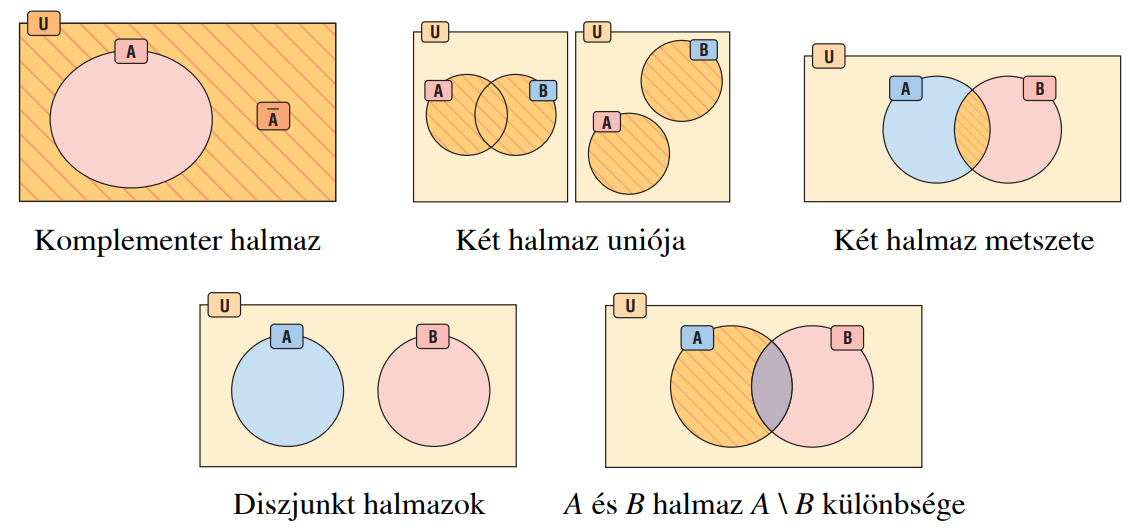
\includegraphics[scale=0.29]{img/halmazok}
\end{figure}
\newpage
\textbf{Halmazműveletek tulajdonságai}

\begin{figure}[h]
\centering
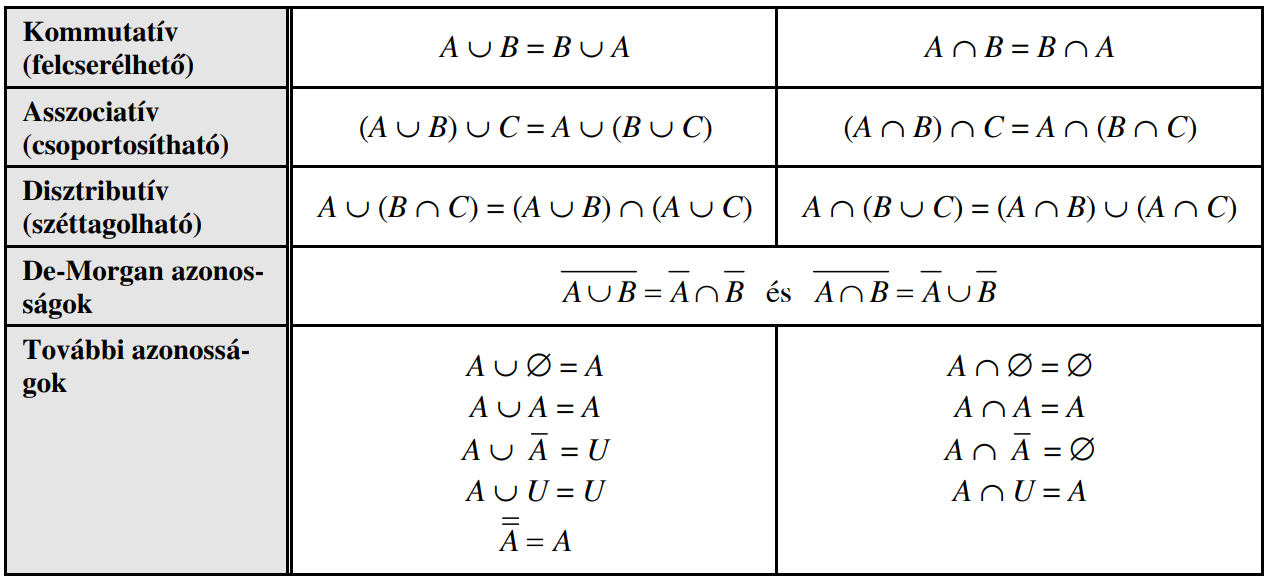
\includegraphics[scale=0.35]{img/halmazmuveletek}
\end{figure}

\subsection{Nevezetes ponthalmazok a síkban és a térben}

\begin{definition}
Azoknak a pontoknak a halmaza a síkon, amelyek a sík egy adott ``O'' pontjától adott ``r'' távolságra vannak, egy ``O'' középpontú, ``r'' sugarú \textbf{kör}.
\end{definition}

\begin{definition}
Azoknak a pontoknak a halmaza a térben, amelyek a tér adott ``O'' pontjától adott ``r'' távolságra vannak, egy ``O'' középpontú, ``r'' sugarú \textbf{gömb}.
\end{definition}

\begin{definition}
Adott egyenestől adott távolságra lévő pontok halmaza a síkon az egyenessel \textbf{párhuzamos egyenespár}.
\end{definition}

\begin{definition}
Adott egyenestől adott távolságra lévő pontok halmaza a térben olyan \textbf{hengerfelület}, amelynek tengelye az adott egyenes.
\end{definition}

\begin{definition}
Két ponttól egyenlő távolságra lévő pontok halmaza a síkban a \textbf{szakasz felezőmerőleges egyenese}.
\begin{figure}[h]
\centering
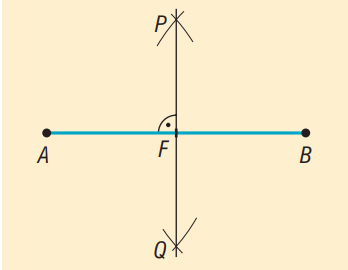
\includegraphics[scale=0.35]{img/szakaszfelezo_meroleges}
\end{figure}
\end{definition}
\newpage
\begin{definition}
Két ponttól egyenlő távolságra lévő pontok halmaza a térben a \textbf{szakasz felezőmerőleges síkja}.
\begin{figure}[h]
\centering
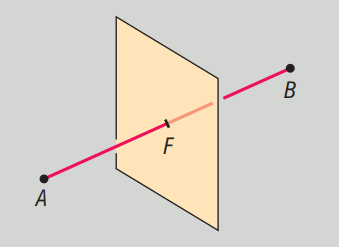
\includegraphics[scale=0.35]{img/szakaszfelezo_meroleges_sik}
\end{figure}
\end{definition}

\begin{definition}
Két párhuzamos egyenestől egyenlő távolságra lévő pontok halmaza a síkban olyan egyenes, amely a két adott egyenessel párhuzamos és távolságukat felezi (\textbf{középpárhuzamos}).
\end{definition}

\begin{definition}
Két metsző egyenestől egyenlő távolságra lévő pontok halmaza az általuk bezárt szögek \textbf{szögfelező egyenesei}. Két ilyen egyenes van, ezek merőlegesek egymásra.
\begin{figure}[h]
\centering
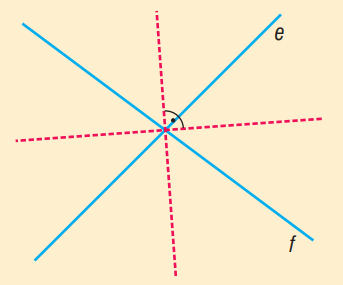
\includegraphics[scale=0.35]{img/szogfelezo_egyenes}
\end{figure}
\end{definition}

\begin{definition}
Egy egyenestől és egy rajta kívül lévő ponttól egyenlő távolságra lévő pontok halmaza a síkon: a \textbf{parabola}.

Az adott pont a parabola fókuszpontja, az adott egyenes a parabola vezéregyenese (direktrixe), a pont és az egyenes távolsága a parabola paramétere.
\begin{figure}[h]
\centering
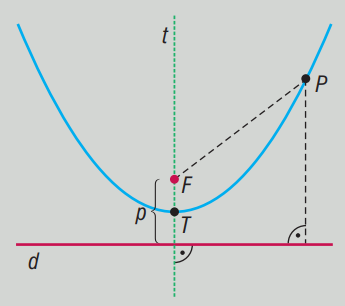
\includegraphics[scale=0.35]{img/parabola}
\end{figure}
\end{definition}

\subsection{Egyéb ponthalmazok}
\begin{definition}
Azoknak a pontoknak a halmaza a síkon, amelyeknek a sík két különböző adott pontjától mért távolságösszege az adott pontok távolságánál nagyobb állandó: \textbf{ellipszis}.

A két adott pont $(F_1$ és $F_2)$ az ellipszis fókuszpontjai. Az adott távolság az ellipszis nagytengelye, az $F_1F_2$ szakasz felezőmerőlegesének az ellipszis tartományába eső szakasza az ellipszis kistengelye.
\end{definition}

\begin{definition}
Azoknak a pontoknak a halmaza a síkon, amelyeknek a sík két különböző adott pontjától mért távolságkülönbségének abszolút értéke a két adott pont távolságánál kisebb állandó: \textbf{hiperbola}.

A két adott pont $(F_1$ és $F_2)$ a hiperbola fókuszpontjai, az adott távolság a hiperbola főtengelye.
\end{definition}

\begin{theorem}
Három adott ponttól egyenlő távolságra lévő pontok halmaza a síkon egy pont (ha a 3 pont nem esik egy egyenesre), vagy üres halmaz (ha a 3 pont egy egyenesre esik).
\begin{figure}[h]
\centering
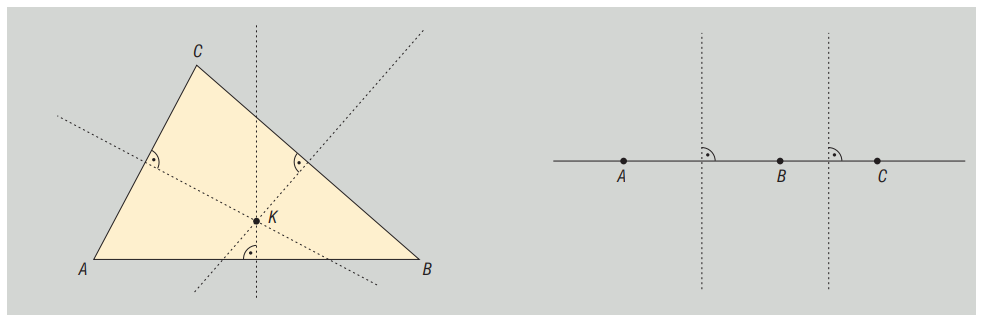
\includegraphics[scale=0.35]{img/haromszog_harom_pont}
\end{figure}
\end{theorem}

\begin{theorem}
A háromszög három oldalfelező merőlegese egy pontban metszi egymást.
\end{theorem}

\begin{theorem}
A háromszög oldalfelező merőlegeseinek metszéspontja a \textbf{háromszög köré írt kör középpontja}.
\end{theorem}

A háromszög köré írt kör középpontja hegyesszögű háromszög esetén a háromszögön belül, derékszögű háromszögnél az átfogó felezőpontjába (Thalész tétele), tompaszögű háromszögnél a háromszögön kívül esik.
\begin{figure}[h]
\centering
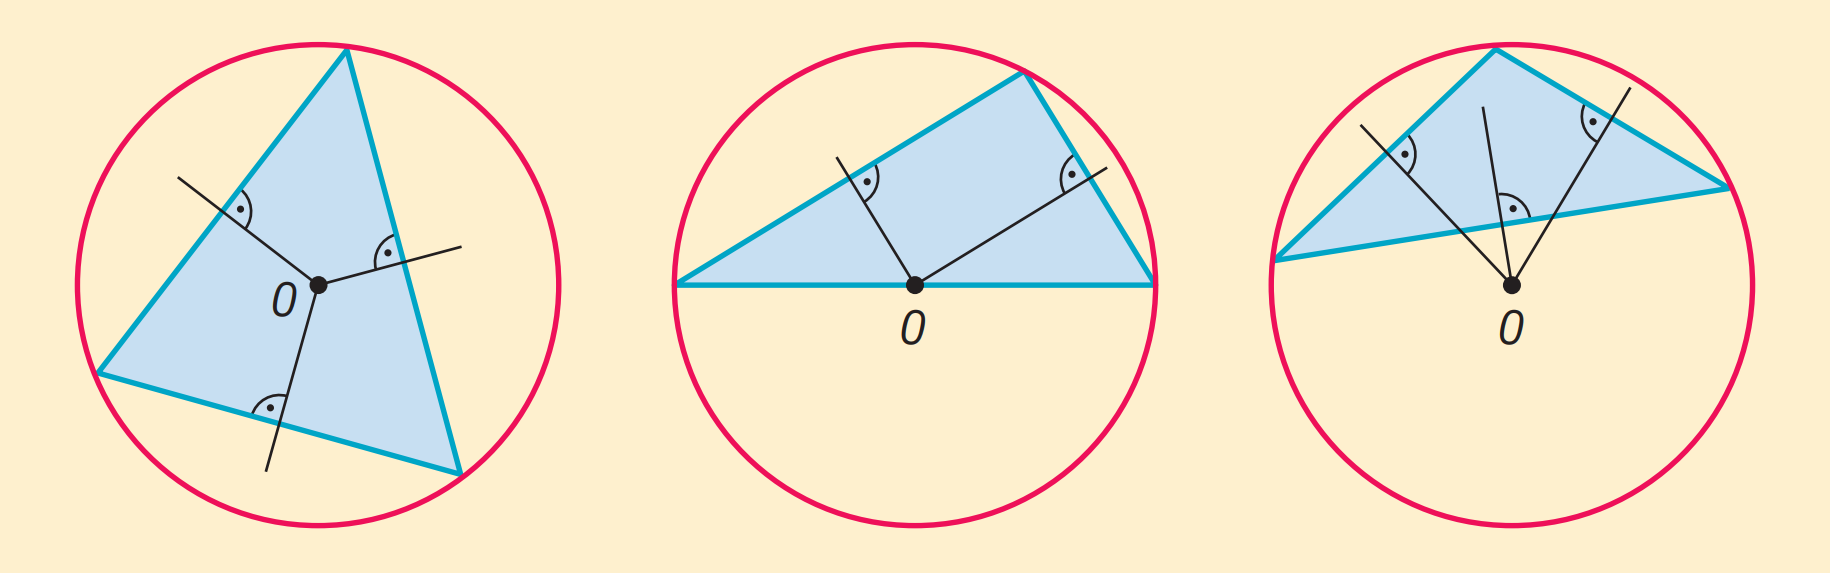
\includegraphics[scale=0.2]{geometry/korul_irt_kor_esetek}
\end{figure}

\begin{theorem}
Három adott ponttól egyenlő távolságra lévő pontok halmaza a térben egy olyan egyenes, amely áthalad a három pont, mint háromszög köré írható kör középpontján, és merőleges a 3 pont síkjára (ha a 3 pont nem esik egy egyenesbe), vagy üres halmaz (ha a 3 pont egy egyenesbe esik).
\end{theorem}
\newpage
\begin{theorem}
Három egyenestől egyenlő távolságra lévő pontok halmaza a síkon:
\begin{itemize}
\item Ha a 3 egyenes párhuzamos, akkor üres halmaz.
\item Ha 2 egyenes párhuzamos $(e || f)$, egy pedig metszi őket $(g)$, akkor a 2 párhuzamos egyenes középpárhuzamosán két olyan pont, amelyek illeszkednek két metsző egyenes (pl. ``e'' és ``g'') szögfelezőire.
\begin{figure}[h]
\centering
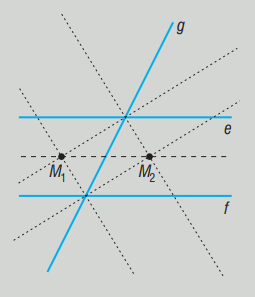
\includegraphics[scale=0.4]{img/harom_egyenes_1}
\end{figure}
\item  Ha a 3 egyenes 3 különböző pontban metszi egymást, akkor szögfelező egyeneseik metszéspontjai. 4 ilyen pont van, az egyik a \textbf{háromszög beírt körének}, 3 pedig a \textbf{háromszög hozzáírt köreinek} középpontja.
\begin{figure}[h]
\centering
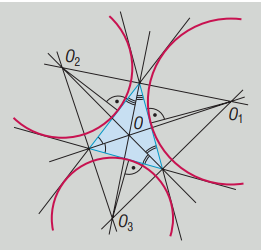
\includegraphics[scale=0.4]{img/harom_egyenes_2}
\end{figure}
\item  Ha a 3 egyenes egy pontban metszi egymást, akkor egyetlen pont, a 3 egyenes metszéspontja.
\begin{figure}[h]
\centering
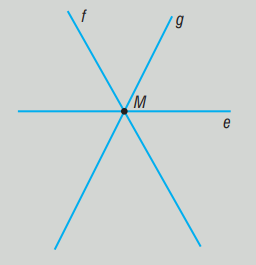
\includegraphics[scale=0.4]{img/harom_egyenes_3}
\end{figure}
\end{itemize}
\end{theorem}
\newpage
\begin{definition}
Azon pontok halmaza amelyekből a sík egy AB szakasza adott $\alpha (0^\circ < \alpha < 180^\circ)$ szög alatt látszik, két, az AB egyenesre szimmetrikusan elhelyezhető körív, melynek neve az AB szakasz $\alpha$ szögű \textbf{látókörív}e. A szakasz két végpontja nem tartozik a ponthalmazba.
\end{definition}
\begin{figure}[h]
\centering
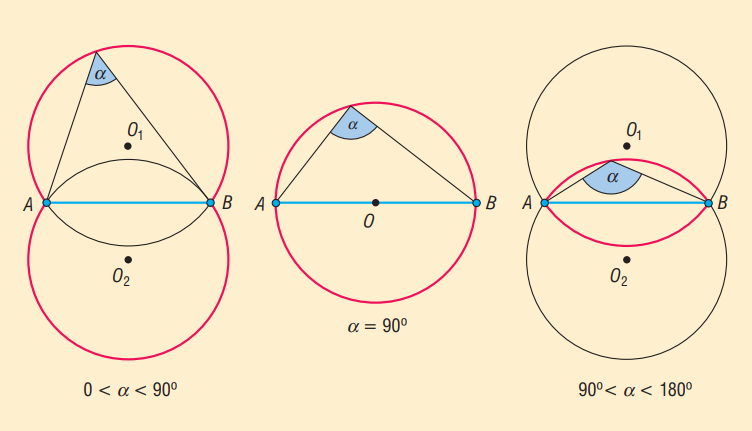
\includegraphics[scale=0.3]{geometry/latorkoriv}
\end{figure}
\subsection{Alkalmazások}
\begin{itemize}
\item Biológiában a rendszertan, kémiában a periódusos rendszerbeli csoportosítás is halmazelméleti fogalmak. Műveletek: melyik csoport melyiknek részhalmaza?
\item  Vércsoport szerint az emberek különböző halmazokba sorolhatók. Műveletek: ki kinek adhat vért?
\item Európa országai hivatalos nyelvük alapján halmazokba sorolhatók. Műveletek: melyik országban hivatalos nyelv az angol vagy a német?
\item  Az érettségin a nem kötelező tárgyak választása szerint is halmazokba sorolhatók a vizsgázók. Műveletek: ki vizsgázik kémiából és biológiából is?
\item  A függvényekkel kapcsolatban is használjuk a halmazokat (értelmezési tartomány, értékkészlet).
\item Egyenletek értelmezési tartományának vizsgálatakor számhalmazok metszetét képezzük.
\item Koordináta-geometriában a kör, a parabola, az ellipszis és a hiperbola egyenletének felírásakor az adott görbe definícióját használjuk fel.
\item Látókörívek: egy téglalap egyik oldala a szomszédos oldal mely pontjából látszik a legnagyobb szögben (színház, sportpálya).
\item Szerkesztési feladatokban: háromszög szerkesztése egy oldal, a vele szemközti szög és az oldalhoz tartozó magasság ismeretében, vagy adott. egy pont és egy egyenes, szerkesszük meg az egyenest érintő, a ponton áthaladó, adott sugarú köröket.
\item Parabolaantennák.
\item Két tanya közös postaládát kap az országút mentén. Hova helyezzék, hogy mindkét tanyától egyenlő távolságra legyen?
\begin{figure}[h]
\centering
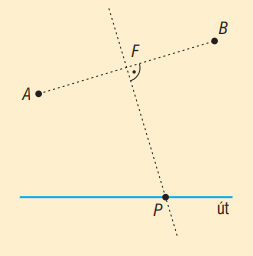
\includegraphics[scale=0.2]{img/postaladak_helye}
\end{figure}
\end{itemize}

\newpage


\section{Racionális és irracionális számok. Műveletek a racionális és irracionális számok halmazán. Közönséges és tizedes törtek. Halmazok számossága}

\subsection{Számhalmazok}

\begin{definition}
A \textbf{természetes számok} halmaza $(\mathbb{N})$ a pozitív egész számokból és a 0-ból áll.

A természetes számok halmaza zárt az összeadásra és a szorzásra nézve, azaz bármely két természetes szám összege és szorzata természetes szám. Ugyanakkor a kivonás és az osztás már nem végezhető el ezen a halmazon belül, ezek a műveletek „kimutatnak” a halmazból.

Pl. $3 - x = 5$ egyenlet megoldása.
\end{definition}

\begin{definition}
Az \textbf{egész számok} halmaza $(\mathbb{Z})$ a természetes számokból és azok ellentettjeiből áll. Az egész számok halmaza az összeadáson és a szorzáson kívül a kivonásra nézve is zárt, ugyanakkor az osztás kimutathat a halmazból. Pl. $2x + 3 = 4$ egyenlet megoldása.
\end{definition}

\begin{definition}
A \textbf{racionális számok} halmaza $(\mathbb{Q})$ azokból a számokból áll, amelyek felírhatók két egész szám hányadosaként, azaz $\dfrac{a}{b}$ alakban, ahol $a, b\in \mathbb{Z}, b \neq 0$.

A racionális számok halmaza mind a 4 alapműveletre zárt (osztásra, ha az osztó nem 0), de itt is találunk olyan egyenletet, amelynek nincs megoldása ezen a halmazon. Pl.: $2x^2 - 3 = 0$.
\end{definition}

\begin{definition}
Azokat a számokat, amelyek nem írhatók fel két egész szám hányadosaként, \textbf{irracionális számoknak} $(\mathbb{Q}^*)$ nevezzük.
\end{definition}

\begin{theorem}
$\sqrt{2}$ irracionális szám.
\end{theorem}
\begin{proof}
A bizonyítást indirekt módon végezzük, lényege, hogy a bizonyítandó állítás tagadásáról bebizonyítjuk, hogy az hamis. Ez azt jelenti, hogy a bizonyítandó állítás igaz.

Tegyük fel hogy $\sqrt{2}$ racionális szám, azaz felírható $\dfrac{a}{b}$ alakban, ahol $a, b\in \mathbb{Z}, b \neq 0,$ és $(a; b)=1$.

Ekkor: $\sqrt{2}=\dfrac{a}{b}\Rightarrow 2= \dfrac{a^2}{b^2}\Rightarrow 2\cdot b^2=a^2$.

Az egyenlet jobb oldalán szereplő $(a^2)$ szám prímtényezős felbontásában a 2 mindenféleképpen páros kitevőn (akár a nulladikon) szerepel, míg a bal oldalon levő szám $(2 \cdot b^2)$ prímtényezős felbontásában a 2 kitevője páratlan (legkevesebb 1).

Ez azonban lehetetlen, hiszen a számelmélet alaptétele szerint egy pozitív egész számnak nincs két lényegesen különböző felbontása.

Tehát nem igaz az indirekt feltevésünk, vagyis igaz az eredeti állítás: $\sqrt{2}$ irracionális.
\end{proof}

Tulajdonságok:
\begin{itemize}
\item Az irracionális számok halmaza nem zárt a 4 alapműveletre $\left(\sqrt{2} + \left(-\sqrt{2}\right) \right)=0\notin \mathbb{Q}^*$, $\sqrt{2} \cdot \sqrt{2}=2\notin \mathbb{Q}^*$,$\sqrt{2} : \sqrt{2}=1\notin \mathbb{Q}^*$
\item Az irracionális számok tizedes tört alakja végtelen nem szakaszos tizedes tört.
\end{itemize}
\newpage
\begin{definition}
A racionális és az irracionális számok halmaza diszjunkt halmazok $(\mathbb{Q} \cap \mathbb{Q}^*=\varnothing)$, a két halmaz egyesítése a valós számok halmaza: $\mathbb{R}=\mathbb{Q} \cup \mathbb{Q}^*$
A valós számok halmaza zárt a 4 alapműveletre.
A valós számok és részhalmazai:
\begin{figure}[h]
\centering
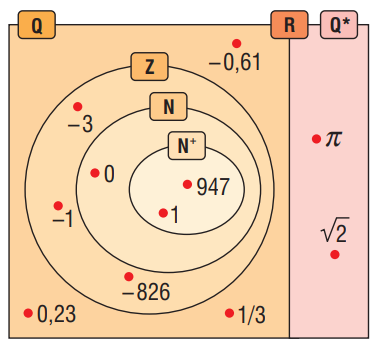
\includegraphics[scale=0.3]{img/szam_halmazok}
\end{figure}
\end{definition}

\subsection{Műveletek a racionális számok halmazán}
Egy közönséges tört értéke nem, csak az alakja változik, ha a számlálóját és a nevezőjét ugyanazzal a 0-tól különböző számmal szorozzuk (bővítés), vagy ugyanazzal a 0-tól különböző számmal osztjuk (egyszerűsítés).
Ha a racionális számok közönséges tört alakúak, akkor a következő szabályokkal lehet elvégezni az alapműveleteket:
\begin{itemize}
\item \textbf{Összeadás és kivonás:}

Csak azonos nevezőjű törteket lehet összeadni, kivonni, ezért a törteket bővítjük egy közös többszörösű nevezőre (legjobb, ha a legkisebb közös többszörösű nevezőre, mert így tudunk a legkisebb számokkal számolni):
$$\dfrac{a}{b}\pm\dfrac{c}{d}=\dfrac{a\cdot d}{b\cdot d}\pm\dfrac{c\cdot b}{d\cdot b}=\dfrac{a\cdot d \pm c\cdot b}{b\cdot d}\hspace{20px} b,d\neq 0$$
Ha a nevezők $(b$ és $d)$ relatív prímek, akkor a legkisebb közös többszörösük a szorzatuk.
\item \textbf{Szorzás:}

Törtet törttel úgy szorzunk, hogy a számlálót a számlálóval, nevezőt a nevezővel szorozzuk:
$$\dfrac{a}{b}\cdot\dfrac{c}{d}=\dfrac{a\cdot c}{b\cdot d}\hspace{20px} b,d\neq 0$$
Egész számmal úgy szorzunk törtet, hogy törtként írjuk fel a szorzót $\left(c=\dfrac{c}{1} \right)$, vagyis igazából a számlálót megszorozzuk, a nevezőt változatlanul hagyjuk.
\item \textbf{Osztás:}

Törtet törttel úgy osztunk, hogy a változatlan osztandót szorozzuk az osztó reciprokával:
$$\dfrac{a}{b}:\dfrac{c}{d}=\dfrac{a}{b}\cdot\dfrac{d}{c}=\dfrac{a\cdot d}{b\cdot c}\hspace{20px} b,c,d\neq 0$$
Egész számmal úgy osztunk, hogy törtként írjuk fel az osztót $\left(c=\dfrac{c}{1} \right)$, vagyis igazából a nevezőt megszorozzuk, a számlálót változatlanul hagyjuk, vagy (egyszerűsíthető esetben) a számlálót osztjuk, a nevezőt változatlanul hagyjuk.
\end{itemize}
\newpage
\subsection{Műveletek az irracionális számok halmazán}
Az alapműveletek definiálhatók az irracionális számok körében úgy, hogy az eddigi azonosságok életben maradjanak. Mivel tizedes tört alakjuk végtelen, nem periodikus, így azt csak közelítően tudjuk megadni. Ezért a pontos értékeket pl. hatvány, gyök, logaritmus alakban adjuk meg, ilyenkor viszont a megfelelő műveleti szabályokkal dolgozunk.
\subsection{Műveleti tulajdonságok $a, b, c \in \mathbb{R}$ esetén}
\begin{enumerate}
\item az összeadás és a szorzás kommutatív (felcserélhető)
$$a+b=b+a\text{ és } a\cdot b=b\cdot a$$
\item az összeadás és a szorzás asszociatív (csoportosítható)
$$(a+b)+c=a+(b+a) \text{ és } (a\cdot b)\cdot c=a\cdot (b\cdot a)$$
\item a szorzás az összeadásra nézve disztributív (széttagolható)
$$(a+b)\cdot c=a\cdot c+b\cdot c$$
\end{enumerate}
\subsection{Közönséges és tizedes törtek}
A közönséges törtek formái lehetnek:
Az $\dfrac{a}{b}$ közönséges tört, vagyis az $\dfrac{a}{b}$ hányados a következő alakokban fordulhat elő ($a, b \in \mathbb{Z}, b \neq 0$, és a tört végsőkig leegyszerűsített, azaz $a$ és $b$ legnagyobb közös osztója 1):
\begin{itemize}
\item egész szám, ha $b$ osztója $a$-nak,
\item  véges tizedes tört, ha $b$ prímtényezős felbontásában a 2 és az 5 számokon kívül nincs más prímszám,
\item végtelen szakaszos tizedes tört, ha $b$ prímtényezős felbontásában a 2 és az 5 számokon kívül más prímszám is van.
\end{itemize}
Tehát a racionális számok a következő alakúak: közönséges törtek, egészek, véges vagy végtelen szakaszos tizedes törtek.

\textbf{A tizedes törtek formái lehetnek:}
\begin{itemize}
\item véges tizedes törtek, ezek felírhatók közönséges tört alakban. Pl. $2,3=\dfrac{23}{10}$.
\item végtelen tizedes törtek:
\begin{itemize}
\item szakaszos tizedes törtek, ezek felírhatók közönséges tört alakban. Pl. végtelen mértani sor összegeként, vagy a következő módszerrel:
\begin{align*}
2,354545...&=x \\
235,454545...&=100x
\end{align*}
A két egyenletet kivonva egymásból
$$233,1=99x\Rightarrow x=\dfrac{233,1}{99}=\dfrac{2331}{990}$$
\item  nem szakaszos tizedes törtek \textbf{nem} írhatóak át közönséges tört alakba.
\end{itemize}
\end{itemize}


\textbf{Összefoglalva:}
A közönséges törtek mind felírhatók tizedes tört alakban (egész, véges, végtelen szakaszos tört alakban).

A nem szakaszos tizedes törtek mind irracionális számok, tehát nem írhatók fel két egész szám hányadosaként, tehát nem közönséges törtek. Ebből következik, hogy nem minden tizedes tört közönséges tört.

\subsection{Halmazok számossága}
\begin{definition}
Egy ``A'' \textbf{halmaz számossága} az ``A'' halmaz elemeinek számát jelenti. Jele: $|A|$. Egy halmaz számossága lehet véges vagy végtelen.
\end{definition}

\begin{definition}
Egy halmaz \textbf{véges halmaz}, ha elemeinek számát egy természetes számmal megadhatjuk. Ellenkező esetben, azaz ha a halmaz elemeinek számát nem adhatjuk meg természetes számmal, akkor \textbf{végtelen halmaz}ról beszélünk.
\end{definition}

\begin{definition}
A végtelen halmazok között találhatunk olyat, melynek elemei sorba rendezhetők, tehát megadható az 1., 2., 3., 4., … eleme. A pozitív természetes számokkal megegyező számosságú halmazokat \textbf{megszámlálhatóan végtelen halmazoknak} nevezzük.

A megszámlálhatóság és a sorba rendezhetőség egy végtelen halmaznál ugyanazt jelenti.

Minden olyan halmaz megszámlálhatóan végtelen számosságú, amelynek elemei és a természetes számok között kölcsönösen egyértelmű megfeleltetés létesíthető.

Megszámlálhatóan végtelen számosságúak: egész számok, páros számok, négyzetszámok, racionális számok.
\end{definition}

\begin{definition}
A valós számok számosságával megegyező számosságú halmazokat \textbf{nem megszámlálhatóan végtelen} vagy kontinuum számosságú halmazoknak nevezzük. Pl.: irracionális számok halmaza, számegyenes pontjainak halmaza, intervallum pontjainak halmaza.
\end{definition}

\begin{theorem}
Számosság és halmazműveletek kapcsolata (logikai szita): A, B és C véges halmazok számosságára érvényesek a következők:
$$|A\cup B| = |A| + |B|- |A\cap B|$$
$$\left|\overline{A\cup B}\right|=|U|-|A\cup B|$$
$$|A\cup B\cup C|=|A|+|B|+|C|-|A\cap B|-|A\cap C|-|B\cap C|+|A\cap B\cap C|$$
\end{theorem}
\subsection{Alkalmazások}
\begin{itemize}
\item Racionális számok: arányok, arányosság, hasonlóság
\item Irracionális számok: szabályos háromszög magassága $\left(\dfrac{a\sqrt{3}}{2} \right)$, négyzet átlója: $a\sqrt{2}$, köt kerülete: $2r\pi$, területe: $r^2\pi$
\item Kifejezések legbővebb értelmezési tartományának meghatározása, pl: $\sqrt{x+2}+\dfrac{1}{\sqrt{2-x}}$
\item Függvény értékkészletének megállapítása
\end{itemize}
\newpage


\section{Oszthatóság, oszthatósági szabályok és tételek. Prímszámok. Számrendszerek}
\subsection{Oszthatóság}
Az oszthatóság fogalmánál alaphalmaznak az egész számok halmazát tekintjük. Két egész szám hányadosa nem mindig egész szám, az oszthatóságnál azt vizsgáljuk, hogy egész számok osztásakor mikor lesz a hányados is egész szám, vagyis a maradék 0.

\begin{definition}
Egy ``a'' egész szám \textbf{osztó}ja egy ``b'' egész számnak, ha található olyan ``c'' egész szám, amelyre $a \cdot c = b$. Jelölés: $a|b$. (Természetesen $c|b$ is igaz). Ebben az esetben az is igaz, hogy ``b'' \textbf{osztható} ``a''-val és ``c''-vel. Ekkor azt is mondhatjuk, hogy ``b'' \textbf{többszörös}e ``a''-nak.
\end{definition}
\textbf{A 0 szerepe a számelméletben:}
\begin{itemize}
\item a 0 minden nemnulla egész számnak többszöröse (0-szorosa), azaz 0 minden nemnulla egész számmal osztható ugyanis $0 = 0 \cdot a$: $a | 0$, ha $a \neq 0$. Ez azt is jelenti, hogy a 0 páros szám. A 0-nak egyetlen többszöröse van a 0, viszont a 0 bármely egész számnak a többszöröse.
\item  a 0 nem osztója egyetlen nemnulla egész számnak sem, ugyanis ha 0 osztója lenne egy $b$ nem nulla egész számnak, akkor létezne egy olyan $c$ egész szám, amikre $b = c \cdot 0 = 0$ lenne, ami ellentmond azzal a feltétellel, hogy $b \neq 0$.
\end{itemize}
\textbf{Oszthatósági tételek:} \\
Ha $a, b, c \in \mathbb{Z}$, akkor

\begin{theorem}
 $1|a$, azaz az 1 minden egész számnak osztója.
\end{theorem}

\begin{theorem}
 $a|a$, azaz minden egész szám osztója önmagának.
\end{theorem}

\begin{theorem}
$a|b$ és $b|c \Rightarrow a|c$
\end{theorem}

\begin{theorem}
$a|b \Rightarrow a|b \cdot c$, azaz ha egy egész szám osztója egy másik egész számnak, akkor a többszöröseinek is osztója.
\end{theorem}

\begin{theorem}
$a|b$ és $a|c \Rightarrow a|b \pm c$, azaz ha egész egy szám osztója két egész számnak, akkor összegüknek és különbségüknek is osztója.
\end{theorem}

\begin{theorem}
$a|b$ és $a|b + c \Rightarrow a|c$, azaz ha egy egész szám osztója egy összegnek és az összeg egyik tagjának, akkor osztója a másik tagnak is.
\end{theorem}

Az oszthatóságot eddig az egész számokra értelmeztük, a továbbiakban leszűkítjük a természetes számokra, azaz a nemnegatív egész számokra. Egy adott problémánál tudjuk majd automatikusan alkalmazni az itt megfogalmazottakat az egész számokra.

\begin{theorem}
Ha $a, b \in \mathbb{Z}^+$, és $a|b$ valamint $b|a \Rightarrow a = b$, azaz ha két pozitív egész szám egymásnak osztója, akkor a két szám egyenlő.
\end{theorem}
\newpage
\textbf{Oszthatósági szabályok:} \\ Egy $n$ egész szám osztható
\begin{itemize}
\item  2-vel, ha $n$ páros, vagyis utolsó jegye $\in \{$0; 2; 4; 6; 8\}.
\item 3-mal, ha a számjegyek összege osztható 3-mal.
\item 4-gyel, ha a két utolsó jegyből képzett szám osztható 4-gyel.
\item 5-tel, ha utolsó jegye $\in$\{0; 5\}.
\item 6-tal, ha 2-vel és 3-mal osztható.
\item 8-cal, ha a három utolsó jegyből képzett szám osztható 8-cal.
\item 9-cel, ha számjegyek összege osztható 9-cel.
\item 10-zel, ha utolsó jegye 0.
\end{itemize}

\subsection{Prímszám, összetett szám, számelmélet alaptétele, osztók száma}

\begin{definition}
Azokat a pozitív egész számokat, amelyeknek pontosan két pozitív osztója van, \textbf{prímszám}oknak nevezzük. Pl.: 2; 3; 5; 7; ... Az 1 nem prímszám.
\end{definition}

\begin{theorem}
\textbf{Végtelen sok prímszám van.}
\end{theorem}
\begin{proof}
Indirekt módon: Tegyük fel, hogy véges sok, azaz $n$ db prímszám van. Legyenek ezek $p_1, p_2, p_3, ..., p_n$. Képezzük a következő számot: $A = p_1 \cdot p_2 \cdot p_3 \cdot ... \cdot p_n +1$.

Az $A$ számnak a felsorolt $n$ db prím egyike sem osztója. Ebből két lehetőség következhet: vagy az $A$ szám is prím (az $n$ + 1-edik), vagy létezik olyan prím, amit nem soroltunk fel (akkor ez a prím az $n + 1$-edik). Tehát mindkét esetben találtunk a felsorolásban nem szereplő prímszámot, ezzel ellentmondásra jutottunk, azaz nem véges sok, hanem végtelen sok prímszám van.
\end{proof}

\begin{definition}
Azokat az 1-nél nagyobb számokat, amelyek nem prímszámok, \textbf{összetett szám}-oknak nevezzük. Az összetett számoknak 2-nél több pozitív osztója van. Pl.: 4; 6; 8; 9; 10; ...
\end{definition}

\begin{definition}
A \textbf{számelmélet alaptétele}: bármely összetett szám felírható prímszámok szorzataként, és ez a felbontás a tényezők sorrendjétől eltekintve egyértelmű.

Kanonikus alak: $n=p_1^{\alpha_1} \cdot p_2^{\alpha_2} \cdot p_3^{\alpha_3} \cdot ... \cdot  p_k^{\alpha_k}$, ahol $p_1, p_2, p_3, ..., p_k$ különböző prímek, $\alpha_1, \alpha_2, \alpha_3, ..., \alpha_k$ nemnegatív egész számok.

Ekkor az ``n'' szám prímosztói: $p_1, p_2, p_3, ..., p_k$.
\end{definition}

\begin{theorem}
Meghatározható az \textbf{``n'' szám osztóinak száma} a következő módon: A fenti ``n'' számnak $(\alpha_1 + 1) \cdot (\alpha_2 + 1) \cdot (\alpha_3 + 1) \cdot ... \cdot (\alpha_k + 1)$ darab pozitív osztója van.
\end{theorem}

\begin{definition}
Két vagy több pozitív egész szám \textbf{legnagyobb közös osztója} a közös osztók közül a legnagyobb. Jele: (a; b).

Előállítása: felírjuk a számok prímtényezős alakját, vesszük a közös prímtényezőket (amelyek az összes felbontásban szerepelnek), ezeket a hozzájuk tartozó legkisebb kitevővel vesszük és összeszorozzuk.
\end{definition}

\begin{definition}
Ha két pozitív egész szám legnagyobb közös osztója 1, akkor a két szám \textbf{relatív prím}.
\end{definition}

\begin{definition}
Két vagy több pozitív egész szám \textbf{legkisebb közös többszöröse} a közös többszörösök közül a legkisebb. Jele: $[a; b]$.

Előállítása: felírjuk a számok prímtényezős alakját, vesszük az összes prímtényezőt, ezeket a hozzájuk tartozó legnagyobb kitevővel vesszük és összeszorozzuk.

Összefüggés két pozitív egész szám legnagyobb közös osztója és legkisebb közös többszöröse között: $(a; b) \cdot [a; b] = a \cdot b$.
\end{definition}

\subsection{Számrendszerek}

\begin{definition}
 Az \textbf{``a'' alapú számrendszer} helyi értékei: $1, a^1, a^2, a^3, a^4, ..., $ az ``a'' alapú számrendszerben ``a''-féle számjegy van: 0, 1, 2, ..., a - 1 (alaki érték), ha $a > 10$, akkor betűket használunk számjegyként.
 
A helyi értékes ábrázolás azt jelenti, hogy a számjegyek értékén kívül a leírásuk helye is értékkel bír. Egymás után írjuk a számjegyeket és az adott ponthoz viszonyítjuk a helyüket.
\end{definition}

Általában 10-es számrendszerben dolgozunk. Ez azt jelenti, hogy a helyi értékek 10 természetes kitevőjű hatványai $(10^0, 10^1, 10^2, 10^3, ...,$ azaz egyesek, tízesek, százasok, ezresek, ...). A számok leírására 10-féle számjegyre van szükség: 0, 1, 2, ..., 9.

A 10-es számrendszeren kívül az informatikában gyakran használják a 2-es, vagyis bináris számrendszert (Neumann-elv), napjainkban pedig inkább a 16-os, azaz hexadecimális számrendszert. Ez utóbbinál merült fel az a probléma, hogyan írjunk le 16-féle számjegyet. Erre az a megoldás született, hogy a 10-nél nagyobb alapú számrendszerekben a 10, vagy annál nagyobb értékű számjegyeket betűkkel jelöljük. Így 16-os számrendszerben 10 helyett A, 11 helyett B, ... , 15 helyett F a számjegy.

\vspace{30px}
\textbf{Áttérés 10-es számrendszerből más alapúba}

A számot osztjuk az új számrendszer alapszámával, majd az így kapott hányadost újra mindaddig, míg 0 hányadost nem kapunk. Az osztásoknál kapott maradékok lesznek az új szám alaki értékei az egyesektől kezdve.

Pl. $948_{10}$ a 7-es számrendszerbe átírva:
\begin{align*}
948 &= 135 \cdot 7 + 3 \\
135 &= 19 \cdot 7 + 2 \\
19 &= 2 \cdot 7 + 5 \\
2 &= 0 \cdot 7 + 2
\end{align*}
Így $948_{10} = 2523_7$.

\vspace{30px}
\textbf{Áttérés más alapúból 10-es számrendszerbe}

A megfelelő helyi értékeknek és a hozzájuk tartozó alaki értékeknek a szorzatösszege adja a 10-es számrendszerbeli értéket:

Pl.: $2523_7$ a 10-es számrendszerbe átírva:
$$2523_7 = 2 \cdot 7^3 + 5 \cdot 7^2 + 2 \cdot 7^1 + 3 \cdot 1 = 948_{10}$$
A műveletek elvégezhetők az adott számrendszerben, vagy tízes számrendszerben és az eredmény adott számrendszerbe való visszaírásával.

\subsection{Alkalmazások}
\begin{itemize}
\item Legnagyobb közös osztó: törtek egyszerűsítése
\item Legkisebb közös többszörös: törtek közös nevezőre hozása
\item Számítógépekben a 2-es számrendszer a két jegyével jól használható: folyik áram = 1, nem folyik áram = 0 (Neumann-elv). Ma már inkább a 16-os, hexadecimális számrendszert használják, ami felépíthető a kettesből.
\end{itemize}

\newpage


\section{A matematikai logika elemei. Logikai műveletek. Állítás és megfordítása, szükséges és elégséges feltételek, bemutatásuk tételek megfogalmazásában és bizonyításában}

\subsection{A matematikai logika fogalma}
A matematikai logika a gondolkodás matematikai formában kifejezhető, matematikai eszközökkel vizsgálható összefüggéseinek, törvényeinek feltárásával foglalkozik. Fő feladata a következtetések helyességének vizsgálata.

\subsection{Logikai műveletek}

\begin{definition}
Az \textbf{állítás} (vagy kijelentés) olyan kijelentő mondat, amelyről egyértelműen el lehet dönteni, hogy igaz vagy hamis.
\end{definition}

\begin{definition}
Az igaz és a hamis a kijelentés \textbf{logikai érték}e.

Ha az A állítás igaz, a B állítás hamis, akkor úgy is mondhatjuk, hogy az A logikai értéke igaz, B logikai értéke hamis. Jelekkel: $|A|= i$ és $|B|= h$.

Az igaz értéket szokták 1-gyel, a hamis értéket 0-val jelölni.
\end{definition}

\begin{definition}
 A kijelentéseket összekapcsolhatjuk. Azokat a kijelentéseket, amelyeket más kijelentésekből lehet előállítani, \textbf{összetett kijelentéseknek} nevezzük.
\end{definition}

\begin{definition}
Ha az összetett kijelentések logikai értéke csak az őt alkotó állítások logikai értékétől és az előállítás módjától függ, akkor \textbf{logikai műveletekről} beszélünk. A logikai műveleteket \textbf{igazságtábla} segítségével végezhetjük el.
\end{definition}

\begin{definition}
Az állítás \textbf{tagadás}a egyváltozós művelet. Egy A kijelentés negációja (tagadása) az a kijelentés, amely akkor igaz, ha A hamis, és akkor hamis, ha A igaz.

Jele: $\bar{A}$ vagy $\neg A$
\end{definition}

\begin{theorem}
Egy állítás tagadásának tagadása maga az állítás (kettős tagadás törvénye). Jele: $\bar{\bar{A}} = A$.
\end{theorem}

\begin{theorem}
Egy állítás és tagadása nem lehet egyszerre igaz (ellentmondásmentesség elve).
\end{theorem}

\begin{theorem}
Egy állítás és tagadása nem lehet egyszerre hamis (a harmadik kizárásának elve).
\end{theorem}

\begin{definition}
Két, A-tól és B-től függő állítás akkor egyenlő, ha A és B minden lehetséges logikai értékére a két állítás igazságértéke egyenlő.

A logikai műveletek eredménye csak a tagok logikai értékétől függ.
\end{definition}

\begin{definition}
Állítások \textbf{diszjunkció}ja: logikai „vagy”: Két kijelentés diszjunkciója pontosan akkor igaz, ha legalább az egyik kijelentés igaz, különben hamis.
Jele: $A \lor B$.
\end{definition}

\begin{definition}
Állítások \textbf{konjunkció}ja: logikai „és”: Két kijelentés konjunkciója pontosan akkor igaz, ha mindkét kijelentés igaz, különben hamis.
Jele: $A \land B$
\end{definition}
\newpage
\textbf{Logikai műveletek tulajdonságai:}
\begin{figure}[h]
\centering
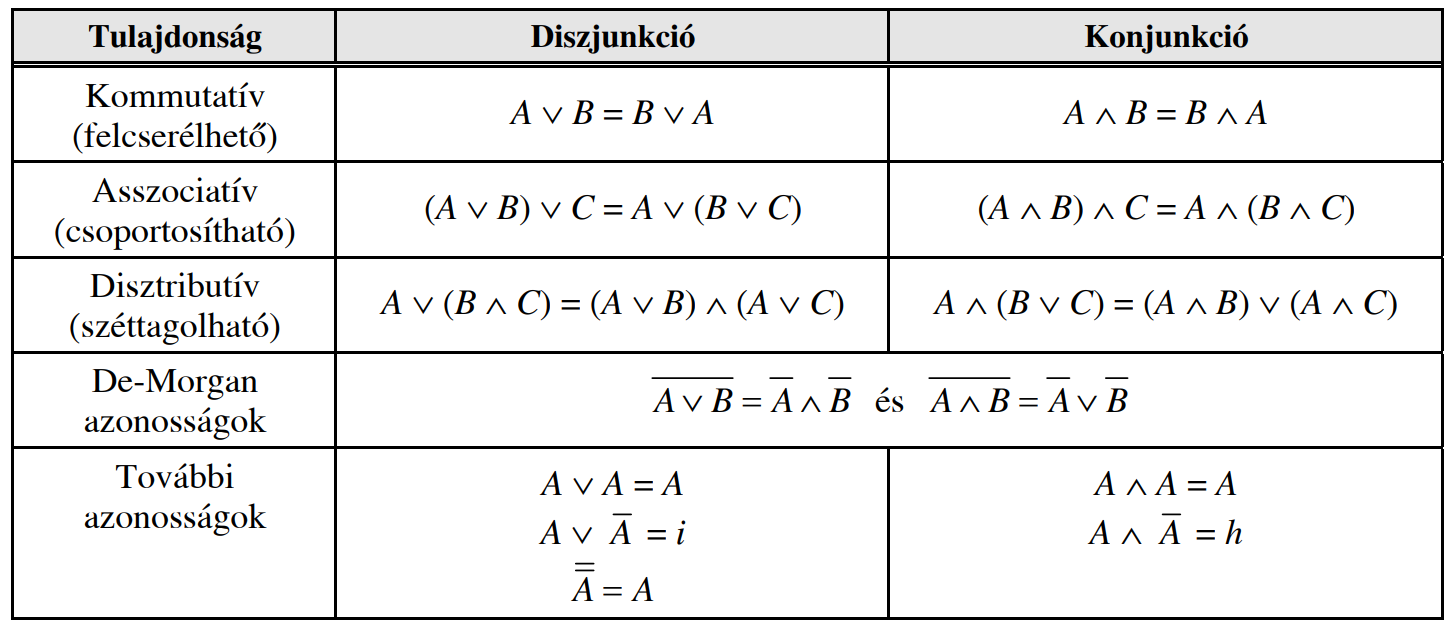
\includegraphics[width=0.8\textwidth]{logikai_muv_tul}
\end{figure}

\begin{definition}
\textbf{Állítások implikációja:} A „ha A, akkor B” kapcsolatnak megfelelő logikai műveletet implikációnak nevezzük. Az implikáció logikai értéke pontosan akkor hamis, ha A igaz és B hamis, különben az implikáció igaz. Az A állítást feltételnek, B-t következménynek nevezzük. A következtetés csak akkor hamis, ha a feltétel igaz, de a következmény hamis. Hamis állításból bármi következhet.
Jele: $A \rightarrow B$.
\end{definition}

\begin{definition}
\textbf{Állítások ekvivalenciája:} Az „A akkor és csak akkor B” kapcsolatnak megfelelő logikai műveletet ekvivalenciának nevezzük. Az ekvivalencia logikai értéke pontosan akkor igaz, ha A és B logikai értéke azonos, különben hamis. Ha az $A \leftrightarrow B$ igaz, akkor azt mondjuk, hogy A és B állítások ekvivalensek egymással.
Jele: $A \leftrightarrow B$.

Igazságtáblával:

\begin{center}
\begin{tabular}{c|c|c|c}
A & B & $A \rightarrow B$ & $A \leftrightarrow B$ \\ \hline
i & i & i & i  \\
i & h & h & h \\
h & i & i & h\\
h & h & i & i\\
\end{tabular}
\end{center}
\end{definition}

\begin{theorem}
Tetszőleges A és B kijelentésekre $A \rightarrow B = \bar{A} \lor B$
\end{theorem}

\begin{theorem}
Tetszőleges A és B kijelentésekre $A \leftrightarrow B = (A \rightarrow B) \land (B \rightarrow A)$
\end{theorem}
\begin{proof}
Igazságtáblázattal:
\begin{center}
\begin{tabular}{c|c|c|c|c|c}
$A$ & $B$ & $A \rightarrow B$ & $B \rightarrow A$ & $(A \rightarrow B) \land (B \rightarrow A)$ & $A \leftrightarrow B$ \\ \hline
$i$&$i$&$i$&$i$&$i$&$i$ \\
$i$&$h$&$h$&$i$&$h$&$h$ \\
$h$&$i$&$i$&$h$&$h$&$h$ \\
$h$&$h$&$i$&$i$&$i$&$i$ \\
\end{tabular}
\end{center}
Az ötödik oszlop igazságértékei megegyeznek az ekvivalencia igazságértékeivel, tehát az egyenlőség $A$ és $B$ minden lehetséges logikai értékére fennáll, azaz azonosság.
\end{proof}
\newpage
\subsection{Állítás és megfordítása, szükséges és elégséges feltétel}

Az állításokat gyakran „Ha $A$ igaz, akkor $B$ igaz” $(A \Rightarrow B)$ formában fogalmazzuk meg. Tehát egy $A$ állítás igazságából következik egy $B$ állítás igazsága (vagyis, ha az $A \rightarrow B$ implikáció igaz), azt mondjuk, hogy az $A$ állításból következik $B$ állítás, vagy azt, hogy $A$ állítás a $B$ állításnak \textbf{elégséges feltétele} (hiszen a $B$ állítás igazságának bizonyításához elég az $A$ állítás igazságát bizonyítani). Ilyenkor a $B$ állítás az $A$ állításnak \textbf{szükséges feltétele} (hiszen az $A$ állítás nem lehet igaz, ha a $B$ állítás nem igaz). Ha ilyen esetben az $A$ állítás igazságából a $B$ állítás igazságára következtetünk, az \textbf{helyes következtetés}.

Ha azt akarjuk kimutatni, hogy az $A$ állításból \textbf{nem} következik a $B$ állítás, elég egyetlen példát mutatni olyan esetre, amikor $A$ igaz és $B$ hamis. Ha ilyen esetben $A$ állításból a $B$ állításra következtetünk, az nem helyes, vagyis \textbf{helytelen következtetés}.

Ha az $A$ állításból következik $B$ állítás, és fordítva is: a $B$ állításból következik az $A$ állítás, akkor azt mondjuk, hogy az $A$ állításnak a $B$ állítás \textbf{szükséges és elégséges feltétele}. Jele: $A \Leftrightarrow B$ ($A$ akkor és csak akkor igaz, amikor $B$).

Ez azt jelenti, hogy $A$ és $B$ egyszerre igaz, vagyis \textbf{ekvivalensek} (egyenértékűek).

\vspace{20px}
\textbf{Példák feltételekre:}
\begin{itemize}
\item Állítás: Ha egy szám osztható 4-gyel, akkor osztható 2-vel. Ez igaz állítás.

Ekkor a 4-gyel való oszthatóság elégséges feltétele a 2-vel való oszthatóságnak, a 2-vel való oszthatóság szükséges feltétele a 4-gyel való oszthatóságnak. Vagyis a 4-gyel való oszthatóság elégséges, de nem szükséges feltétele a 2-vel való oszthatóságnak, valamint a 2-vel való oszthatóság szükséges, de nem elégséges feltétele a 4-gyel való oszthatóságnak.

\item  Állítás: Ha egy szám osztható 2-vel, akkor osztható 4-gyel. Ez hamis állítás.

Ekkor a 2-vel való oszthatóság nem elégséges feltétele a 4-gyel való oszthatóságnak, a 4-gyel való oszthatóság elégséges feltétele a 2-vel való oszthatóságnak. Vagyis a 2-vel való oszthatóság nem elégséges, de szükséges feltétele a 4-gyel való oszthatóságnak, valamint a 4-gyel való oszthatóság elégséges, de nem szükséges feltétele a 2-vel való oszthatóságnak.
\end{itemize}

Egy tétel feltételeinek és feltételei következményeinek a felcserélésével kapjuk a tétel megfordítását.

Így a fenti tétel megfordítása: „Ha $B$ igaz, akkor $A$ igaz.” $(B \Rightarrow A)$

Ha a tétel és a megfordítása is igaz, akkor a két tétel ekvivalens. $(A \Leftrightarrow B)$

Erre példa a Thalész-tétel, illetve a Pitagorasz-tétel:

\begin{theorem}[\textbf{Thalész-tétel}]
ha egy kör átmérőjének két végpontját összekötjük a kör bármely más pontjával, akkor derékszögű háromszöget kapunk.
\end{theorem}

\begin{theorem}[\textbf{Thalész-tétel megfordítása}]
ha egy háromszög derékszögű, akkor köré írható körének középpontja az átfogó felezőpontja.
\end{theorem}

\begin{theorem}[\textbf{Thalész-tétel és megfordítása összefoglalva}]
a sík azon pontjainak halmaza, amelyekből egy megadott szakasz derékszögben látszik, a szakaszhoz, mint átmérőhöz tartozó kör, elhagyva belőle a szakasz végpontjait.
\end{theorem}

\begin{theorem}[\textbf{Pitagorasz-tétel}]
ha egy háromszög derékszögű, akkor a befogók négyzetének összege egyenlő az átfogó négyzetével.
\end{theorem}

\begin{theorem}[\textbf{Pitagorasz-tétel megfordítása}]
ha egy háromszög két oldalhosszának négyzetének összege egyenlő a harmadik oldal négyzetével, akkor a háromszög derékszögű.
\end{theorem}

\subsection{Alkalmazások}
\begin{itemize}
\item Matematikai definíciók, tételek pontos kimondása, tételek bizonyítása
\item Tétel megfordításának kimondása
\item Bizonyítási módszerek kidolgozása (direkt, indirekt, skatulyaelv, teljes indukció)
\item Kombinatorika, valószínűségszámítás használja a logikai műveleteket és azok tulajdonságait
\item Automaták tervezése problémák részekre bontásával
\item A logikai műveletek és halmazműveletek párhuzamba állíthatók
\item Egyenletek, egyenlőtlenségek megoldása során sokszor végzünk logikai műveleteket (ekvivalens átalakítások).
\end{itemize}

\newpage





\section{Hatványozás, hatványfogalom kiterjesztése, a hatványozás azonosságai. Az n-edik gyök fogalma. A négyzetgyök azonosságai. Hatványfüggvények és a négyzetgyökfüggvény}

\subsection{Pozitív egész kitevőjű hatványok}
A hatványozást ugyanaz az igény hívta létre, mint a szorzást. A szorzás az ismételt összeadást jelenti, a hatványozást azonos számok szorzására vezették be, később kiterjesztették az értelmezését.

\begin{definition}[Hatványozás]
$a^n$ egy olyan ``n'' tényezős szorzat, amelynek minden tagja ``a''. \\
$$a^n = \underbrace{a\cdot a\cdot \cdots a}_{\text{n. db}} \hspace{30px} a \in \mathbb{R} \hspace{20px} n \in \mathbb{N} \setminus \lbrace0; 1\rbrace$$
\end{definition}
\begin{definition}
$$a^1=a\hspace{30px} a \in \mathbb{R}$$
\end{definition}

A hatványozás azonosságai ($a,b\in \mathbb{R}; m,n\in \mathbb{N}^+$):
\begin{enumerate}[label=\Roman*.]
\item Azonos alapú hatványokat úgy is szorozhatunk, hogy a közös alapot a kitevők összegére emeljük:
$$a^n \cdot a^m = a^{n+m}$$
\item Azonos alapú hatványokat úgy is oszthatunk, hogy a közös alapot a kitevők különbségére emeljük:
$$\dfrac{a^n}{a^m} = a^{n-m} \hspace{30px} a \neq 0 \hspace{20px} \hspace{20px} n > m$$
\item Hatványt úgy is hatványozhatunk, hogy az alapot a kitevők szorzatára emeljük:
$$\left(a^n\right)^m = a^{nm}$$
\item Szorzatot tényezőként is hatványozhatunk:
$$a^n \cdot b^n = (a\cdot b)^n$$
\item  Törtet úgy is hatványozhatunk, hogy a számlálót és a nevezőt külön-külön hatványozzuk és a kapott hatványoknak a kívánt sorrendben a hányadosát vesszük:
$$\dfrac{a^n}{b^n} = \left( \dfrac{a}{b} \right)^n \hspace{30px} b \neq 0$$
\end{enumerate}
\begin{theorem}
Azonos alapú hatványok szorzásánál a kitevő összeadódik. \\
$$a^n \cdot a^m = a^{n+m}, \hspace{30px} a \in \mathbb{R} \hspace{20px} n,m\in \mathbb{N}^+$$
\end{theorem}
\begin{proof}
\[a^n \cdot a^m = \underbrace{(a\cdot a\cdots \cdot a)}_{\text{\normalfont n db}} \underbrace{(a\cdot a\cdots \cdot a)}_{\text{\normalfont m db}}
\underbrace{=}_{\text{\normalfont a szorzás asszociatív}} \underbrace{a\cdot a\cdots \cdot a}_{\text{n+m db}} \underbrace{=}_{\text{\normalfont hatványozás definíciója}} a ^ {n+m}\]
\end{proof}

\subsection{Permanenciaelv}
A hatványozás fogalmát kiterjesztjük minden egész kitevőre, majd egész kitevőről racionális kitevőre, majd racionálisról irracionális kitevőre úgy, hogy az előbbi, pozitív egész kitevőre teljesülő azonosságok továbbra is teljesüljenek. A fogalom értelmezésének kiterjesztése esetén ezt az igényt nevezzük \textbf{permanenciaelv}nek.

\subsection{A hatványozás kiterjesztése}
A hatványozás kiterjesztése \textbf{egész kitevőkre}:
\begin{definition}
Minden szám 0. hatványa 1. \\
$$a^0 = 1 \hspace{30px} a \in \mathbb{R}\setminus \lbrace 0\rbrace$$
A $0^0$-ont nem értelmezzük, mivel ellentmondásra vezet. 
\end{definition}

\begin{definition}
Negatív egész hatványkitevő esetén az eredmény a megfelelő pozitív kitevőjű hatvány reciproka lesz. \\
$$a^{-n} = \dfrac{1}{a^n} \hspace{30px} a \in \mathbb{R}\setminus \lbrace 0\rbrace \hspace{20px} n \in \mathbb{N}^+ $$
\end{definition}


Bizonyítható, hogy ezekkel az értelmezésekkel a hatványozás azonosságai érvényben maradnak.
Pl.: a II. azonosság igaz lesz minden $n,m\in \mathbb{Z}$-re.

\vspace{50px}
A hatványozás kiterjesztése \textbf{racionális kitevőkre}:
\begin{definition}
Az ``a'' pozitív valós szám $\dfrac{p}{q}$-adik hatványa az a pozitív valós szám, amelynek ``q''-adik hatványa ``$a^p$'':
$$\left(a^{\frac{p}{q}}\right)^q=a^p, \hspace{30px}a>0\hspace{20px} p,q\in \mathbb{Z} \hspace{20px}q\neq 0$$
\end{definition}

\vspace{50px}
A hatványozás kiterjesztése \textbf{irracionális kitevőkre}:
Bármely irracionális szám tetszőlegesen közelíthető két oldalról racionális számokkal, pl.: $2^{\sqrt{2}}$, akkor a $\sqrt{2}$ értékét közelítjük nála nagyobb és kisebb racionális számokkal:
\[ 2^1 < 2^{\sqrt{2}} < 2^2  \]
\[2^{1,4} < 2^{\sqrt{2}} < 2^{1,5}\]
\[2^{1,41} < 2^{\sqrt{2}} < 2^{1,42}\]
\[2^{1,414} < 2^{\sqrt{2}} < 2^{1,415}\]
$$\vdots$$
Pontos definíció a határérték fogalmának bevezetésével adható, de bizonyítható, hogy $2^{\sqrt{2}}$ értéke létezik, és ily módon tetszőlegesen közelíthető.

Így kiterjesztettük a hatványozást minden valós kitevőre.

\subsection{Az $n$-edik gyök fogalma}

A gyökvonás művelete a hatványkitevő és a hatvány ismeretében az alap kiszámolását teszi lehetővé. Különbséget kell tenni páros és páratlan gyökkitevő között.

Az $a$ szám $n$-edik gyökének jelölése: $\sqrt[n]{a}, n \in \mathbb{N}^+,a>0$

\begin{definition}
Egy nemnegatív ``$a$'' szám négyzetgyöke az a nemnegatív szám, amelynek négyzete ``$a$''
$$\left(\sqrt{a}\right)^2=a,\hspace{30px}a\geq 0\hspace{20px} a \in \mathbb{R}$$
\end{definition}

\begin{definition}[Páros kitevőjű gyök $(2k)$ ]
Egy nemnegatív ``$a$'' szám ``$2k$''. gyöke az a nemnegatív szám, amelynek a ``$2k$''. hatványa ``$a$''
$$\left(\sqrt[2k]{a}\right)^{2k}=a,\hspace{30px}a\geq 0 \hspace{20px} k\in \mathbb{N}^+$$
\end{definition}

\begin{definition}[Páratlan kitevőjű gyök $(2k+1)$ ]
Egy valós ``$a$'' szám $(2k+1)$. gyöke az a valós szám, amelynek a $(2k+1)$. hatványa ``$a$''
$$\left(\sqrt[2k+1]{a}\right)^{2k+1}=a,\hspace{30px}a\in \mathbb{R} \hspace{20px} k\in \mathbb{N}^+$$
\end{definition}

A páros és páratlan gyökkitevőre vonatkozó definíciók közötti különbségből adódóan:
$$\left(\sqrt[2k]{a^{2k}}\right)=|a| \text{, és } \left(\sqrt[2k+1]{a^{2k+1}}\right)=a$$
$$\left(\sqrt[6]{-5^{6}}\right)=5 \text{, de } \left(\sqrt[5]{-5^{5}}\right)=-5$$


\subsection{Négyzetgyökvonás azonosságai}

\begin{enumerate}[label=\Roman*.]
\item Szorzat négyzetgyöke egyenlő a tényezők négyzetgyökének szorzatával:
$$\sqrt{a}\cdot \sqrt{b} = \sqrt{a\cdot b}, \hspace{30px} a,b\geq 0$$
\item Tört négyzetgyöke egyenlő a számláló és a nevező négyzetgyökének hányadosával:
$$\dfrac{\sqrt{a}}{\sqrt{b}} = \sqrt{\dfrac{a}{b}}, \hspace{30px} a\geq0 \hspace{20px} b>0$$
\item A hatványozás és a gyökvonás sorrendje felcserélhető egymással pozitív alap esetén:
$$\sqrt{a^k}=\left(\sqrt{a}\right)^k, \hspace{30px} a>0 \hspace{20px} k\in \mathbb{Z}$$
Figyelni kell arra, hogy a négyzetre emelés és a négyzetgyökvonás sorrendje nem cserélhető fel, ha az alap negatív. Így általánosan:
$$\sqrt{a^2}=|a|$$
\end{enumerate}

\newpage
\subsection{Hatványfüggvények és azok tulajdonságai}
\begin{definition}
Az $f:\mathbb{R}\rightarrow\mathbb{R}, f(x)=x^n$ függvényt, ahol $n\in \mathbb{N}^+$, hatványfüggvénynek nevezzük.
\end{definition}
A hatványfüggvény vizsgálatát két részre kell bontanunk aszerint, hogy ``n'' páros-e vagy páratlan:
\begin{table}[h!]
\centering
\begin{tabular}{ | m{3cm} || m{6cm} | m{6cm} | }
A függvény & $f:\mathbb{R}\rightarrow\mathbb{R}, f(x)=x^2$ & $g:\mathbb{R}\rightarrow\mathbb{R}, g(x)=x^3$ \\
\hline
Ábrázolása: &\centering 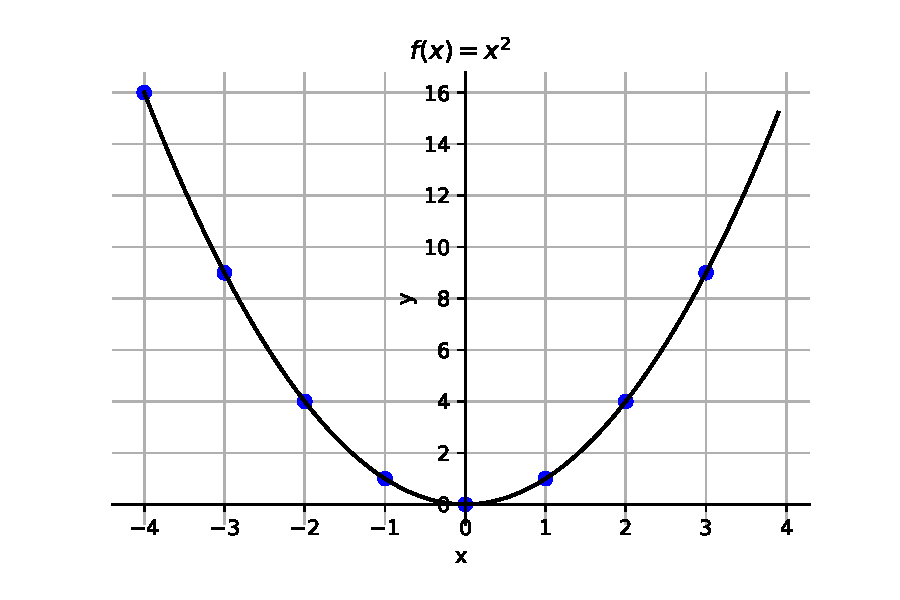
\includegraphics[width=0.4\textwidth]{chart/2021-10-31--10:23:29} & 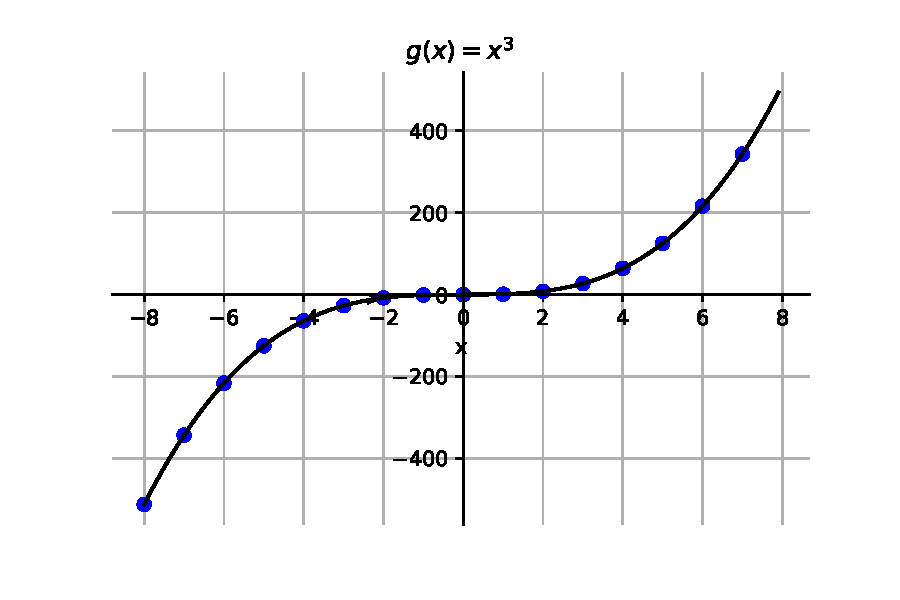
\includegraphics[width=0.4\textwidth]{chart/2021-10-31--10:27:55}\\
\hline
Értelmezési tartomány: & $D_f=\mathbb{R}$ & $D_g=\mathbb{R}$ \\
\hline
Értékkészlet: & $R_f=\mathbb{R}_0^+$ & $R_g=\mathbb{R}$\\
\hline
Zérushely: & $x = 0$& $x = 0$\\
\hline
Monotonitás: &Ha $x<0$: szig. mon. csökk, ha $x>0$: szig. mon. nő&szigorúan monoton nő \\
\hline
Szélsőérték: & globális minimum, helye: $x=0$, értéke: $y=0$ & nincs\\
\hline
Görbölüte: & konvex & ha $x < 0$: konkáv, ha $x > 0$: konvex\\
\hline
Paritás: & páros & páratlan \\
\hline
Korlátosság: & alulról korlátos, $k=0$ & nem korlátos \\
\end{tabular}
\caption{Hatványfüggvények és azok tulajdonságai}
\label{table:hatv_fugg}
\end{table}

Görbület szempontjából külön kell venni az n = 1 esetet: ekkor a függvény se nem konvex, se nem konkáv.

\newpage
\subsection{Négyzetgyökfüggvény és tulajdonságai}
\begin{definition}
Az $f:\mathbb{R}_0^+\rightarrow\mathbb{R}, f(x)=\sqrt{x}$ függvényt négyzetgyökfüggvénynek nevezzük.
\end{definition}


\begin{table}[h!]
\centering
\begin{tabular}{ | m{5cm} || c | }
A függvény & $f:\mathbb{R}_0^+\rightarrow\mathbb{R}, f(x)=\sqrt{x}$  \\
\hline
Ábrázolása: & 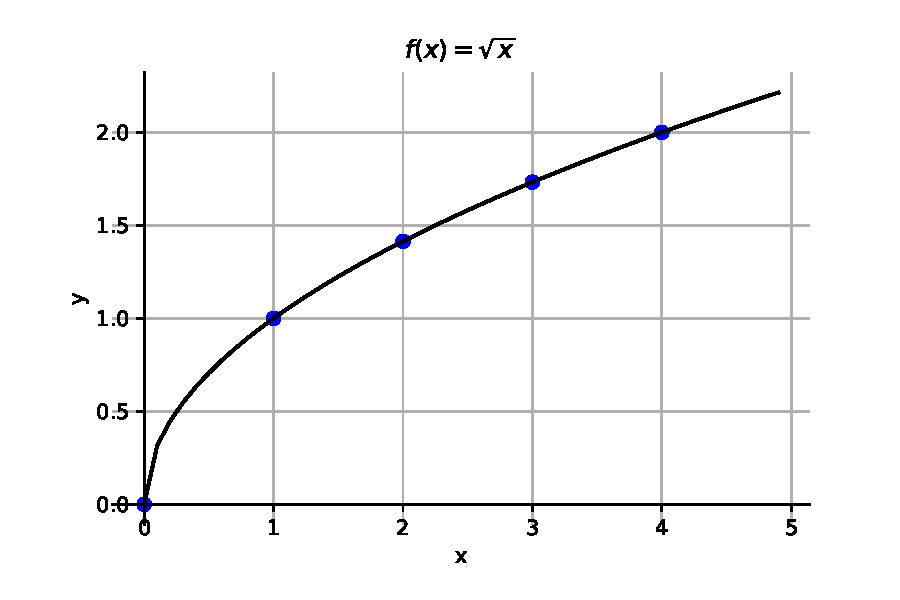
\includegraphics[width=0.4\textwidth]{chart/2021-10-31--11:04:09}\\
\hline
Értelmezési tartomány: & $D_f=\mathbb{R}_0^+$ \\
\hline
Értékkészlet: & $R_f=\mathbb{R}_0^+$ \\
\hline
Zérushely: & $x=0$\\
\hline
Monotonitás: & szigorúan monoton nő\\
\hline
Szélső érték: & globális minimum, helye: $x=0$, értéke $y=0$\\
\hline
Görbölete: & konkáv \\
\hline
Paritás: & nem páros és nem páratlan \\
\hline
Korlátosság: & alulról korlátos, $k=0$
\end{tabular}
\caption{Négyzetgyökfüggvény és tulajdonságai}
\label{table:gyok_fugg}
\end{table}

\subsection{Alkalmazások}
Hatványozás:
\begin{itemize}
\item Prímtényezős felbontásban pozitív egész kitevőjű hatványok, törtek egyszerűsítése, közös nevező keresése
\item Normálalakban: egyszerűbb a kicsi és a nagy számokkal való műveletek elvégzése
\item A számrendszerek felépítése a hatványozáson alapul
\item Mértani sorozat: $a_n$, $S_n$ kiszámolása
\item Ismétléses variációk száma: $n^k$
\item Hasonló testek felszínének aránya $\lambda^2$, térfogatának aránya $\lambda^3$
\item Kamatos kamat számítása
\item Négyzetes úttörvény: $s=\dfrac{a}{2}\cdot t^2$
\item Nevezetes azonosságok
\end{itemize}
Gyökvonás:
\begin{itemize}
\item Magasabb fokú egyenletek megoldása
\item Pitagorasz-tétel (négyzetre emelés, gyökvonás)
\item Mértani közép (gyökvonás), átlag empirikus szórása
\item Magasság-, illetve befogótétel
\item $l$ hosszúságú fonalinga lengésideje: $T=2\pi\sqrt{\dfrac{l}{g}}$
\item Harmonikus rezgőmozgás körfrekvenciája
\end{itemize}




\section{A logaritmus fogalma és azonosságai. Az exponenciális és a logaritmusfüggvény. Az inverzfüggvény}
$$2^3=8 \hspace{30px} \sqrt[3]{8}=2 \hspace{30px} \log_2 8 =3$$
\subsection{A logaritmus definíciója}

\begin{definition}
A ``b'' szám ``a'' alapú logaritmusa az a kitevő, amelyre ``a''-t emelve ``b''-t kapom.

Jele: $\log_a b$

Elnevezések: ``a'': a logaritmus alapja, ``b'': a hatványérték
$$a^{\log_ab}=b, \hspace{30px} a,b>0, \hspace{20px} a \neq 1$$

10-es alapú logaritmus:
$$\log_{10}x\rightarrow\lg x $$

Természetes alapú logaritmus:
$$\log_{e}x\rightarrow\ln x $$
$$e=2,27$$
\end{definition}

\subsection{Logaritmus azonosságai}

\begin{enumerate}[label=\Roman*.]
\item Szorzat logaritmusa egyenlő a tényezők logaritmusának összegével:
$$\log_a(x\cdot y)=\log_a x + \log_ay, \hspace{30px} x,y,a>0;\hspace{20px} a\neq 1$$
\item Tört logaritmusa megegyezik a számláló és a nevező logaritmusának különbségével:
$$\log_a\left(\dfrac{x}{y}\right)=\log_ax-\log_ay, \hspace{30px} x,y,a>0;\hspace{20px} a\neq 1$$
\item Hatvány logaritmusa az alap logaritmusának és a kitevőnek a szorzata:
$$\log_ax^k=k\cdot \log_ax, \hspace{30px} x,a>0;\hspace{20px} a\neq 1;\hspace{20px} k\in \mathbb{R}$$
\item Áttérés más alapú logaritmusra:
$$\log_ab=\dfrac{\log_cb}{\log_ca}, \hspace{30px} a,b,c>0;\hspace{20px} a,c\neq 1$$
\begin{proof}
A logaritmus definíciója alapján: $b=a^{\log_ab}$ és $a=c^{\log_ca}$

A kettő együtt: $b=\left(c^{\log_ca}\right)^{\log_ab}\underbrace{=}_{\text{III. hat. azonosság}} c^{\log_ca\cdot \log_ab}$

A logaritmus definíciója alapján: $b=c^{\log_cb}$
$$c^{\log_ca\cdot \log_ab} = c^{\log_cb}$$

Mivel az $f(x)=c^x$ fv. szigorúan monoton:
$$\log_ca\cdot \log_ab = \log_cb$$
\end{proof}
\end{enumerate}

\subsection{Exponenciális függvény}
\begin{definition}
Az $f:\mathbb{R}\rightarrow\mathbb{R}, f(x)=a^x, (a>0)$  függvényt exponenciális függvénynek nevezzük.

Az $a=1$ esetén az exponenciális függvény konstans: $f(x)=1^x=1$.
\end{definition}

\begin{table}[h!]
\centering
\begin{tabular}{ | m{3cm} || m{6cm} | m{6cm} | }
A függvény &\centering $f:\mathbb{R}\rightarrow\mathbb{R}, f(x)=a^x$, \newline ($0<a<1)$ & $g:\mathbb{R}\rightarrow\mathbb{R}, g(x)=a^x$, \newline $(1<a)$ \\
\hline
Ábrázolása: &\centering 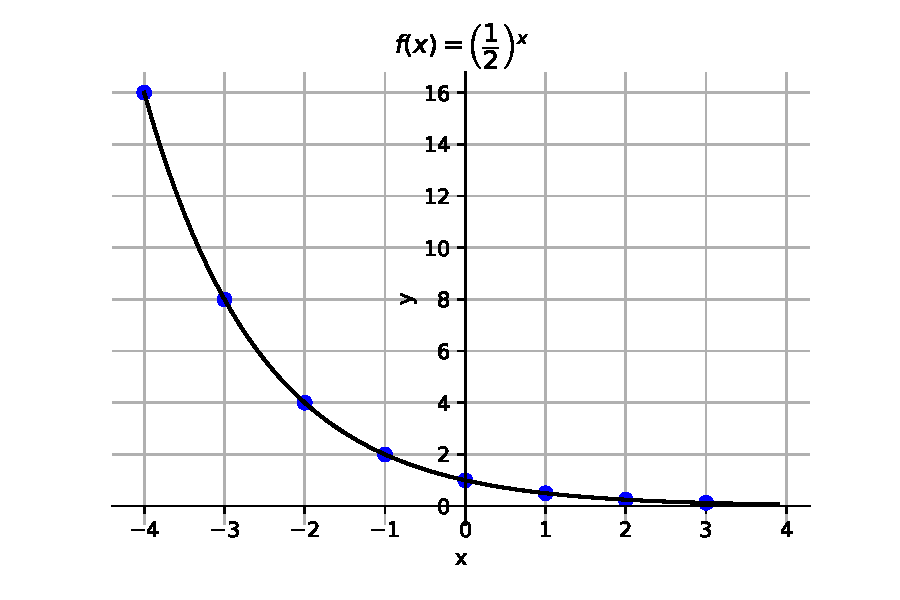
\includegraphics[width=0.4\textwidth]{chart/2021-10-31--11:54:47} & 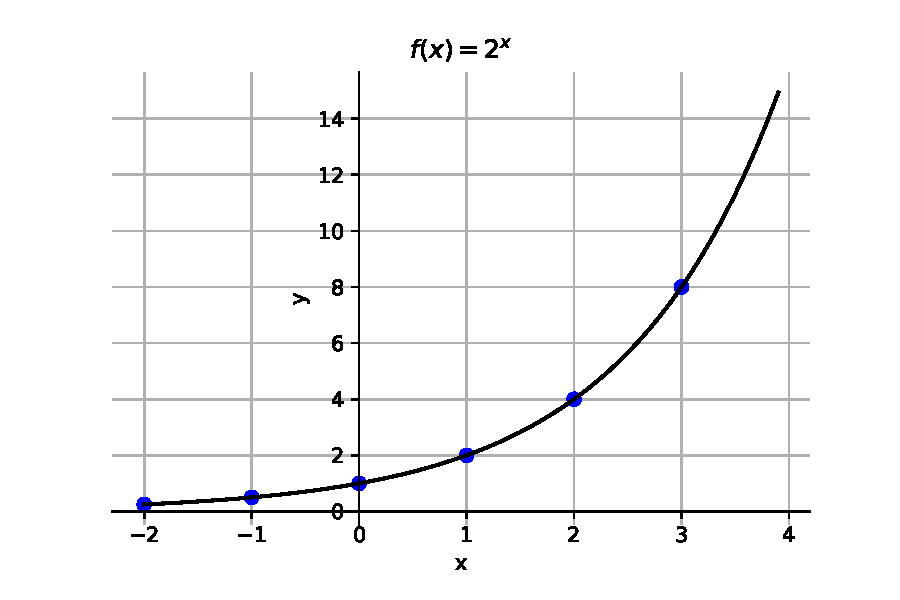
\includegraphics[width=0.4\textwidth]{chart/2021-10-31--11:55:41}\\
\hline
Értelmezési tartomány: & $D_f=\mathbb{R}$ & $D_g=\mathbb{R}$ \\
\hline
Értékkészlet: & $R_f=\mathbb{R}^+$ & $R_g=\mathbb{R}^+$\\
\hline
Zérushely: & nincs & nincs\\
\hline
Monotonitás: &szigorúan monoton csökken&szigorúan monoton nő \\
\hline
Szélsőérték: & nincs & nincs\\
\hline
Görbölüte: & konvex & konvex\\
\hline
Paritás: & nem páros és nem páratlan & nem páros és nem páratlan \\
\hline
Korlátosság: & alulról korlátos, $k=0$ & alulról korlátos, $k=0$ \\
\end{tabular}
\caption{Exponenciális függvény és tulajdonságai}
\label{table:exp_fugg}
\end{table}
\newpage
\subsection{Logaritmusfüggvény}
\begin{definition}
Az $f:\mathbb{R}^+\rightarrow\mathbb{R}, f(x)=\log_ax, (a>0, a\neq 1)$  függvényt logaritmusfüggvénynek nevezzük.
\end{definition}

\begin{table}[h!]
\centering
\begin{tabular}{ | m{3cm} || m{6cm} | m{6cm} | }
A függvény & $f:\mathbb{R}^+\rightarrow\mathbb{R}, f(x)=\log_ax$,\newline $(0<a<1)$ & $g:\mathbb{R}^+\rightarrow\mathbb{R}, g(x)=\log_ax$,\newline $(1<a)$ \\
\hline
Ábrázolása: &\centering 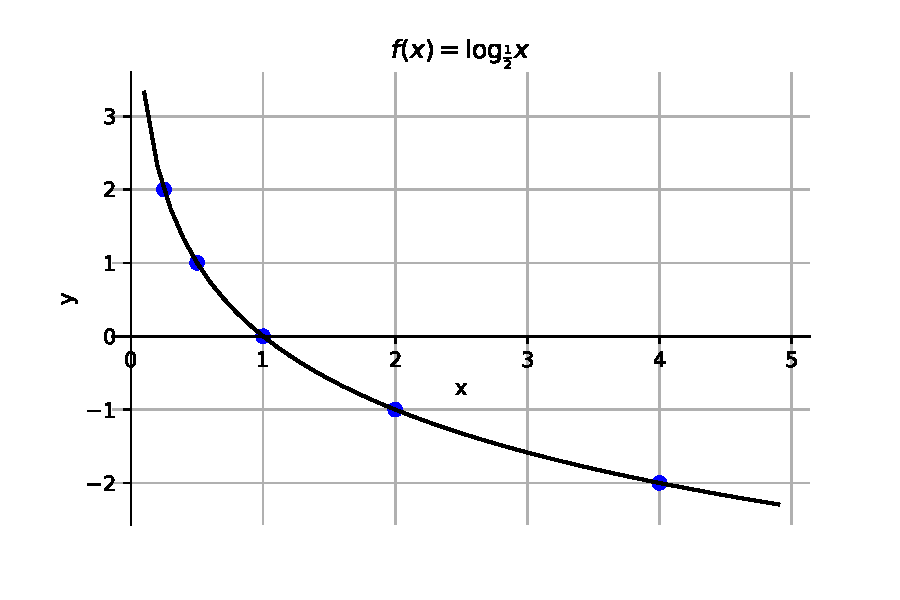
\includegraphics[width=0.4\textwidth]{chart/2021-10-31--12:59:11} & 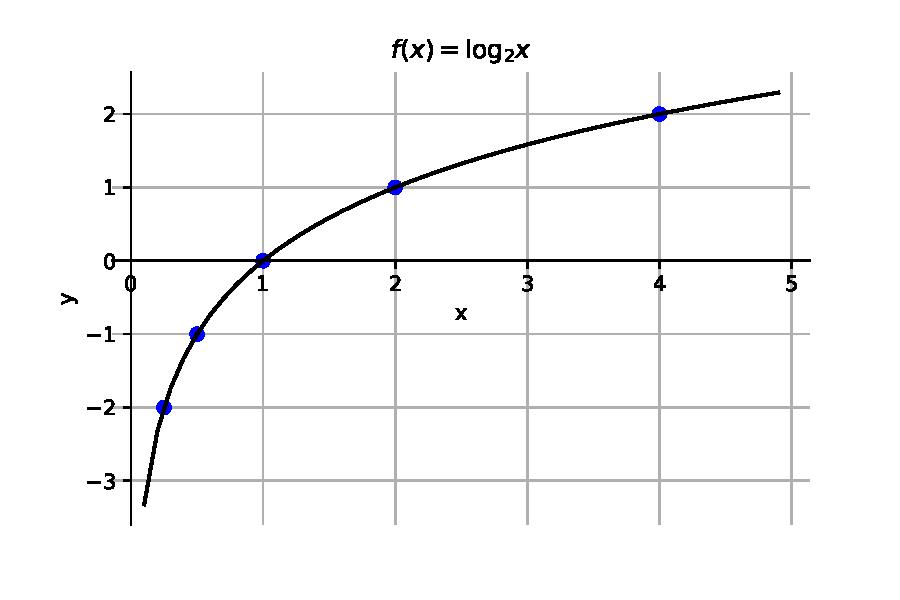
\includegraphics[width=0.4\textwidth]{chart/2021-10-31--13:00:36}\\
\hline
Értelmezési tartomány: & $D_f=\mathbb{R}^+$ & $D_g=\mathbb{R}^+$ \\
\hline
Értékkészlet: & $R_f=\mathbb{R}$ & $R_g=\mathbb{R}$\\
\hline
Zérushely: & $x = 1$& $x = 1$\\
\hline
Monotonitás: &szigorúan monoton csökken&szigorúan monoton nő \\
\hline
Szélsőérték: & nincs & nincs\\
\hline
Görbölüte: & konvex & konkáv\\
\hline
Paritás: & nem páros és nem páratlan & nem páros és nem páratlan \\
\hline
Korlátosság: & nem korlátos & nem korlátos \\
\end{tabular}
\caption{Logaritmusfüggvények és tulajdonságai}
\label{table:log_fugg}
\end{table}
Az exponenciális függvény $a\neq 1$ esetén invertálható, inverze az $f^{-1}:\mathbb{R}^+\rightarrow \mathbb{R}, f^{-1}(x)=\log_ax; a>0, a\neq 1$ logaritmusfüggvény.

A logaritmusfüggvény invertálható, inverze az $f^{-1}:\mathbb{R}\rightarrow \mathbb{R}, f^{-1}(x)=a^x; a>0, a\neq 1$ exponenciális függvény.

\subsection{Inverzfüggvény}
\begin{definition}
Az ``f'' függvény inverze a ``g'' függvény, ha az ``f'' értelmezési tartományának minden ``x'' elemére igaz, hogy f(x) eleme a ``g'' értelmezési tartományának és g(f(x)) = x. Az inverz függvény jelölése: $g=f^{-1}$

Ha az ``f'' és a ``g'' függvények egymásnak inverzei, akkor az ``f'' értelmezési tartománya a ``g'' értékkészlete, az ``f'' értékkészlete a ``g'' értelmezési tartománya.

Ha két függvény egymásnak inverzei, akkor grafikonjaik egymásnak tükörképei az $y = x$ egyenletű egyenesre.
\end{definition}

A definícióból következik, hogy csak a kölcsönösen egyértelmű függvényeknek van inverze, azaz egy függvény pontosan akkor invertálható, ha az értékkészlet minden eleme az értelmezési tartomány pontosan egy eleméhez van hozzárendelve.

Például: $f:\mathbb{R}\rightarrow\mathbb{R}^+, f(x)=2^x$ függvény és a $g:\mathbb{R}^+\rightarrow\mathbb{R}, g(x)=\log_2x$ függvény egymás inverzei, ugyanis $g(f(x))=\log_22^x=x$, illeteve $f(g(x))=2^{\log_2x}=x$, valamint az egyik függvény értelmezési tartománya a másik függvény értékkészlete és viszont.

A nem kölcsönösen egyértelmű függvényeknek nincs inverze. Ezek a függvények gyakran az értelmezési tartomány szűkítésével invertálhatóvá tehetők.

Például: a másodfokú függvény értelmezési tartományának szűkítésével invertálható, ha $f:\mathbb{R}_0^+\rightarrow\mathbb{R}^+_0, f(x)=x^2$, akkor inverze a $g:\mathbb{R}^+_0\rightarrow\mathbb{R}^+_0, g(x)=\sqrt{x}$

\vspace{30px}
\textbf{Inverz függvény előállítása:}

Egy kölcsönösen egyértelmű függvény inverze algebrai úton előállítható a változók felcserélésével
a következő módon:
\begin{enumerate}
\item $f(x)=2x-3$ függvény inverzének előállítása: $y=2x-3$ kifejezésben a változókat felcseréljük: $x=2y-3$, majd ebből az egyenletből az $y$ változót kifejezzük: $y=\dfrac{x+3}{2}$, ebből $f^{-1}(x)=\dfrac{x+3}{2}$, ahol mindkét függvény értelmezési tartománya és értékkészlete a valós számok halmaza.
\item $f(x)=\sqrt{x-2}-4$ függvény (ahol $x \geq 2$, $y \geq -4$) inverzének előállítása:

$y=\sqrt{x-2}-4$ kifejezésben a változókat felcseréljük: $x=\sqrt{y-2}-4$, majd ebből az egyenletből az $y$ változót kifejezzük: $y=(x+4)^2+2$, ebből $f^{-1}(x)=(x+4)^2+2$, (ahol $x \geq -4$, $y \geq 2$)
\end{enumerate}

\subsection{Alkalmazások}
\begin{itemize}
\item $2^x=3$ egyenlet megoldása logaritmussal: $x=\log_23$
\item Számolás számológépbe nem férő nagy számokkal, pl.: $x=\dfrac{85^{200}}{130^{120}} \Rightarrow \lg x= 200\cdot \lg 85 - 120\cdot \lg 130$
\item Gravitációs erőtérben a barometrikus magasságformulában a levegő sűrűsége a magassággal exponenciálisan csökken
\item  Exponenciális függvény írja le: a radioaktív izotópok bomlását, az oldódás folyamatát, a kondenzátor feltöltődésének és kisülésének folyamatát.
\end{itemize}
\newpage



\section{Másodfokú egyenletek és egyenlőtlenségek. Másodfokúra visszavezethető egyenletek. Egyenletek ekvivalenciája, gyökvesztés, hamis gyök, ellenőrzés}

\subsection{Egyenlet}

\begin{definition}
Az \textbf{egyenlet} bármely két egyenlőségjellel összekötött kifejezés. A kifejezésben szereplő változók az \textbf{ismeretlenek}.

Az egyenlet olyan változótól függő állítás (nyitott mondat), amelynek az alaphalmaza számhalmaz.
\end{definition}

\begin{definition}
Az \textbf{alaphalmaz} az ismeretlenek azon értékeinek halmaza, ahol az egyenletet vizsgáljuk, ahol a megoldásokat keressük.
\end{definition}

\begin{definition}
Az egyenlet \textbf{értelmezési tartománya} az alaphalmaznak az a legbővebb részhalmaza, ahol az egyenletben szereplő kifejezések értelmezhetőek.
\end{definition}

\begin{definition}
Az egyenletet igazzá tevő értékek az \textbf{egyenlet megoldásai} vagy \textbf{gyökei}.
\end{definition}

\begin{definition}
Az alaphalmaz azon elemeinek halmaza, amelyekre az egyenlet igaz, vagyis az egyenlet megoldásainak (vagy gyökeinek) halmaza az \textbf{egyenlet megoldáshalmaza} (vagy igazsághalmaza).
\end{definition}

\begin{definition}
Az \textbf{azonosság} olyan egyenlet, amelynek a megoldáshalmaza megegyezik az egyenlet értelmezési tartományával.
\end{definition}

\subsection{Másodfokú egyismeretlenes egyenlet}
\begin{definition}
\textbf{Másodfokú egyismeretlenes egyenlet} $ax^2 + bx + c = 0$ alakra hozható, ahol $a, b, c \in \mathbb{R}, a \neq 0$.

Megoldása lehetséges a megoldóképlettel, szorzattá alakítással, teljes négyzetté alakítással, Viète-formulával.
\end{definition}

\begin{theorem}
Az $ax^2 + bx + c = 0$ $(a \neq 0)$ egyenlet \textbf{megoldóképlete}: $x_{1,2}=\dfrac{-b\pm \sqrt{b^2-4ac}}{2a}$, ahol $b^2-4ac \geq 0$.
\end{theorem}
\begin{proof}
\begin{align*}
ax^2+bx+c&=0 \hspace{20px}/\cdot 4a \text{ (mivel }a\neq 0 \text{)} \\
4a^2x^2+4abx+4ac&=0
\end{align*}
teljes négyzetté alakítással:
\begin{align*}
(2ax+b)^2-b^2+4ac&=0 \\
(2ax+b)^2&=b^2-4ac
\end{align*}
Mivel a bal oldalon négyzetszám van, ami nem lehet negatív, így $b^2 - 4ac$ sem lehet az. (Ha $b^2 - 4ac<0$, akkor nincs megoldás). Ha $b^2 - 4ac \geq 0$, akkor vonjunk mindkét oldalból gyököt, figyelve, hogy elkerüljük a gyökvesztést:
\begin{align*}
|2ax+b|&=\sqrt{b^2-4ac} \\
2ax+b&=\pm \sqrt{b^2-4ac} \\
2ax&=-b\pm \sqrt{b^2-4ac} \\
x_{1,2}&=\dfrac{-b\pm \sqrt{b^2-4ac}}{2a}
\end{align*}
\end{proof}

\begin{definition}
Az $ax^2 + bx + c = 0$ $(a \neq 0)$ másodfokú egyenlet diszkriminánsa $D = b^2 - 4ac$.
\end{definition}
\begin{itemize}
\item Ha $D > 0$, akkor az egyenletnek két különböző valós gyöke van: $x_{1,2}=\dfrac{-b\pm \sqrt{b^2-4ac}}{2a}$
\item  Ha $D = 0$, akkor az egyenletnek két egymással egyenlő gyöke, vagyis 1 valódi gyöke van: $x=\dfrac{-b}{2a}$, ezt kétszeres gyöknek is nevezzük, mert $x_1 = x_2$.
\item  Ha $D < 0$, akkor az egyenletnek nincs valós gyöke.
\end{itemize}

\begin{theorem}
A másodfokú egyenlet \textbf{gyöktényezős alakja}:

Ha egy $ax^2 + bx + c = 0$ $(a \neq 0)$ egyenlet megoldható (azaz $D \geq 0$) és két gyöke van $x_1$ és $x_2$, akkor az $ax^2 + bx + c = a(x - x_1)(x - x_2)$ minden valós ``x''-re igaz.
\end{theorem}

\begin{theorem}
\textbf{Viète-formulák}: másodfokú egyenlet gyökei és együtthatói közti összefüggések:

Az $ax^2 + bx + c = 0$ $(a \neq 0)$ alakban felírt ($D \geq 0$) másodfokú egyenlet gyökeire:
$$x_1+x_2=-\dfrac{b}{a}$$
$$x_1\cdot x_2=\dfrac{c}{a}$$
\end{theorem}

\textbf{Grafikus megoldás:}

Az $x\mapsto ax^2 + bx + c = 0$ $(a\neq 0)$ függvény zérushelyei adják a megoldást. (Sőt $a > 0$ esetre törekszem!)
$$x\mapsto ax^2 + bx + c =a\left(x^2+\dfrac{b}{a}x \right)+c=a\left[\left(x+\dfrac{b}{2a} \right)^2 - \dfrac{b^2}{4a^2} \right]+c=a\left(x+\dfrac{b}{2a} \right)^2+\dfrac{4ac-b^2}{4a}$$
Olyan parabola a kép, amelynek tengelypontja $T\left(-\dfrac{b}{2a}, \dfrac{4ac-b^2}{4a} \right)$

\subsection{Másodfokú egyenlőtlenségek megoldása}

\begin{definition}
\textbf{Egyenlőtlenség}ről beszélünk, ha algebrai kifejezéseket a $<, >, \geq, \leq$ jelek valamelyikével kapcsoljuk össze. Ha ezek a kifejezések másodfokúak, akkor \textbf{másodfokú egyenlőtlenség}ről beszélünk. A másodfokú egyenlet megoldásához hasonlóan 0-ra rendezünk úgy, hogy a főegyüttható pozitív legyen, tehát a > 0. Ekkor 
ax$^2$ + bx + c < 0,
ax$^2$ + bx + c > 0,
ax$^2$ + bx + c $\leq$ 0,
ax$^2$ + bx + c $\geq$ 0 alakúra rendezhető minden másodfokú egyenlőtlenség.
\end{definition}

Az egyenlőtlenségek megoldási módszerei hasonlóak az egyenletek megoldási módszereihez:
\begin{enumerate}
\item A \textbf{mérlegelv}, alkalmazása nehézkes másodfokú egyenlőtlenségek esetében.
\item \textbf{Grafikus megoldás}: A másodfokú egyenlőtlenségek megoldásánál fontos szerepet játszik, hogy az egyenlőtlenségekben szereplő másodfokú kifejezések grafikonja a koordináta-rendszerben az $y$ tengellyel párhuzamos tengelyű parabola. Az egyenlőtlenségben szereplő másodfokú kifejezés zérushelyének megállapítása után vázlatosan ábrázoljuk a kifejezést leíró másodfokú függvényt. Majd a zérushelyek számának függvényében meghatározzuk a megoldáshalmazt. 
\end{enumerate}
\newpage
\subsection{Új ismeretlen bevezetésével másodfokúra visszavezethető egyenletek}
Magasabb fokú, illetve bizonyos exponenciális, logaritmikus, abszolút értékes, gyökös, trigonometrikus egyenletek új ismeretlen bevezetésével másodfokú egyenletre vezethetők vissza.
\[
\begin{cases}
x^6-3x^3-4=0 \\
2^{2x}-3\cdot 2^x-4=0 \\
\lg^2x-3\lg x-4=0 \\
(x-2)^2-3|x-2|-4=0 \\
x+1-3\sqrt{x+1}-4=0 \\
\sin^2 x-3\sin x-4=0
\end{cases}
\]

Ezek az egyenletek mind az $a^2 - 3a - 4 = 0$ másodfokú egyenletre vezethetők vissza új ismeretlen bevezetésével: ahol az új ismeretlen rendre 
$$a=x^3, a=2^x, a=\lg x, a=|x-2|, a=\sqrt{x+1}, a=\sin x$$

Az $a$-ra nézve másodfokú egyenlet megoldásai: $a_1 = 4, a_2 = -1$. Visszahelyettesítve az eredeti ismeretlent rendre a következőket kapjuk:
$$x^3=4 \Rightarrow x = \sqrt[3]{4}; x^3=-1 \Rightarrow x=-1$$
$$2^x=4 \Rightarrow x = 2; 2^x=-1 \Rightarrow \text{Nincs megoldás}$$
$$\lg x = 4 \Rightarrow x = 10000; \lg x = -1 \Rightarrow x = 0,1$$
$$|x-2|=4 \Rightarrow x-2=\pm 4 \Rightarrow x_1=6, x_2=-2; |x-2|=-1 \Rightarrow \text{Nincs megoldás}$$
$$\sqrt{x+1}=4 \Rightarrow x = 15; \sqrt{x+1} = -1 \Rightarrow \text{Nincs megoldás}$$
$$\sin x = 4\Rightarrow \text{Nincs megoldás}; \sin x=-1 \Rightarrow x = \dfrac{3\pi}{2}+2k\pi (k\in \mathbb{Z})$$

\subsection{Egyenletek ekvivalenciája (egyenértékűsége)}

\begin{definition}
Két egyenlet \textbf{ekvivalens}, ha alaphalmazuk és megoldáshalmazuk is azonos.
\end{definition}

\begin{definition}
\textbf{Ekvivalens átalakítás} az olyan átalakítás, amit egyenletek megoldása közben végzünk és ezzel az átalakítással az eredetivel ekvivalens egyenletet kapunk.
\end{definition}

Ekvivalens átalakítás például az egyenlet mérlegelvvel történő megoldása. Nem ekvivalens átalakítás például változót tartalmazó kifejezéssel osztani az egyenlet mindkét oldalát, vagy négyzetre emelni az egyenlet mindkét oldalát.

Az egyenletek megoldása során nem mindig van lehetőségünk ekvivalens átalakításokat végezni. Ha lehet, ilyen esetekben vagy az értelmezési tartomány, vagy az értékkészlet vizsgálatával próbálunk feltételeket felállítani.

De még így is előfordulhat, hogy olyan átalakítást végzünk, amely során
\begin{itemize}
\item az új egyenletnek szűkebb az értelmezési tartománya, mint az eredetinek, ekkor gyökvesztés állhat fenn
\item az új egyenletnek bővebb az értelmezési tartománya, mint az eredetinek, ekkor gyöknyerés állhat fenn.
\end{itemize}

\subsection{Gyökvesztés}
Gyökvesztés következhet be, ha a változót tartalmazó kifejezéssel osztjuk az egyenlet mindkét oldalát, vagy olyan átalakítást végzünk, amely szűkíti az értelmezési tartományt.

Pl. Hibás megoldás:
\begin{align*}
x^3+2x^2+x&=0 \\
x^2+2x+1&=0 \\
x&= -1
\end{align*}
Helyes megoldás:
\begin{align*}
x^3+2x^2+x&=0 \\
x(x^2+2x+1)&=0 \\
x_1&= 0 \text{ vagy } x^2+2x+1=0 \Rightarrow x_2=-1
\end{align*}

Pl. Hibás megoldás:
\begin{align*}
\lg(x+2)^2&=2\lg 5 \leftarrow D_f=\mathbb{R}\setminus \{-2\} \\
2\lg(x+2)&=2\lg 5 \leftarrow D_f= ]-2;\infty [\\
\lg(x+2)&=\lg 5 \\
x+2&=5 \\
x&=3
\end{align*}
Helyes megoldás:
\begin{align*}
\lg(x+2)^2&=2\lg 5 \leftarrow D_f=\mathbb{R}\setminus \{-2\} \\
\lg(x+2)^2&=\lg 25\\
(x+2)^2&= 25\\
x_1&=3, x_2\text{=}-7
\end{align*}

\subsection{Hamis gyök}
Hamis gyököt kaphatunk, ha az egyenlet mindkét oldalát négyzetre emeljük, vagy mindkét oldalt az ismeretlent tartalmazó kifejezéssel szorozzuk, vagy olyan átalakítást végzünk, ami bővíti az értelmezési tartományt.

\begin{enumerate}
\item $$\sqrt{7-x}=1-x \hspace{20px} \text{ Eredeti feltétel: } D_f = ]-\infty; 7] $$
A gyöknyerés kiküszöbölhető közbülső feltétellel: $1-x \geq 0 \Rightarrow D_{f_{\text{új}}}=]-\infty; 1]$
$$7-x=(1-x)^2 \Rightarrow x^2-x-6=0 \Rightarrow x_1=3 \notin D_{f_{\text{új}}}; x_2=-2 $$
\item $$2x+\dfrac{1}{x-1}=2+\dfrac{1}{x-1}$$
$$2x=2 \Rightarrow x=1$$
A gyöknyerés ekkor is kiküszöbölhető, ha az eredeti egyenletre írunk $D_f$-et.
\item $$\sqrt{x+6}-\sqrt{x+2}=\sqrt{2x+8}$$
Eredeti feltétel: $D_f=[-1; \infty[$

Ha az egyenletet először rendezzük úgy, hogy mindkét oldal nemnegatív legyen, négyzetre emeljük mindkét oldalt, rendezzük úgy, hogy a gyökös kifejezés az egyik oldalra kerüljön, a többi tag a másik oldalra, majd a négyzetre emelés előtt közbülső feltételt írunk, hogy a gyöknyerést kiküszöböljük:
$$\sqrt{x+6}=\sqrt{x+2}+\sqrt{2x+8}$$
$$x+6=x+2+2\cdot \sqrt{x+2}\cdot\sqrt{2x+8} + 2x+8$$
$$-2x-4=2\cdot \sqrt{x+2}\cdot\sqrt{2x+8}$$
közbülső feltétel írása: a jobb oldal nemnegatív, a bal oldalnak is annak kell lennie, mivel egyenlők, azaz $-2x-4\geq 0 \Rightarrow x \leq -2 \Rightarrow D_{f_{\text{új}}} = \{-2\}$ 

Ebben az esetben nem is kell elvégezni a négyzetre emelést, hiszen csak egy szám felel meg az értelmezésnek, ha van megoldás, akkor csak ez az egy szám lehet. Ennek ellenőrzésével eldönthető, hogy ez valóban megoldás-e.
\end{enumerate}

Akár a gyökvesztés, akár a hamis gyök elkerülhető, ha az egyenlet megoldása során mindig figyelünk az értelmezési tartomány változására, ha lehet, az értékkészletet is vizsgáljuk, mert így szűkíteni lehet az alaphalmazt.

\subsection{Ellenőrzés}
Egyenletek megoldásánál két szempontból is fontos szerepe van az ellenőrzésnek: ki tudjuk szűrni a megoldás során esetleg elkövetett hibáinkat, illetve ki tudjuk zárni a hamis gyököket. Ez utóbbiak elkerülhetők, ha a megoldás során nem bővítjük az értelmezési tartományt.

A kapott megoldásokat behelyettesítéssel ellenőrizni kell, így el lehet dönteni, hogy az eredeti egyenletnek is megoldásai-e, vagy csak az átalakítottnak.

\subsection{Alkalmazások}
\begin{itemize}
\item Egyenes, kör, parabola adott abszcisszájú vagy ordinátájú pontjának meghatározása
\item Magasabb fokú egyenletek megoldása
\item Pitagorasz-tétel
\item Koszinusztételből oldal kiszámítása
\item Mély szakadék mélységének meghatározása: egy ledobott kő dobásától a szakadék alján történő koppanás hangjának meghallásáig eltelt idő mérésével
\end{itemize}

\newpage


\section{A leíró statisztika jellemzői, diagramok. Nevezetes középértékek}
\subsection{Adatsokaságok jellemzői}

\begin{definition}
A statisztika feladatai közé tartozik, hogy bizonyos egyedek meghatározott tulajdonságairól tájékozódjék, majd a szerzett (általában számszerű) adatokat feldolgozza, elemzi. Az elemzéshez összegyűjtött adatok halmazát adatsokaságnak, mintának, a meghatározott tulajdonságot ismérvnek, változónak nevezzük. A sokaság elemeinek az ismérv szerinti tulajdonságát statisztikai adatnak, az adatsokaság elemeinek számát a sokaság méretének nevezzük.
\end{definition}

\subsection{A leíró statisztika jellemzői}
A leíró statisztika a tömegesen előforduló jelenségekkel, a jelenségekből nyert adatok vizsgálatával, elemzésével (leírásával) foglalkozik.

A statisztika egyik fontos feladata az adatok összegyűjtése. Ha a vizsgálandó egyedek száma nagyon nagy, akkor nem minden egyedet vizsgálunk meg a tulajdonság alapján, hanem az adatsokaságnak vesszük egy részhalmazát, vagyis az egyedek közül \textbf{mintát veszünk}. A megfelelően kiválasztott minta elemzéséből következtethetünk a sokaság adataira.

A \textbf{reprezentatív mintavétel}nél törekedni kell arra, hogy a vizsgált tulajdonság előfordulása a mintában közelítse a sokaságban való előfordulását. Pl. közvélemény-kutatás.

\textbf{Véletlenszerű mintavétel}nél a sokaság elemei egyenlő valószínűséggel kerülnek a mintába. Pl. urnából húzás.

\begin{definition}
Az egyes adatok előfordulásának a száma a \textbf{gyakoriság}. Az adatok összehasonlíthatósága miatt sokszor a gyakoriságnak a teljes adatsokasághoz viszonyított arányával, a \textbf{relatív gyakorisággal} dolgozunk, azaz a gyakoriságot osztjuk az adatok számával.
\end{definition}

\textbf{Osztályokba} soroljuk az adatokat, ha nagy méretű (sok adatból álló) adatsokasággal dolgozunk, vagy ha sok különböző érték van közel azonos gyakorisággal a sokaságban, akkor az egymáshoz közeli értékek összevonásával az adatokat osztályokba rendezzük. Az osztályba sorolásnál fontos szempont, hogy az osztályoknak diszjunktaknak (különállóknak), de hézagmentesnek kell lennie.

\subsection{Diagramok}
Az adatok grafikus megjelenítése diagramon történik, amelynek típusát a feladat határozza meg.

\textbf{Oszlopdiagram}: az adatok egymáshoz való viszonyát ábrázolja. Nem célszerű használni, ha az adatok közt van 1-2 kiugró érték (túl nagy: nem fér rá a diagramra, túl kicsi: eltörpül a többi oszlop közt), vagy ha az adatok közötti eltérés nagyon kicsi (közel azonosnak látszanak az értékek). A vízszintes tengelyen az adatfajtáknak megfelelő intervallumokat jelöljük, ezek fölé olyan téglalapokat rajzolunk, amelyeknek területe arányos az adatfajta gyakoriságával.

\textbf{Hisztogram (gyakorisági diagram)}: az adatok gyakorisági eloszlását oszlopdiagramon ábrázolja úgy, hogy az oszlopok hézagmentesen helyezkednek el.

\textbf{Sávdiagram}: fordított oszlopdiagram, amelyben a két tengely helyet cserél, az oszlopok vízszintesek, azaz sávok.

\textbf{Kördiagram}: a részadatoknak az egészhez való viszonyát ábrázolja. Alkalmas \%-os formában megadott adatok ábrázolására. A teljes szög (360$^\circ$) 100\%-nak felel meg, a megfelelő százalékérték egyenesen arányos a körcikk középponti szögével. Nem célszerű használni, ha nagyon sok az adat (túl kicsik a középponti szögek, nem összehasonlíthatók)

\textbf{Vonaldiagram}: koordináta-rendszerben pontként ábrázolja az összetartozó számpárokat, és ezeket töröttvonallal köti össze. Különböző adatok (pl. időbeli) változását ábrázolja. A gyakoriságok vonaldiagramját gyakorisági poligonnak nevezzük.

\subsection{Statisztikai mutatók}
\textbf{A középértékek}

Az adatsokaság egészét csak leegyszerűsítéseket alkalmazva tudjuk jellemezni. Ezt a célt szolgálják a \textbf{középértékek}, amelyek egyetlen számmal írnak le egy adathalmazt.

Ezek előnye, hogy megfelelően alkalmazva jól jelenítik meg az egész adatsokaság valamilyen tulajdonságát, ugyanakkor hátrányuk, hogy nem nyújtanak képet az egyes adatokról.

\begin{definition}
Egy adatsokaságban a leggyakrabban előforduló adat a minta \textbf{módusz}a.

Ha a legnagyobb gyakoriság csak egyszer fordul elő az adatsokaságban, akkor az egymóduszú, ha többször is előfordul, akkor többmóduszú, tehát a módusz több elem is lehet, ha ugyanakkora a gyakoriságuk.

A módusz előnye, hogy könnyen meghatározható, hátránya, hogy csak akkor ad használható
jellemzést a mintáról, ha a többi adathoz képest sokszor fordul elő.
\end{definition}

\begin{definition}
Az adatok összegének és az adatok számának hányadosa \textbf{a minta átlaga (számtani közepe)}.

Ha egyes adatok többször is előfordulnak, akkor az összegben szorozni kell őket a gyakoriságukkal és az összeget a gyakoriságok összegével osztjuk. Ez a \textbf{súlyozott számtani közép}.

Az átlag fontos tulajdonsága, hogy a nála nagyobb adatoktól vett eltéréseinek összege
egyenlő a nála kisebb adatoktól vett eltéréseinek összegével.

Hátránya, hogy egyetlen, a többitől jelentősen eltérő adat eltorzíthatja, így ekkor már nem jól
jellemzi a mintát.
\end{definition}

\begin{definition}
Páratlan számú adat \textbf{medián}ja a nagyság szerinti sorrendjükben a középső adat, páros számú adat mediánja pedig a két középső adat átlaga.

A definícióból adódik, hogy az összes előforduló ismérvérték (adat) fele kisebb vagy egyenlő, fele nagyobb vagy egyenlő, mint a medián.

Fontos tulajdonsága, hogy az adatoktól mért távolságainak összege minimális.
A medián előnye, hogy valóban középérték, hiszen ugyanannyi adat nagyobb nála, mint ahány kisebb.
\end{definition}

\textbf{A szóródás jellemzői}


\begin{definition}
Az adatok legnagyobb és legkisebb elemének a különbségét a \textbf{minta terjedelmé}nek nevezzük.

Minél kisebb a minta terjedelme, annál jobban jellemzi a mintát.
\end{definition}

\begin{definition}
 Az adatok átlagtól való eltérések négyzetének átlaga a \textbf{minta szórásnégyzete}, ennek négyzetgyöke a \textbf{minta szórása}: \[S=\sqrt{\dfrac{\sum\limits_{i=1}^n(x_i-\bar{x})^2}{n}}\]

A szórás megmutatja, hogy a minta adatai mennyire térnek el az átlagtól. Minél kisebb a szórás, annál jobban jellemzi az átlag az adatsokaságot.
\end{definition}

\subsection{Pozitív számok nevezetes középértékei}

\begin{definition}
$a_1, a_2, a_3, ..., a_n$ pozitív számok
\begin{itemize}
\item számtani (aritmetikai) közepe: $$A=\dfrac{a_1+a_2+a_3+...+a_n}{n}$$
\item mértani (geometriai) közepe: $$G=\sqrt[n]{a_1\cdot a_2\cdot a_3\cdot ...\cdot a_n}$$
\item négyzetes (kvadratikus) közepe: $$Q=\sqrt{\dfrac{a_1^2+a_2^2+a_3^2+...+a_n^2}{n}}$$
\item harmonikus közepe: $$H=\dfrac{n}{\dfrac{1}{a_1}+\dfrac{1}{a_2}+\dfrac{1}{a_3}+...+\dfrac{1}{a_n}} \text{\normalfont , ha }a_1, a_2, a_3, ..., a_n>0$$
\end{itemize}
\end{definition}

\begin{theorem}
Középértékek közti összefüggés: $H\leq G\leq A \leq Q$.
 
Egyenlőség akkor és csak akkor, ha $a_1=a_2=a_3=...=a_n$.
\end{theorem}

\begin{theorem}
Két pozitív valós szám esetén $\sqrt{a\cdot b}\leq \dfrac{a+b}{2}$
\end{theorem}
\begin{proof}
Mivel az egyenlőtlenség mindkét oldala pozitív, ezért a négyzetre emelés az eredetivel ekvivalens állítást fogalmaz meg. Tehát
$$ab\leq \dfrac{a^2+2ab+b^2}{4}\text{  /}\cdot \text{4}$$
$$4ab\leq a^2+2ab+b^2\text{  /-4}ab$$
$$0\leq a^2-2ab+b^2 \text{ /nevezetes szorzattá alakítjuk}$$
$$0\leq (a-b)^2$$

Az utolsó egyenlőtlenség igaz, így az eredeti is az.

Az eredmény alapján megállapítható, hogy a két közép akkor és csak akkor lesz egymással egyenlő, ha $a = b$. Ekkor $a=\sqrt{ab}=\dfrac{a+b}{2}=b$.
\end{proof}

\subsection{Nevezetes középértékek alkalmazása szélsőérték-feladatokban}
\textbf{1. Összeg állandósága esetén a szorzatot tudjuk maximalizálni.}

Pl.: Azon téglatestek közül, amelyek éleinek összege 60 cm, melyiknek a térfogata maximális?

Legyenek a téglatest élei: $a$, $b$ és $c$.

Ekkor a téglatest térfogata $V = abc$, az élek összege: $4(a + b + c) = 60$.

Ebből $a + b + c = 15$.

A számtani és mértani közép közti egyenlőtlenséget kihasználva:
$$\dfrac{a+b+c}{3}\geq \sqrt[3]{abc}\Rightarrow \left(\dfrac{a+b+c}{3} \right)^3\geq abc\Rightarrow \left(\dfrac{15}{3} \right)^3\geq abc \Rightarrow 5^3\geq abc \Rightarrow 125\geq V$$
Mivel egyenlőség csak $a = b = c$ esetén teljesül, így a térfogat az 5 cm élű kocka esetén maximális.

\vspace{20px}
\textbf{2. Szorzat állandósága esetén az összeget tudjuk minimalizálni.}

Pl.: Azon téglalapok közül, amelyeknek a területe 100 cm$^2$, melyiknek a kerülete a minimális?

Legyenek a téglalap oldalai $a$ és $b$.

Ekkor a téglalap területe $t = ab = 100$, kerülete $k = 2(a + b)$, amiből $\dfrac{k}{4}=\dfrac{a+b}{2}$.

A számtani és mértani közép közti egyenlőtlenséget kihasználva:

$$\dfrac{a+b}{2}\geq \sqrt{ab}\Rightarrow \dfrac{k}{4}\geq \sqrt{100}\Rightarrow \dfrac{k}{4}\geq 10\Rightarrow k\geq 40$$
Mivel egyenlőség csak $a = b$ esetén teljesül, így a kerület a 10 cm oldalú négyzet esetén minimális.

\vspace{20px}
Pl.: $f: \mathbb{R^+}\rightarrow \mathbb{R}, f(x)=x+\dfrac{1}{x}$. Határozzuk meg az $f(x)$ függvény minimumát!

A számtani és mértani közép közti egyenlőtlenséget kihasználva:

$$\dfrac{x+\dfrac{1}{x}}{2}\geq \sqrt{x\cdot \dfrac{1}{x}}\Leftrightarrow x+\dfrac{1}{x}\geq 2\cdot \sqrt{1}\Leftrightarrow x+\dfrac{1}{x}\geq 2 \Leftrightarrow 	f(x)\geq 2$$.

Ekkor az $f$ minimumának értéke $f(x) = 2$, minimum helye: $x=\dfrac{1}{x}=1$.

\subsection{Alkalmazások}
\begin{itemize}
\item Statisztika
\begin{itemize}
\item közvélemény-kutatások
\item szavazások
\item gazdasági mutatók
\item osztályátlagok, hiányzási statisztikák
\item felvételi átlagpontok
\end{itemize}
\item Nevezetes középértékek
\begin{itemize}
\item számtani közép: statisztikai átlag kiszámítása
\item mértani közép: átlagos növekedési ütem kiszámítása, magasságtétel, befogótétel
\item négyzetes közép: statisztikai szórás kiszámítása
\item harmonikus közép: átlagsebesség meghatározása
\end{itemize}
\end{itemize}
\newpage





\section{Függvénytani alapismeretek, függvények tulajdonságai, határérték, folytonosság. Számsorozatok. A számtani sorozat, az első $n$ tag összege}
\subsection{Függvény fogalma, értelmezési tartomány, értékkészlet}

\begin{definition}
Legyen A és B két nem üres halmaz. Azt mondjuk, hogy megadunk egy A halmazon értelmezett B-beli értéket felvevő \textbf{függvény}t, ha A minden eleméhez hozzárendeljük a B egy és csakis egy elemét. Jele: $f: A \rightarrow B$.
\end{definition}

\begin{definition}
\textbf{Értelmezési tartomány}nak nevezzük az A halmazt. Jele $D_f$.
\end{definition}

\begin{definition}
\textbf{Értékkészlet} a B halmaz azon elemeiből álló halmaz, amelyek a hozzárendelésnél fellépnek (vagyis az $f(x)$ értékek). Jele az $R_f$.
\end{definition}

\begin{definition}
Ha $c \in D_f$, akkor a c helyen felvett függvényértéket $f(c)$-vel jelöljük, ez a helyettesítési vagy \textbf{függvényérték}.
\end{definition}

\begin{definition}
Ha az értelmezési tartomány és az értékkészlet is számhalmaz, akkor a függvényt grafikonon tudjuk szemléltetni. A \textbf{grafikon} az $(x; f(x))$ pontok halmaza.
\end{definition}

\subsection{Függvénytulajdonságok}

\textbf{Lokális függvénytulajdonságok:} zérushely, monotonitás, lokális (helyi) szélsőérték, görbület,
inflexió, pontbeli folytonosság.

\begin{definition}
\textbf{zérushely:} Az értelmezési tartomány azon $x_0$ eleme, ahol a függvény értéke 0, azaz $f(x_0) = 0$.
\end{definition}

\begin{definition}
\textbf{monotonitás:} Az f függvény az értelmezési tartományának egy intervallumában monoton \textbf{nő}, ha az intervallum minden olyan $x_1, x_2$ helyén, amelyre $x_1 < x_2$, akkor $f(x_1) \leq f(x_2)$ teljesül.

Az f függvény az értelmezési tartományának egy intervallumában monoton \textbf{csökken}, ha az intervallum minden olyan $x_1, x_2$ helyén, amelyre $x_1 < x_2$, akkor $f(x_1) \geq f(x_2)$ teljesül.

Ha az egyenlőtlenségben az egyenlőség nincs megengedve, akkor \textbf{szigorú monotonitás}ról beszélünk.
\end{definition}

\begin{definition}
\textbf{lokális (helyi) szélsőérték:} Az f függvénynek az $x_0 \in D_f$ helyen \textbf{lokális maximum}a van, ha az $x_0$-nak van olyan I környezete, amelynek minden $x \in D_f$ pontjában $f(x) \leq f(x_0)$. Az $x_0$ helyet lokális (helyi) maximumhelynek nevezzük.

Az f függvénynek az $x_0 \in D_f$ helyen \textbf{lokális minimum}a van, ha az $x_0$-nak van olyan I környezete, amelynek minden $x \in D_f$ pontjában $f(x) \geq f(x_0)$. Az $x_0$ helyet lokális (helyi) minimumhelynek nevezzük.

A monotonitás és a szélsőérték definíciójából következik, hogy ahol a függvény monotonitást vált, ott lokális szélsőértéke van.
\end{definition}
\newpage
\begin{definition}
\textbf{görbület:} A függvényt egy intervallumban \textbf{konvex}nek nevezzük, ha az intervallum bármely két $x_1, x_2$ pontjára teljesül az $f\left(\dfrac{x_1+x_2}{2}\right) \leq \dfrac{f(x_1)+f(x_2)}{2} $ egyenlőtlenség.

Ha az egyenlőtlenség fordított irányú, akkor a függvény \textbf{konkáv} az adott intervallumon.

Szemléletesen a konvex (illetve konkáv) görbékre jellemző, hogy a görbe bármely két pontját összekötő szakasz a görbe felett (illetve alatt) halad.
\begin{figure}[h]
\centering
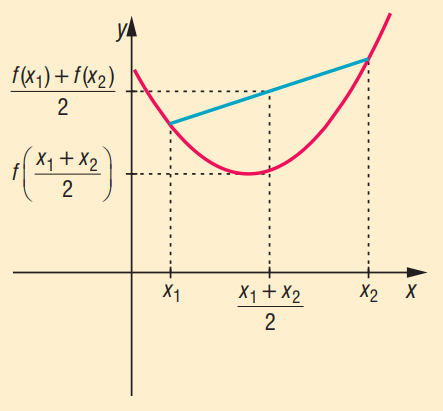
\includegraphics[width=0.3\textwidth]{konvexitas_def}
\end{figure}
\end{definition}

\begin{definition}
\textbf{inflexió:} A függvénygörbének azt a pontját, ahol a görbe konvexből konkávba, vagy konkávból konvexbe megy át, \textbf{inflexiós pont}nak nevezzük.
\end{definition}

\begin{definition}
\textbf{pontbeli folytonosság:} Az f függvény az értelmezési tartománynak egy $x_0$ pontjában \textbf{folytonos}, ha létezik az $x_0$ pontban határértéke és az megegyezik a helyettesítési értékkel, vagyis $f(x_0)=\lim\limits_{x \rightarrow x_0} f(x)$.
\end{definition}

\textbf{Globális függvénytulajdonságok:} értelmezési tartomány, értékkészlet, globális (abszolút) szélsőérték, paritás, periodikusság, intervallumbeli folytonosság, korlátosság.

\begin{definition}
\textbf{globális (abszolút) szélsőérték:} Az f függvénynek az $x_0 \in D_f$ helyen \textbf{globális maximum}a van, ha minden $x \in D_f$ pontjában $f(x) < f(x_0)$. Az $x_0$ helyet globális maximumhelynek nevezzük.

Az f függvénynek az $x_0 \in D_f$ helyen \textbf{globális minimum}a van, ha minden $x \in D_f$ pontjában $f(x) > f(x_0)$. Az $x_0$ helyet globális minimumhelynek nevezzük.

Tehát a szélsőérték abszolút (globális) szélsőérték $x_0$-ban, ha az értelmezési tartomány minden pontjára igazak az egyenlőtlenségek.
\end{definition}

\begin{definition}
\textbf{paritás:} Az f függvény \textbf{páros}, ha értelmezési tartományának minden x elemére –x is eleme az értelmezési tartománynak, továbbá az értelmezési tartomány minden x elemére $f(x) = f(-x)$.

Az f függvény \textbf{páratlan}, ha értelmezési tartományának minden x elemére –x is eleme az értelmezési tartománynak, továbbá az értelmezési tartomány minden x elemére $f(x) = -f(-x)$.

A páros függvénynek a grafikonja tengelyesen szimmetrikus az y tengelyre. (pl. $x \mapsto x^{2n}, x \mapsto |x|, x \mapsto \cos x$)

A páratlan függvények grafikonja középpontosan szimmetrikus az origóra. (pl. $x \mapsto x ^{2n + 1}, x \mapsto \dfrac{1}{x} , x \mapsto \sin x, x \mapsto \tg x$).
\end{definition}

\begin{definition}
\textbf{periodikusság:} Az f függvény \textbf{periodikus}, ha létezik olyan $p \neq 0$ valós szám, hogy a függvény értelmezési tartományának minden x elemére $x + p$ is eleme az értelmezési tartománynak, továbbá az értelmezési tartomány minden x elemére $f(x + p) = f(x)$, a legkisebb ilyen p a függvény periódusa (pl. trigonometrikus függvények, törtrész függvény).
\end{definition}

\begin{definition}
\textbf{intervallumbeli folytonosság:} Az f függvény egy nyílt intervallumban folytonos, ha az intervallum minden pontjában folytonos (pl.: folytonos: $x \mapsto x^n, x \mapsto \log_a x, x \mapsto a^x, x \mapsto \sin x, x \mapsto \cos x; \text{nem folytonos: egészrész}, x \mapsto \dfrac{1}{x} , x \mapsto \tg x, x \mapsto \ctg x$.)
\end{definition}

\begin{definition}
\textbf{korlátosság:} Az f függvény \textbf{felülről korlátos} az értelmezési tartományának egy intervallumában, ha létezik olyan K szám, hogy az intervallum minden x pontjában $f(x) \leq K$. Egy függvény felső korlátai közül a legkisebbet a függvény \textbf{felső határ}ának (szuprémumának) nevezzük.

Az f függvény \textbf{alulról korlátos} az értelmezési tartományának egy intervallumában, ha létezik olyan k szám, hogy az intervallum minden x pontjában $f(x) \geq k$. Egy függvény alsó korlátai közül a legnagyobbat a függvény \textbf{alsó határ}ának (infimumának) nevezzük.

\textbf{Korlátos} egy függvény, ha alulról és felülről is korlátos.
\end{definition}

\subsection{Számsorozat}
\begin{definition}
A \textbf{számsorozat} olyan függvény, amelynek értelmezési tartománya a pozitív egész számok halmaza, értékkészlete pedig valamilyen számhalmaz.

Az $a_1, a_2, ..., a_n$ tagokból álló sorozatot $\{a_n\}$-nel vagy $(a_n)$-nel jelöljük. A sorozat n-edik tagja: $a_n$.
\end{definition}

\textbf{Sorozatok megadása történhet:}

\begin{itemize}
\item Függvényszerűen: $f: \mathbb{N}^+ \rightarrow \mathbb{R}, x \mapsto x^2$, tagjai: 1, 4, 9, 16...
\item Az $n$-edik általános tagot előállító formulával: $a_n = 3 \cdot 2^n$
\item Az elemeit egyértelműen meghatározó utasítással: $\{a_n\} = \{2^n \text{utolsó számjegye}\}$
\item A sorozat tagjaival: 3, 6, 9, 12, 15, 18, ...
\item Rekurzív módon: megadjuk a sorozat első néhány tagját, valamint a képzési szabályt, amellyel a sorozat következő tagjai a megelőzőkből megkaphatók.

Pl.: \textit{Fibonacci sorozat:} $a_1 = 1, a_2 = 1, a_n = a_{n - 1} + a_{n - 2}$, ha $n\geq 3$. A tagok: 1, 1, 2, 3, 5, 8, 13, 21 ...
\end{itemize}

\subsection{Sorozatok tulajdonságai}

\begin{definition}
Az $\{a_n\}$ sorozat \textbf{szigorúan monoton növő}, ha minden pozitív egész n-re teljesül: $a_n < a_{n + 1}$.
\end{definition}

\begin{definition}
Az $\{a_n\}$ sorozat \textbf{szigorúan monoton csökkenő}, ha minden pozitív egész n-re teljesül: $a_n > a_{n + 1}$.
\end{definition}

Ha nem a szigorú monotonitást, csak a monotonitást kérjük, akkor megengedett az egyenlőség is.

Ha egy sorozat monotonitását keressük, akkor általában nem az $a_n \lessgtr a_{n+1}$ kapcsolatot vizsgáljuk, hanem vagy $a_{n+1}-a_n \lessgtr 0$, vagy $\dfrac{a_{n+1}}{a_n}\lessgtr 1$.


\begin{itemize}
\item Ha a sorozat szigorúan monoton növő, akkor $a_{n+1}-a_n > 0$, illetve $\dfrac{a_{n+1}}{a_n} > 1$
\item Ha a sorozat szigorúan monoton csökkenő, akkor $a_{n+1}-a_n < 0$, illetve $\dfrac{a_{n+1}}{a_n} < 1$
\end{itemize}

Ha bármelyik esetben a reláció mellett az egyenlőség is teljesül, akkor a sorozat csak monoton. Többnyire a feladat típusa dönti el, hogy melyik módszerrel vizsgáljuk a sorozat monotonitását. Magasabb kitevőjű vagy faktoriálist tartalmazó összefüggések esetén célszerű a hányadossal való vizsgálat, gyakrabban használjuk a különbséggel való számolást.

\begin{definition}
Egy $\{a_n\}$ sorozatnak K felső korlátja, ha $a_n \leq K$ minden pozitív egész n-re teljesül. Ilyenkor a sorozatot \textbf{felülről korlátos}nak nevezzük.
\end{definition}

\begin{definition}
Egy $\{a_n\}$ sorozatnak k alsó korlátja, ha $a_n \geq k$ minden pozitív egész n-re teljesül. Ilyenkor a sorozatot \textbf{alulról korlátos}nak nevezzük.
\end{definition}

\begin{definition}
 Egy sorozat \textbf{korlátos}, ha alulról és felülről is korlátos.
\end{definition}

\begin{definition}
A felülről korlátos sorozat legkisebb felső korlátját a sorozat \textbf{felső határ}ának, alulról korlátos sorozat legnagyobb alsó korlátját a sorozat \textbf{alsó határ}ának nevezzük.
\end{definition}

\begin{theorem}
 Felülről korlátos sorozatnak van felső határa, alulról korlátos sorozatnak van alsó határa.
\end{theorem}

\begin{theorem}
Végtelen sok egymásba skatulyázott, zárt intervallumnak van közös pontja. Ha az intervallumok hossza minden pozitív számnál kisebbé válik, akkor pontosan egy közös pont van.
\end{theorem}

\begin{definition}
Az $\{a_n\}$ sorozat \textbf{konvergens} és \textbf{határértéke} az A szám, ha minden pozitív $\varepsilon$ számhoz létezik olyan N pozitív egész, hogy a sorozat $a_N$ utáni tagjai mind az A szám $\varepsilon$ sugarú környezetébe esnek, vagyis minden pozitív $\varepsilon$ számhoz létezik olyan N pozitív egész, hogy minden $n > N$ esetén $|a_n - A|<\varepsilon$. Jelölése: $\lim\limits_{n \to \infty} a_n=A$, vagy $a_n \to A$.

Ez szemléletesen azt jelenti, hogy bármilyen kis pozitív $\varepsilon$-ra a sorozatnak csak véges sok tagja esik az $]A - \varepsilon, A + \varepsilon[$ intervallumon kívülre.
\end{definition}

\begin{definition}
Az olyan sorozatokat, amelyeknek nincs határértéke, \textbf{divergens} sorozatoknak nevezzük.
\end{definition}

\begin{theorem}
A konvergens sorozatok tulajdonságai:
\begin{itemize}
\item Konvergens sorozatnak csak egy határértéke van.
\item Ha egy sorozat konvergens, akkor korlátos.
\item Ha egy sorozat monoton és korlátos, akkor konvergens. A sorozat határértéke monoton növekedés esetében a sorozat felső, monoton csökkenés esetében a sorozat alsó határa.
\item Ha minden $n\in \mathbb{N}^+$-ra $a_n\leq b_n \leq c_n$ és $a_n\to A, c_n\to A$, akkor $b_n\to A$. Ez a redőelv.
\end{itemize}
\end{theorem}

\subsection{Számtani sorozat}
\begin{definition}
Azt a számsorozatot, amelyben a második tagtól kezdve bármely tag és a közvetlenül előtte álló tag különbsége állandó, \textbf{számtani sorozat}nak nevezzük. Ez a különbség a \textbf{differencia}, jele d.

Ha egy számtani sorozatnál
\begin{itemize}
\item $d > 0$, akkor a sorozat szigorúan monoton növő, és alulról korlátos.
\item $d = 0$, akkor a sorozat konstans.
\item $d < 0$, akkor a sorozat szigorúan monoton csökkenő, és felülről korlátos.
\end{itemize}
\end{definition}

\begin{theorem}
 Ha egy \textbf{számtani sorozat} első tagja $a_1$, differenciája d, akkor n-edik tagja $a_n = a_1 + (n - 1)d$.
\end{theorem}

\begin{theorem}
A \textbf{számtani sorozat első n tagjának összege} $(S_n)$ az első és az n-edik tag számtani közepének n-szeresével egyenlő: $S_n=\dfrac{a_1+a_n}{2}\cdot n$
\end{theorem}
\begin{proof}
az összeget felírjuk az 1., aztán az n-edik tagtól kiindulva:

$S_n=a_1+a_2+a_3+...+a_{n-2}+a_{n-1}+a_n$

$S_n=a_n+a_{n-1}+a_{n-2}+...+a_3+a_2+a_1$

$S_n=a_1+(a_1+d)+(a_1+2d)+...+(a_1+(n-3)d)+(a_1+(n-2)d)+(a_1+(n-1)d)$

$S_n=a_n+(a_n-d)+(a_n-2d)+...+(a_n-(n-3)d)+(a_n-(n-2)d)+(a_n-(n-1)d)$

Összeadva:
$2S_n=\underbrace{(a_1+a_n)+(a_1+a_n)+...+(a_1+a_n)}_{n}$.

$$2S_n=(a_1+a_n)\cdot n$$
$$S_n=\dfrac{a_1+a_n}{2}\cdot n$$
\end{proof}

\begin{theorem}
$S_n$ másik alakja: $S_n=\dfrac{2a_1+(n-1)d}{2}\cdot n$
\end{theorem}

\begin{theorem}
Tetszőleges elem a tőle szimmetrikusan elhelyezkedőknek a számtani közepe: $a_n=\dfrac{a_{n-k}+a_{n+k}}{2}$.
\end{theorem}

Számtani sorozat konvergenciája: Csak $d = 0$ esetén konvergens a számtani sorozat.

\subsection{Alkalmazások}
\begin{itemize}
\item A Fibonacci-sorozat elemeivel sok helyen találkozhatunk a természetben. Például a fenyőtoboz, az ananász pikkelyei, a napraforgó magjai Fibonacci-spirálban helyezkednek el.
\item  Speciális sorozatok határértéke:
\begin{itemize}
\item $\lim\limits_{n\to \infty}\dfrac{1}{n}=0$
\item $\lim\limits_{n\to \infty}\left(1+\dfrac{1}{n} \right)^n=e$, ami a természetes alapú logaritmus alapszáma (Euler típusú sorozat).
\item Következmény: $\lim\limits_{n\to \infty}\left(1+\dfrac{\alpha}{n} \right)^n=e^\alpha$
\item $\lim\limits_{n\to \infty} q^n=\begin{cases} 0, & \text{ha } |q|<1 \\ \infty, & \text{ha } q>1 \\ \text{nem létezik}, & \text{ha } q\leq -1 \\ 1, & \text{ha }q=1 \end{cases}$. Ez a mértani sorozat.
\end{itemize}
\item Analízis: függvény határértékénél, folytonosságánál
\item Irracionális kitevőjű hatvány fogalma sorozat határértékével
\end{itemize}
\newpage






\section{Mértani sorozat, az első $n$ tag összege, végtelen mértani sor. Kamatszámítás, gyűjtőjáradék, törlesztőrészlet. Exponenciális folyamatok a társadalomban és a természetben}
\subsection{Mértani sorozat, a sorozat általános tagja, az első $n$ tag összege}
\begin{definition}
A \textbf{számsorozat} olyan függvény, amelynek értelmezési tartománya a pozitív egész számok halmaza, értékkészlete pedig valamilyen számhalmaz.

Az $a_1, a_2, ..., a_n$ tagokból álló sorozatot $\{a_n\}$-nel vagy $(a_n)$-nel jelöljük. A sorozat n-edik tagja: $a_n$.
\end{definition}

\begin{definition}
Azt a számsorozatot, amelyben a második tagtól kezdve bármely tag és a közvetlenül előtte álló tag hányadosa állandó, \textbf{mértani sorozat}nak nevezzük. Ez a hányados a \textbf{kvóciens}, jele q.

A definíció kizárja, hogy a sorozat bármely eleme 0 legyen, továbbá a hányados sem lehet 0.
\end{definition}

\begin{theorem}
Ha egy \textbf{mértani sorozat} első tagja $a_1$, hányadosa q, akkor \textbf{n-edik tagja}: $a_n=a_1\cdot q^{n-1}$.
\end{theorem}
\begin{theorem}
A mértani sorozat első n tagjának összege:
\begin{itemize}
\item ha $q=1$, akkor $S_n=n\cdot a_1$
\item ha $q\neq 1$, akkor $S_n=a_1\cdot \dfrac{q^{n}-1}{q-1}$.
\end{itemize}
\end{theorem}

\begin{proof}
A két esetben:
\begin{itemize}
\item ha $q=1$, akkor a sorozat minden tagja $a_1$, így $S_n=\overbrace{a_1+a_1+...+a_1}^{n}=n\cdot a_1$
\item ha $q\neq 1$, akkor az összeget írjuk fel $a_1$-gyel, és $q$-val:
$$S_n=a_1+a_1q+a_1q^{2}+...+a_1q^{n-2}+a_1q^{n-1}$$
Szorozzuk meg mindkét oldalt $q$-val:
$$S_nq=a_1q+a_1q^2+a_1q^{3}+...+a_1q^{n-1}+a_1q^{n}$$
Vonjuk ki a két egyenletet egymásból:
$$S_nq-S_n=a_1q^{n}-a_1$$
$$S_n(q-1)=a_1(q^n-1)$$
Osszuk mindkét oldalt $(q - 1) \neq 0$-val:
$$S_n=a_1\cdot \dfrac{q^{n}-1}{q-1}$$
így állításunkat beláttuk.
\end{itemize}
\end{proof}

\begin{theorem}
Bármely elem négyzete egyenlő a tőle szimmetrikusan elhelyezkedő tagok szorzatával: $a_n^2=a_{n-k}\cdot a_{n+k}$
\end{theorem}

\begin{theorem}
Pozitív tagú sorozatnál bármely elem a tőle szimmetrikusan elhelyezkedő elemek mértani közepe: $a_n=\sqrt{a_{n-k}\cdot a_{n+k}}$
\end{theorem}

Mértani sorozat konvergenciája:
\begin{itemize}
\item $a_n\to a_1$, ha $q=1$.
\item $a_n\to 0$, ha $|q|<1$.
\item $\{a_n\}$ divergens, ha $q=-1$, vagy $|q|>1$.
\end{itemize}

\subsection{Végtelen mértani sor}

\begin{definition}
Legyen adott egy $\{a_n\}$ számsorozat. Az $a_1+a_2+a_3+...+a_{n-1}+a_n+...$

végtelen sok tagú összeget \textbf{végtelen sor}nak (vagy röviden sornak) nevezzük.

Jelölés: $a_1+a_2+a_3+...+a_{n-1}+a_n+...=\sum\limits^\infty_{i=1}a_i$.
\end{definition}

\begin{definition}
Ha az $a_1+a_2+a_3+...+a_{n-1}+a_n+...$ végtelen sorban az $a_1, a_2, a_3, ..., a_{n-1}, a_n, ...$ tagok egy mértani sorozat tagjai, akkor a sort \textbf{mértani sor}nak nevezzük.

Felmerül a kérdés, hogy mit értsünk végtelen sok szám összegén, hiszen a véges sok szám esetén megszokott módszerek nem alkalmazhatók.
\end{definition}

\begin{definition}
A \textbf{sor összegé}n az
\begin{align*}
S_1&=a_1 \\
S_2&=a_1+a_2 \\
... \\
S_n&=a_1+a_2+a_3+...+a_n \\
\end{align*}
úgynevezett részletösszegek sorozatának határértékét értjük, amennyiben ez a határérték létezik. Tehát a sor összegét egy olyan sorozat határértékével definiáljuk, amely sorozat első tagja $a_1$, n-edik tagja az eredeti sorozat első n tagjának összege.
\end{definition}
\begin{theorem}
Ha egy mértani sorban $|q|<1$, akkor a mértani sor konvergens, és összege $S=\dfrac{a_1}{1-q}$, ha $|q|\geq 1$, akkor nem konvergens.
\end{theorem}
\newpage
\subsection{Kamatszámítás}
Pénzügyi folyamatokban \textbf{kamat} a kölcsönadott, illetve a letétbe helyezett pénzösszeg, vagyis a \textbf{tőke} használatáért járó díj egy adott időszakra. A kamat nagyságát a tőke százalékában fejezzük ki, ez a kamatláb $(p\%)$. De számolhatunk kamattényezővel ($q$) is, ami a kamatláb 100-ad részével tér el az 1-től: értéknövekedés esetén $q=1+\dfrac{p}{100}$, értékcsökkenés esetén $q=1-\dfrac{p}{100}$.

\textbf{Kamatos kamat}ról akkor beszélünk, ha a kamatozási időszak végén a kamatot hozzáadják a tőkéhez, és utána ez a megnövekedett érték kamatozik.

A kamatos kamat számítása a mértani sorozat alkalmazásának olyan speciális esete, amikor a sorozatnak van nulladik tagja, amit a pénzügyi számításokban $a$-val (annuitás rövidítése) jelölünk.

\textit{Kamatoskamat-számítás:} ha egy a összeg $p\%$-kal kamatozik évente, akkor az $n$-edik év végére az
összeg $a_n=a\cdot\left(1+\dfrac{p}{100} \right)^n$. Ha $q=1+\dfrac{p}{100}$ kamattényező, akkor $a_n = a \cdot q^n$. Ez olyan mértani sorozat $n$-edik eleme, amelynek első eleme $aq$, hányadosa $q$.

Az $a_n$ összefüggésében négy mennyiség szerepel, közülük bármely hármat ismerve a negyedik kiszámolható.

A kamatozás üteme nemcsak éves, hanem havi, napi stb. is lehet. Ekkor figyelni kell arra, hogy a kamattényező és az időszak hossza azonos nagyságú időszakra vonatkozzon.

Ha az éves kamatláb $p\%$, az éves kamattényező $q$, akkor a havi kamattényező $\sqrt[12]{1+\dfrac{p}{100}}=\sqrt[12]{q}$, hasonlóan a napi kamattényező $\sqrt[365]{1+\dfrac{p}{100}}=\sqrt[365]{q}$.

\subsection{Gyűjtőjáradék}
Gyűjtőjáradékról akkor beszélünk, ha egy alapösszeget egyenlő időközönként ugyanakkora öszszeggel növelünk, vagyis egyenlő időközönként azonos összeget elhelyezünk a bankban ugyanazon a számlán, vagyis gyűjtjük a pénzt, és minden betett összegünk kamatos kamattal kamatozik.

\textit{Gyűjtőjáradék számítása:} minden év elején egy a összeget teszünk a bankba, és ez $p\%$-kal kamatozik évente úgy, hogy a következő év elején a megnövekedett összeghez tesszük hozzá az újabbat.

Ha a kamattényező $q=1+\dfrac{p}{100}$, akkor az $n$-edik év végén a rendelkezésre álló összeg egy olyan
mértani sorozat első $n$ elemének összege, ahol $a_1 = aq$. Ekkor az $n$-edik év végére $S_n=aq\cdot \dfrac{q^n-1}{q-1}$ összeget gyűjtünk.

\subsection{Törlesztőrészlet}
Törlesztőrészletről akkor beszélünk, ha egy hitelt egyenlő időközönként ugyanakkora összeggel fizetünk vissza, azaz egyenlő időközönként azonos összeggel csökkentjük a tartozásunkat, vagyis törlesztjük a hitelt, minden befizetett összeg után csak a fennálló tartozásra fizetünk kamatos kamatot.

\textit{Törlesztőrészlet számítása:} felveszünk $n$ évre $S_n$ nagyságú hitelt évi $p\%$-os kamatra, és minden évben $a$ összeget törlesztünk. Az $n$-edik év végére a befizetéseknek kamatokkal megnövelt értékének egyenlő kell lennie a kölcsön $n$ év alatt $p\%$-os kamatozással megnőtt értékével. Ha $q=1+\dfrac{p}{100}$ a kamattényező, akkor a hitelre fennálló összefüggés: $S_n\cdot q^n=a\cdot \dfrac{q^n-1}{q-1}$.



\subsection{Exponenciális folyamatok a társadalomban és a természetben}
A társadalomban és a természetben lejátszódó exponenciális folyamatok fő típusai az időben, illetve a térben lejátszódó exponenciálisan növekedő, illetve csökkenő folyamatok.

Az időben lezajló exponenciális növekedést a $N_t=N_0\cdot e^{\lambda t}$, a csökkenést a $N_t=N_0\cdot e^{-\lambda t}$képlet írja le, ahol $N_0$ a kezdeti mennyiség és $N_t$ a $t$ időpontbeli mennyiség. Az exponenciális folyamatra jellemző a $\lambda$ paraméter, amit rendszerint pozitívnak választanak csökkenés esetén is.

Az exponenciálisan növekedő mennyiségek minél nagyobbak, annál gyorsabban növekszenek.

A növekedés mértéke arányos a mennyiség nagyságával. Az exponenciálisan növekvő mennyiségek változását exponenciális függvény írja le.

Az exponenciális változás lehet folytonos (pl. populáció növekedése), illetve diszkrét (pl. kamatos
kamat).

Az egyik legjellemzőbb probléma a Föld túlnépesedése. Egy matematikai modell szerint a népesség 1837 óta (akkor a lakosság kb 1 milliárd volt) az előző évinek 1,1\%-ával növekedett. Ez azt jelenti, hogy 1837 óta a Föld lakosságát leíró képlet: $N_t=1\cdot 1,011^t$. A modell szerint Föld lakossága kb 63 évente megduplázódik $(1,011^{63} \approx 2)$. Mai ismereteink szerint a 2026-ra adott 8 milliárd lakos becslés közel áll a valósághoz. Az exponenciális népességnövekedés ezek szerint azt is jelenti, hogy ugyanannyi időközönként egyre nagyobb számmal növekszik a népesség. A rendelkezésre álló erőforrások – például energia, nyersanyag, élelem – azonban nem tudnak lépést tartani ezzel a növekedéssel. Így vagy az életfeltételek romlanak drámaian, vagy a népesség növekedési ütemének kell drasztikusan csökkennie.

A természetben a populációk növekedési folyamata kezdetben exponenciális függvénnyel írható le (ideális körülmények között: táplálékbőség, ragadozók hiánya). Előbb-utóbb azonban eljön a telítődés ideje, amikor is a növekedés különböző okok miatt erősen lelassul; a természetben ilyen okok a terület eltartóképessége és a fajtársak vetélkedése.

A diszkrét exponenciális növekedés leggyakoribb felhasználási területe a kamatos kamat számítása, ekkor a kamatot évente egyszer és nem a kamat keletkezésének időpontjában tőkésítik, vagyis veszik hozzá a tőkéhez.

A diszkrét exponenciális csökkenés elsősorban a tárgyak (pl. autó, számítógép) értékcsökkenésének számolása, ekkor a csökkenés mértéke az előző időszak százalékában adott. Évi $p\%$-os értékcsökkenés esetén $n$ év múlva a tárgy értéke: $a_n=a\cdot\left(1-\dfrac{p}{100} \right)^n$. Pl. ha évente $11\%$-kal csökken a tárgy értéke, akkor kb 6 év alatt a tárgy értéke a felére csökken, a 6 év ebben az esetben a tárgy értékének felezési ideje.

Térben exponenciális folyamat pl az egyes sugárzások elnyelődése homogén közegben. Ezek hasonló képletekkel írhatók fel, mint az időben exponenciális folyamatok, de idő helyett a távolság a változó.

Az exponenciális folyamatok lényege tehát az, hogy egyenlő időközök alatt mindig ugyanannyiszorosára változik a vizsgált mennyiség.
\newpage
\subsection{Alkalmazások}
\begin{itemize}
\item Végtelen szakaszos tizedes törtek közönséges tört alakra hozásakor a konvergens mértani sor tulajdonságait használjuk
\item $\lim\limits_{n\to \infty} q^n=\begin{cases} 0, & \text{ha } |q|<1 \\ \infty, & \text{ha } q>1 \\ \text{nem létezik}, & \text{ha } q\leq -1 \\ 1, & \text{ha }q=1 \end{cases}$. Ez a mértani sorozat.
\item Az $N=N_0\cdot e^{-\lambda (t-t_0)}$ bomlási törvényben, ahol $N$ a még el nem bontott részecskék száma, $N_0$ a kezdeti részecskeszám, $\lambda$ az anyagra jellemző bomlási állandó. A felezési idő alatt a radioaktív atomok száma a kezdeti érték felére csökken, akármelyik pillanat az idő mérésének kezdete
\item  Exponenciális függvénnyel írható le, azaz mértani sorozat szerint változó folyamatok pl a radioaktív izotópok bomlási egyenletei, vagy az oldódás folyamata, a kondenzátor feltöltődésének és kisülésének folyamata, baktériumok számának változása
\end{itemize}
\newpage





\section{A differenciálhányados fogalma, deriválási szabályok. A differenciálszámítás alkalmazásai (érintő, függvényvizsgálat, szélsőértékfeladatok)}

\subsection{Függvény fogalma, értelmezési tartomány, értékkészlet}

\begin{definition}
Legyen A és B két nem üres halmaz. Azt mondjuk, hogy megadunk egy A halmazon értelmezett B-beli értéket felvevő \textbf{függvény}t, ha A minden eleméhez hozzárendeljük a B egy és csakis egy elemét. Jele: $f: A \rightarrow B$.
\end{definition}

\begin{definition}
\textbf{Értelmezési tartomány}nak nevezzük az A halmazt. Jele $D_f$.
\end{definition}

\begin{definition}
\textbf{Értékkészlet} a B halmaz azon elemeiből álló halmaz, amelyek a hozzárendelésnél fellépnek (vagyis az $f(x)$ értékek). Jele az $R_f$.
\end{definition}

\begin{definition}
Ha $c \in D_f$, akkor a c helyen felvett függvényértéket $f(c)$-vel jelöljük, ez a helyettesítési vagy \textbf{függvényérték}.
\end{definition}

\begin{definition}
Ha az értelmezési tartomány és az értékkészlet is számhalmaz, akkor a függvényt grafikonon tudjuk szemléltetni. A \textbf{grafikon} az $(x; f(x))$ pontok halmaza.
\end{definition}

\subsection{Differenciálhányados}

\begin{definition}
Legyen f egy $]a, b[$ intervallumon értelmezett függvény és $x_0$ az értelmezési tartomány egy pontja. Ekkor a $g(x)=\dfrac{f(x)-f(x_0)}{x-x_0}$ függvényt az f függvény $x_0$ ponthoz tartozó különbségi hányados (\textbf{differenciahányados}) függvényének nevezzük.
\begin{figure}[h]
\centering
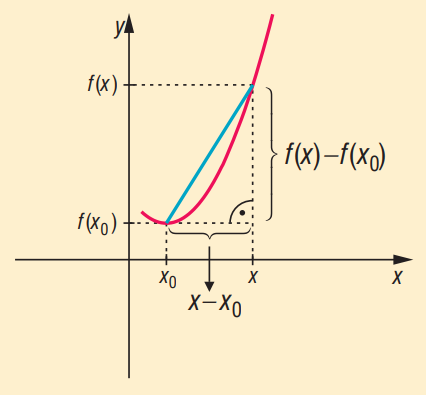
\includegraphics[width=0.3\textwidth]{differencialhanyados}
\end{figure}
\end{definition}

\begin{definition}
Az f függvény $x_0$ ponthoz tartozó különbségi hányadosának az $x_0$ helyen vett határértékét (ha ez a határérték létezik és véges) az f függvény $x_0$ pontbeli \textbf{differenciálhányados}ának vagy deriváltjának nevezzük.

Jel: $f'(x_0)=\lim\limits_{x\to x_0}\dfrac{f(x)-f(x_0)}{x-x_0}$.
\end{definition}
\newpage
\begin{definition}
Ha egy függvénynek egy pontban van deriváltja, akkor azt mondjuk, hogy a függvény ebben a pontban differenciálható (deriválható).

Az $x_0$ pontbeli differenciálhányados egy ábrázolható függvény esetében a függvény grafikonjának $(x_0, f(x_0))$ pontjához húzott érintő meredeksége.

Pl.: $f: \mathbb{R}\to \mathbb{R}, f(x)=x^2-4x+5$.

Differenciahányados $x_0 = 1$ pontban:
$$g(x)=\dfrac{(x^2-4x+5)-(1^2-4\cdot 1+5)}{x-1}=\dfrac{x^2-4x+3}{x-1}=\dfrac{(x-3)(x-1)}{x-1}=x-3\text{, ha }x\neq 1$$
g nincs értelmezve az $x = 1$ helyen, de $\lim\limits_{x\to 1}(x-3)=-2$ létezik és véges $\Rightarrow f'(x)=-2$. Tehát a parabola érintőjének meredeksége $x=1$ helyen -2.

Differenciahányados $x_0$-ban (ha $x\neq x_0$):
$$g(x)=\dfrac{(x^2-4x+5)-(x_0^2-4x_0+5)}{x-x_0}=\dfrac{x^2-x_0^2-4x+4x_0}{x-x_0}=$$
$$=\dfrac{(x+x_0)(x-x_0)-4(x-x_0)}{x-x_0}=\dfrac{(x-x_0)(x+x_0-4)}{x-x_0}=x+x_0-4$$

$f'(x_0)=\lim\limits_{x\to x_0}(x+x_0-4)=2x_0-4\Rightarrow$ tetszőleges $x$ pontban: $f'(x)=2x-4$.
\end{definition}

\begin{definition}
Ha f függvénynél az értelmezési tartomány minden olyan pontjához, ahol f differenciálható hozzárendeljük a differenciahányados értékét, akkor az f függvény \textbf{differenciálhányados (derivált) függvény}ét kapjuk. Jelölés: $f'(x)$.
\end{definition}

\subsection{Deriválási szabályok}
\begin{theorem}
Az f és g függvények deriválhatóak az x helyen, és deriváltjuk itt $f'(x)$, illetve $g'(x)$:
\begin{enumerate}
\item $f(x)=c, c =$ állandó $\Rightarrow f'(x)=0$
\item $(c\cdot f(x))'=c\cdot f'(x), c\in\mathbb{R}$
\item $(f(x)\pm g(x))'=f'(x)\pm g'(x)$
\item $(f(x)\cdot g(x))'=f'(x)\cdot g(x) + f(x)\cdot g'(x)$
\item $\left(\dfrac{f(x)}{g(x)} \right)'=\dfrac{f'(x)\cdot g(x) - f(x)\cdot g'(x)}{g^2(x)}$
\item $(f(g(x)))'=f'(g(x))\cdot g'(x)$
\end{enumerate}
\end{theorem}
\begin{theorem}
\textbf{Elemi függvények deriváltjai:}
\begin{enumerate}
\item $(x^n)'=n\cdot x^{n-1}$, ha $x>0, n\in\mathbb{N}^+$.
\item $(a^x)'=a^x\cdot \ln a$, ha $a>0, a\neq 1$.

$(e^x)'=e^x$.
\item $(\log_a x)'=\dfrac{1}{x\cdot \ln a}$, ha $a>0, a\neq 1, x>0$.
\item $(\ln x)'=\dfrac{1}{x}$, ha $x>0$.
\item $(\sin x)'=\cos x$
\item $(\cos x)'=-\sin x$
\end{enumerate}
\end{theorem}
\newpage
\begin{theorem}
Hatványfüggvény deriváltfüggvénye: $(x^n)'=n\cdot x^{n-1}$, ha $x>0, n\in\mathbb{N}^+$.
\end{theorem}
\begin{proof}
teljes indukcióval
$n=1$-re igaz: $f(x)=x^1$ esetében
\begin{itemize}
\item [bal oldal:] $f'(x_0)=\lim\limits_{x\to x_0}\dfrac{f(x)-f(x_0)}{x-x_0}=\lim\limits_{x\to x_0}\dfrac{x-x_0}{x-x_0}=\lim\limits_{x\to x_0}1=1\Rightarrow (x^1)'=1$
\item [jobb oldal:] $1\cdot x^{1-1}=1\cdot x^0=1\cdot 1$
\end{itemize}
$\Rightarrow$ Igaz

Tegyük fel, hogy $n = k$-ra igaz: $(x^k)'=k\cdot x^{k-1}$.

Bizonyítjuk az öröklődést: $(x^{k+1})'=(k+1)\cdot x^k$.

Bal oldal:
$$(x^{k+1})'\underbrace{=}_{\text{hatv. azon.}}(x\cdot x^k)'\underbrace{=}_{\text{szorzat deriváltja}}x'\cdot x^k+x\cdot (x^k)'=1\cdot x^k+x\cdot k \cdot x^{k-1}=x^k+k\cdot x^k=(k+1)\cdot x^k$$
Ez pedig pontosan a jobb oldal, ezzel állításunkat bebizonyítottuk.
\end{proof}

\subsection{A differenciálszámítás alkalmazásai}

\textbf{Függvény adott pontbeli érintője:}

Ha az $f(x)$ függvény az $x_0$ pontban differenciálható, akkor grafikonjának az $(x_0; f(x_0))$ pontban van érintője és $f'(x_0)$ ebben a pontban az érintő meredeksége. Ekkor a függvény $x_0$-beli érintőjének egyenlete: $y = f'(x_0) \cdot (x - x_0) + f(x_0)$.

\vspace{20px}
\textbf{Függvényvizsgálat:}

\begin{theorem}
Az f függvény az $]a, b[$ intervallum minden pontjában differenciálható. Ha az intervallum minden x pontjában
\begin{itemize}
\item $f'(x)>0$, akkor f az $]a, b[$-n \textbf{szigorúan monoton nő}
\item $f'(x)<0$, akkor f az $]a, b[$-n \textbf{szigorúan monoton csökken}
\item $f'(x)\geq 0$, akkor f az $]a, b[$-n \textbf{monoton nő}
\item $f'(x)\leq 0$, akkor f az $]a, b[$-n \textbf{monoton csökken}
\end{itemize}
\end{theorem}

\begin{theorem}
Legyen az f függvény az $]a, b[$ minden pontjában differenciálható. Ha az intervallum egy $x_0$ pontjában a deriváltja 0 és ott a derivált függvény előjelet vált, akkor $x_0$-ban az f függvénynek lokális szélsőértéke van. Ha negatívból pozitívba vált a deriváltfüggvény előjele (az f szigorúan monoton csökkenőből vált szigorúan monoton növőre), akkor \textbf{lokális minimum}a, ha pozitívból negatívba vált, akkor \textbf{lokális maximum}a van.
\end{theorem}

\begin{theorem}
Legyen az f függvény az $]a, b[$ minden pontjában kétszer differenciálható. Ha az intervallum egy $x_0$ pontjában az első derivált 0 és a második derivált nem nulla, akkor $x_0$-ban az f függvénynek lokális szélsőértéke van. Ha $f''(x_0) > 0$, akkor \textbf{lokális minimum}a, ha $f''(x_0) < 0$, akkor \textbf{lokális maximum}a van.
\end{theorem}

\begin{theorem}
Legyen az f függvény egy $[a, b]$-n deriválható és legyen az $f'$ függvény is deriválható $[a, b]$-n. Ha az $[a, b]$ minden pontjában $f''(x) \geq 0$, akkor f az $[a, b]$-n \textbf{konvex}, ha $f''(x) \leq 0$, akkor \textbf{konkáv}.
\end{theorem}

\begin{theorem}
Legyen az f függvény egy $[a, b]$-n deriválható és legyen az $f'$ függvény is deriválható $[a, b]$-n. Ha az intervallum egy $x_0$ pontjában $f''(x) = 0$ és itt az $f''$ függvény előjelet vált, akkor $x_0$ pontban az f függvénynek \textbf{inflexiós pont}ja van.
\end{theorem}
\newpage
\textbf{Szélsőérték-problémák vizsgálata differenciálszámítással}

\textbf{A szélsőérték-feladat} szövegének értelmezése után felírjuk a változók közti összefüggéseket. Ha több változó van, akkor az egyik segítségével kifejezzük a többit és beírjuk abba a kifejezésbe, amelynek szélsőértékét vizsgáljuk. Így kapunk egy \textbf{egyváltozós függvényt}, aminek a szélsőértékét kell meghatározni. Ezt a nevezetes közepek közti összefüggésekkel, a függvénytulajdonságok (transzformáció) alapján, valamint deriválással lehet megállapítani:

Lokális szélsőértéke van a differenciálható függvénynek $x_0$-ban, ha ott az első derivált 0, és a derivált ebben a pontban előjelet vált, azaz a második derivált nem nulla. A derivált zérushelye szükséges, de nem elégséges feltétele a helyi szélsőérték létezésének. Minimuma van, ha az első derivált negatívból pozitívba vált, illetve ha a második derivált ezen a helyen pozitív; maximuma van, ha az első derivált pozitívból negatívba vált, illetve ha a második derivált negatív ezen a helyen.

\textbf{Szélsőérték-vizsgálat $f'(x)$ segítségével:} az $f(x)$ differenciálható függvényt deriváljuk, kiszámoljuk a deriváltfüggvény zérushelyét, majd a zérushely segítségével megállapítjuk deriváltjának előjelét. Ehhez vagy az alapfüggvények tulajdonságait használjuk, vagy a szorzat, illetve hányados előjelét vizsgáljuk. Utóbbira akkor van szükség, ha az első derivált nem az alapfüggvények közül kerül ki, ekkor a deriváltat a lehető legjobban szorzattá, illetve hányadossá alakítjuk. Az első derivált előjeléből következtetni tudunk a függvény monotonitási viszonyaira is: azon az intervallumon, ahol a függvény első deriváltja pozitív, a függvény nő, ahol negatív, ott a függvény csökken.

Pl.: $f:\mathbb{R}^+\to \mathbb{R}, f(x)=x^3-3x\Rightarrow f'(x)=3x^2-3$.

$f'(x)$ zérushelye: $x=\pm 1$

$f'(x)$ előjele:
\begin{itemize}
\item $f'(x)>0$, ha $x<-1$, $f'(x)<0$, ha $-1<x<1$, tehát lokális maximuma van az $x = -1$ helyen, értéke $f(-1) = 2$.
\item $f'(x)<0$, ha $-1<x<1$, $f'(x)>0$, ha $x>1$, tehát lokális minimuma van az $x = 1$ helyen, értéke $f(1) = -2$.
\end{itemize}



A függvény szigorúan monoton nő, ahol $f'(x) > 0$, azaz $x \in ]-\infty; -1[ \cup ]1; \infty[$, szigorúan monoton csökken, ahol $f'(x) < 0$, azaz $x \in ]-1; 1[$.

\textbf{Szélsőérték-vizsgálat $f''(x)$ segítségével:} az $f(x)$ kétszer differenciálható függvényt kétszer deriváljuk, kiszámoljuk az első derivált zérushelyét, majd a zérushelyeket behelyettesítjük a második deriváltba, megállapítjuk második deriváltjának előjelét. A második derivált előjeléből következtetni tudunk a függvény görbületi viszonyaira is: azon az intervallumon, ahol a második deriváltja pozitív, a függvény konvex, ahol negatív, ott a függvény konkáv, ahol a második derivált előjelet vált és a függvény folytonos ebben a pontban, inflexiós pontja van a függvénynek.

Pl.: $f:\mathbb{R}^+\to \mathbb{R}, f(x)=x^3-3x\Rightarrow f'(x)=3x^2-3\Rightarrow f''(x)=6x$.

$f'(x)$ zérushelye: $x=\pm 1$

$f'(x)$ előjele:
\begin{itemize}
\item $f''(-1) = -6$, tehát lokális maximuma van az $x = -1$ helyen, értéke $f(-1) = 2$.
\item $f''(1) = 6$, tehát lokális minimuma van az $x = +1$ helyen, értéke $f(1) = -2$.
\end{itemize}
$f''(x) = 0$, ha x = 0, és ebben a pontban előjelet vált, negatívból pozitívba megy át, azaz a függvény konkávból konvexbe vált, vagyis inflexiós pontja van az $x = 0$ pontban.
\newpage

\begin{tabular}{|c|c|c|c|c|c|c|c|}
\hline 
 &  & -1 &  & 0 &  & 1 &  \\ 
\hline 
$f'(x)$ & + & 0 & - & - & - & 0 & + \\ 
\hline 
$f''(x)$ & - & - & - & 0 & + & + & + \\ 
\hline 
 &  & lokális maximum &  & inflexiós pont &  & lokális mimimum &  \\ 
\hline 
\end{tabular} 

\begin{figure}[h]
\centering
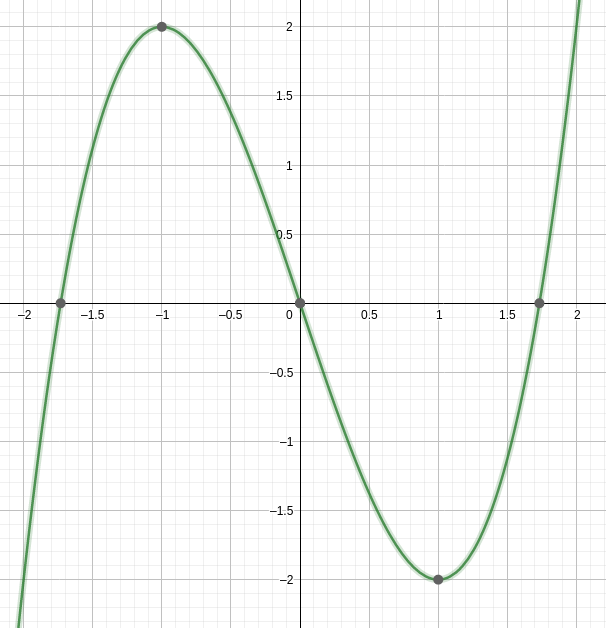
\includegraphics[width=0.4\textwidth]{fgv_elemzes}
\end{figure}
\vspace{30px}

\subsection{Alkalmazások}
\begin{itemize}
\item gazdasági problémák megoldása:
\begin{itemize}
\item Ha egy áru iránti kereslet függ a termék árától, akkor milyen ár esetén érhető el maximális összbevétel?
\item Ha egy termék előállítási költsége függ a termék reklámozására fordított összegtől, akkor mekkora reklámköltség esetén érhető el egy termék minimális előállítási költsége?
\end{itemize}
\item matematikai problémák megoldása:
\begin{itemize}
\item Adott térfogatú folyadéknak milyen méretekkel rendelkező hengeres dobozt tervezzünk, hogy a felhasznált csomagolóanyag mennyisége minimális legyen?
\item Adott sugarú gömbbe írt hengerek közül melyiknek a térfogata maximális?
\item Adott alapkörsugarú és magasságú forgáskúpba olyan forgáshengert írunk, amelynek alapköre a kúp alapkörének része, fedőköre pedig illeszkedik a kúp palástjára. Milyen esetben lesz a henger térfogata maximális?
\end{itemize}
\end{itemize}
\newpage







\section{Derékszögű háromszögekre vonatkozó tételek. A hegyesszögek szögfüggvényei. Összefüggések a hegyesszögek szögfüggvényei között. A szögfüggvények általánosítása}

\subsection{Derékszögű háromszögekre vonatkozó tételek}
\begin{definition}
Azokat a háromszögeket, amelyeknek valamely szöge 90$^\circ$, azaz derékszög, \textbf{derékszögű háromszög}eknek nevezzük.

A derékszöget bezáró két oldalt befogónak, a derékszöggel szemközti, egyben a leghosszabb oldalt átfogónak nevezzük.
\end{definition}

A derékszögű háromszögekre vonatkozó tételek közül a Pitagorasz-tétel teremt kapcsolatot a háromszög oldalai között.

\begin{theorem}[\textbf{Pitagorasz-tétel}]
Ha egy háromszög derékszögű, akkor befogóinak négyzetösszege egyenlő az átfogó négyzetével.
\end{theorem}
\begin{theorem}[\textbf{A Pitagorasz-tétel megfordítása}]
Ha egy háromszög két oldalhosszának négyzetösszege egyenlő a harmadik oldal hosszának négyzetével, akkor a háromszög derékszögű.
\end{theorem}
\begin{theorem}[\textbf{Thalész-tétel}]
Ha egy kör átmérőjének két végpontját összekötjük a kör bármely más pontjával, akkor derékszögű háromszöget kapunk.
\end{theorem}
\begin{proof}
$O$ középpontú kör, $AB$ átmérő, $C$ tetszőleges pont a körvonalon.
\begin{figure}[h]
\centering
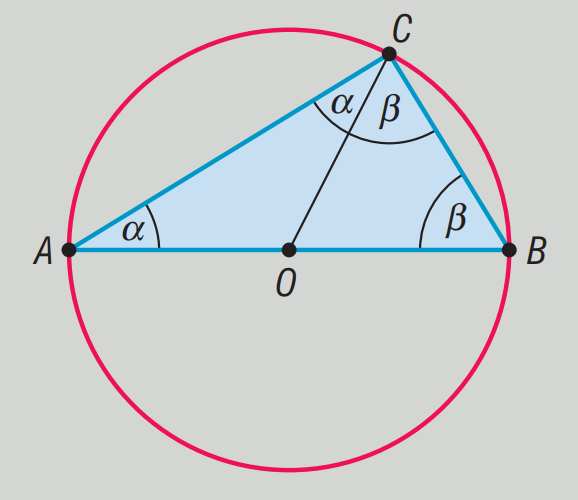
\includegraphics[scale=0.3]{geometry/thales}
\end{figure}

$OA = OC = r \Rightarrow$ Az $OAC$ háromszög egyenlő szárú $\Rightarrow OAC\sphericalangle = OCA\sphericalangle = \alpha$.

$OC = OB = r \Rightarrow$ Az $OBC$ háromszög egyenlő szárú $\Rightarrow OBC\sphericalangle = BCO\sphericalangle = \beta$.

Az $ABC$ háromszög belső szögeinek összege 180$^\circ \Rightarrow 2\alpha+2\beta=180^\circ \Rightarrow \alpha+\beta = 90^\circ \Rightarrow ACB\sphericalangle = 90^\circ$
\end{proof}
\begin{theorem}[\textbf{Thalész-tétel megfordítása}]
Ha egy háromszög derékszögű, akkor köré írható körének középpontja az átfogó felezőpontja.
\end{theorem}
\begin{theorem}[\textbf{Thalész tétele és annak megfordítása}]
Azon pontok halmaza síkon, amelyekből a sík egy AB szakasza derékszögben látszik, az AB átmérőjű körvonal, kivéve az A és a B pontokat.
\end{theorem}
\begin{theorem}[\textbf{Magasságtétel}]
Derékszögű háromszögben az átfogóhoz tartozó magasság hossza mértani közepe azon két szakasz hosszának, amelyekre a magasság az átfogót osztja.
\end{theorem}
\begin{theorem}[\textbf{Befogótétel}]
Derékszögű háromszög befogójának hossza mértani közepe az átfogó és a befogó átfogóra eső merőleges vetülete hosszának.
\end{theorem}
\begin{theorem}[\textbf{Beírt kör sugarára vonatkozó tétel}]
Derékszögű háromszög átfogója a két befogó összegével és a beírt kör sugarával kifejezve: $c = a + b - 2r$.
\end{theorem}

\subsection{Hegyesszögek szögfüggvényeinek definíciója}
A hegyesszögek szögfüggvényeit derékszögű háromszögekkel is bevezethetjük. Kihasználjuk, hogy a két derékszögű háromszög hasonló, ha valamely hegyesszögük megegyezik. A hasonlóság következtében egy derékszögű háromszög oldalainak arányát a háromszög egyik hegyesszöge egyértelműen meghatározza. Erre a függvényszerű kapcsolatra vezetjük be a szögfüggvényeket:

\begin{definition}
Az $\alpha$ hegyesszöget tartalmazó tetszőleges derékszögű háromszögben

$\sin\alpha$ = az $\alpha$-val szemközti befogó hosszának és az átfogó hosszának hányadosa;

$\cos\alpha =$ az $\alpha$ melletti befogó hosszának és az átfogó hosszának a hányadosa;

$\tg \alpha =$ az $\alpha$-val szemközti befogó hosszának és az $\alpha$ melletti befogó hosszának a hányadosa;

$\ctg\alpha =$ az $\alpha$ melletti befogó hosszának és az $\alpha$-val szemköztes befogó hosszának a hányadosa.
\begin{figure}[h]
\centering
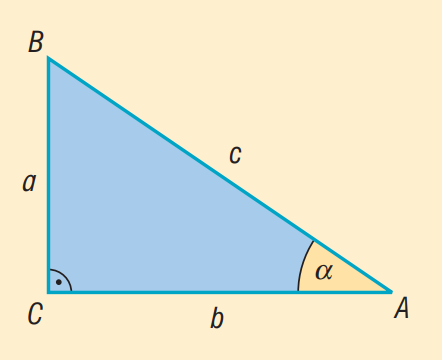
\includegraphics[scale=0.3]{geometry/derekszogu}
\end{figure}

\centering
$\sin\alpha=\dfrac{a}{c}, \cos\alpha=\dfrac{b}{c}, \tg\alpha=\dfrac{a}{b}, \ctg\alpha=\dfrac{b}{a}$
\end{definition}

\subsection{Összefüggések a hegyesszögek szögfüggvényei között}
A definíciók alapján könnyen igazolhatók a következő azonosságok, ahol $0^\circ<\alpha<90^\circ$:
\begin{center}
$\tg\alpha=\dfrac{\sin \alpha}{\cos \alpha}, \ctg\alpha=\dfrac{\cos \alpha}{\sin \alpha}, \tg\alpha=\dfrac{1}{\ctg \alpha}$

\[\sin \alpha = \cos (90^\circ-\alpha), \cos \alpha = \sin (90^\circ-\alpha)\]
\[\tg \alpha = \ctg (90^\circ-\alpha), \ctg \alpha = \tg (90^\circ-\alpha)\]
\[\sin^2\alpha + \cos^2\alpha = 1\]
\end{center}
\textbf{Nevezetes szögek szögfüggvényei:}
\begin{figure}[h]
\centering
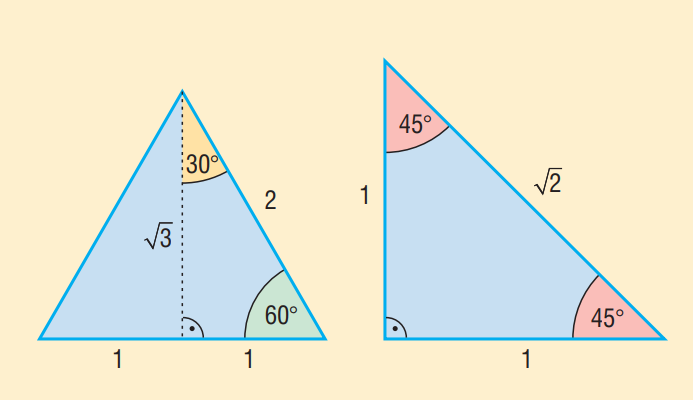
\includegraphics[scale=0.3]{geometry/hegyesszogfgv}
\end{figure}

\begin{center}
\begin{tabular}{c | c | c | c}
&$30^\circ$&$45^\circ$&$60^\circ$ \\
\hline
$\sin$ &$\dfrac{1}{2}$&$\dfrac{\sqrt{2}}{2}$&$\dfrac{\sqrt{3}}{2}$ \\[15pt] \hline
$\cos$ &$\dfrac{\sqrt{3}}{2}$&$\dfrac{\sqrt{2}}{2}$&$\dfrac{1}{2}$ \\[15pt] \hline
$\tg$ &$\dfrac{\sqrt{3}}{3}$&$1$&$\sqrt{3}$ \\[15pt] \hline
$\ctg$ &$\sqrt{3}$&$1$&$\dfrac{\sqrt{3}}{3}$
\end{tabular}
\end{center}

\subsection{Szögfüggvények általánosítása}

\begin{definition}
A \textbf{koordináta-rendszer}ben az $\vec{i}$(1; 0) bázisvektor origó körüli $\alpha$ szöggel való elforgatásával keletkező $\vec{e}$ egységvektor első koordinátája az $\alpha$ \textbf{szög koszinusza}, második koordinátája az $\alpha$ \textbf{szög szinusza}.
\end{definition}

\begin{center}
\begin{tabular}{c | c | c | c}
$\alpha \in I.$&$\alpha \in II.$&$\alpha \in III.$&$\alpha \in IV.$ \\[10pt]
\hline
$0<\alpha<\dfrac{\pi}{2}$&$\dfrac{\pi}{2}<\alpha<\pi$&$\pi<\alpha<\dfrac{3\pi}{2}$&$\dfrac{3\pi}{2}<\alpha<2\pi$ \\ \hline
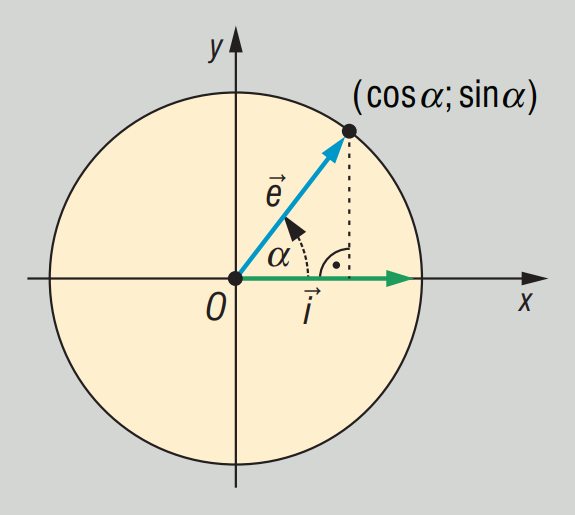
\includegraphics[scale=0.2]{geometry/forgasszog1}&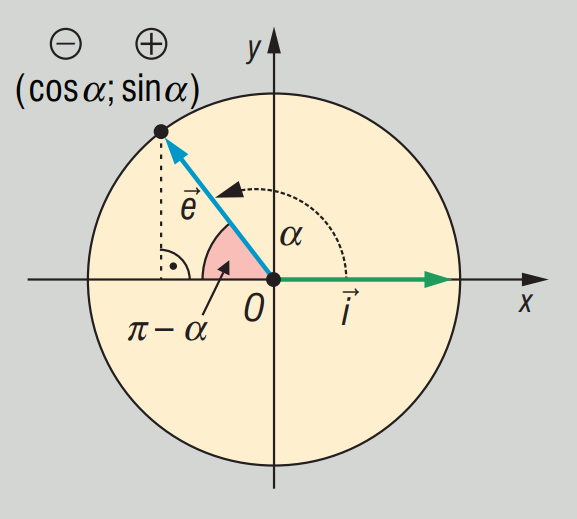
\includegraphics[scale=0.2]{geometry/forgasszog2}&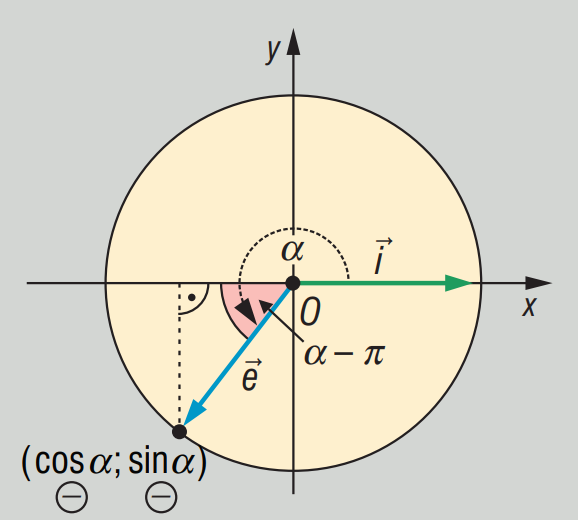
\includegraphics[scale=0.2]{geometry/forgasszog3}&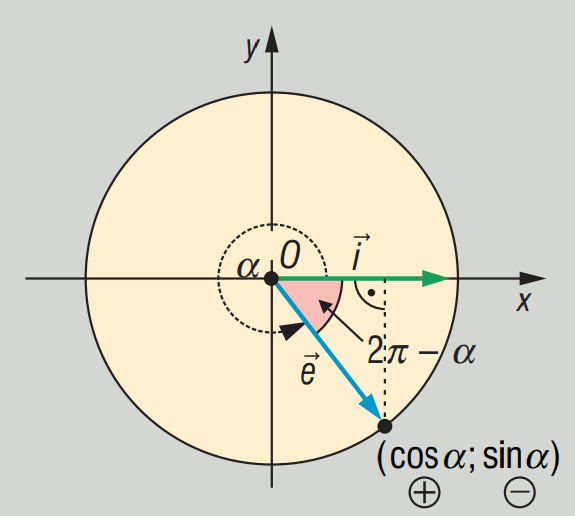
\includegraphics[scale=0.2]{geometry/forgasszog4} \\ \hline
&$\cos \alpha = -\cos(\pi-\alpha)$&$\cos \alpha = -\cos(\alpha-\pi)$&$\cos \alpha = \cos(2\pi-\alpha)$\\
&$\sin \alpha = \sin(\pi-\alpha)$&$\sin \alpha = -\sin(\alpha-\pi)$&$\sin \alpha = -\sin(2\pi-\alpha)$
\end{tabular}
\end{center}

\begin{definition}
A $\dfrac{\sin \alpha}{\cos \alpha}$ hányadost, ha $\cos \alpha \neq 0$, vagyis ha $\alpha \neq \dfrac{\pi}{2}+k\pi (k \in \mathbb{Z})$, az $\alpha$ szög tangensének nevezzük.

A \textbf{koordináta-rendszerben} az $\vec{i}$ vektortól $\alpha$ szöggel elforgatott $\vec{e}$ egységvektor egyenese által az origó középpontú, egységsugarú kör (1; 0) pontjában húzott érintőből kimetszett pont
2. koordinátája az $\alpha$ \textbf{szög tangense}.
\end{definition}

\begin{center}
\begin{tabular}{c | c | c | c}
$\alpha \in I.$&$\alpha \in II.$&$\alpha \in III.$&$\alpha \in IV.$ \\[10pt]
\hline
$0<\alpha<\dfrac{\pi}{2}$&$\dfrac{\pi}{2}<\alpha<\pi$&$\pi<\alpha<\dfrac{3\pi}{2}$&$\dfrac{3\pi}{2}<\alpha<2\pi$ \\ \hline
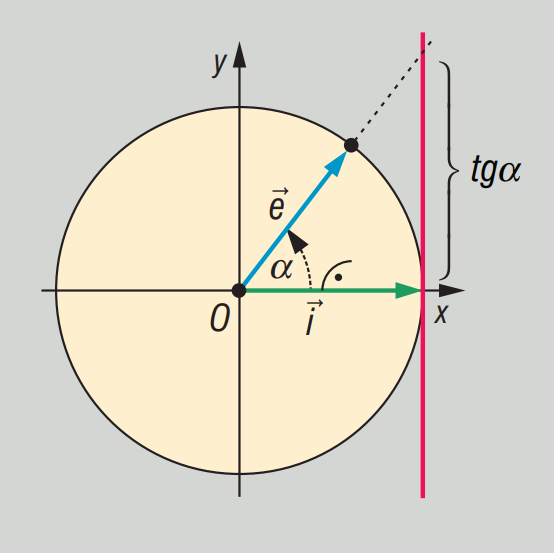
\includegraphics[scale=0.2]{geometry/forgasszog5}&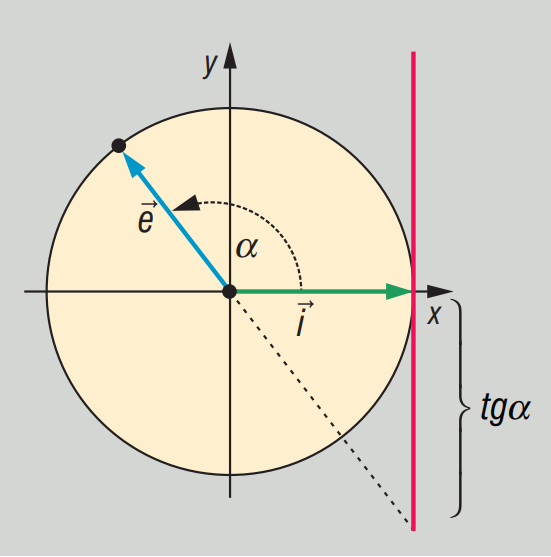
\includegraphics[scale=0.2]{geometry/forgasszog6}&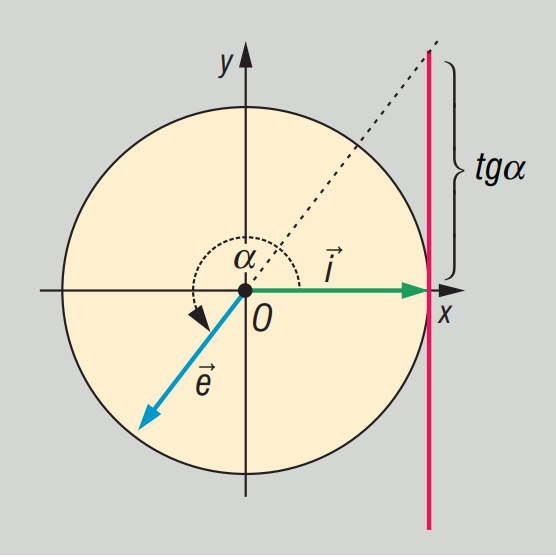
\includegraphics[scale=0.2]{geometry/forgasszog7}&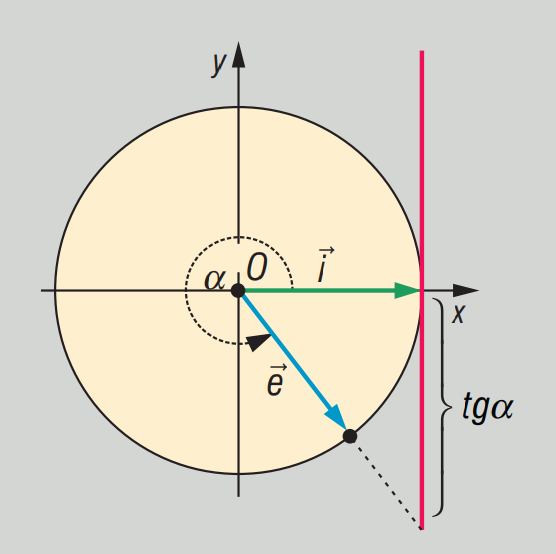
\includegraphics[scale=0.2]{geometry/forgasszog8} \\ \hline
&$\tg \alpha = -\tg(\pi-\alpha)$&$\tg \alpha = \tg(\alpha-\pi)$&$\tg \alpha = -\tg(2\pi-\alpha)$\\
\end{tabular}
\end{center}

\begin{definition}
A $\dfrac{\cos \alpha}{\sin \alpha}$ hányadost, ha $\sin \alpha \neq 0$, vagyis ha $\alpha \neq k\pi (k \in \mathbb{Z})$, az $\alpha$ szög kotangensének nevezzük.

A \textbf{koordináta-rendszerben} az $\vec{i}$ vektortól $\alpha$ szöggel elforgatott $\vec{e}$ egységvektor egyenese által az origó középpontú, egységsugarú kör (0; 1) pontjában húzott érintőből kimetszett pont 1. koordinátája az $\alpha$ \textbf{szög kotangense}.
\end{definition}

\begin{center}
\begin{tabular}{c | c | c | c}
$\alpha \in I.$&$\alpha \in II.$&$\alpha \in III.$&$\alpha \in IV.$ \\[10pt]
\hline
$0<\alpha<\dfrac{\pi}{2}$&$\dfrac{\pi}{2}<\alpha<\pi$&$\pi<\alpha<\dfrac{3\pi}{2}$&$\dfrac{3\pi}{2}<\alpha<2\pi$ \\ \hline
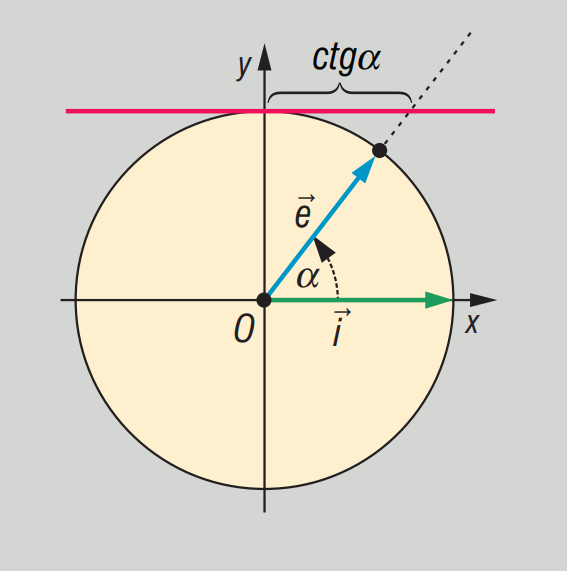
\includegraphics[scale=0.2]{geometry/forgasszog9}&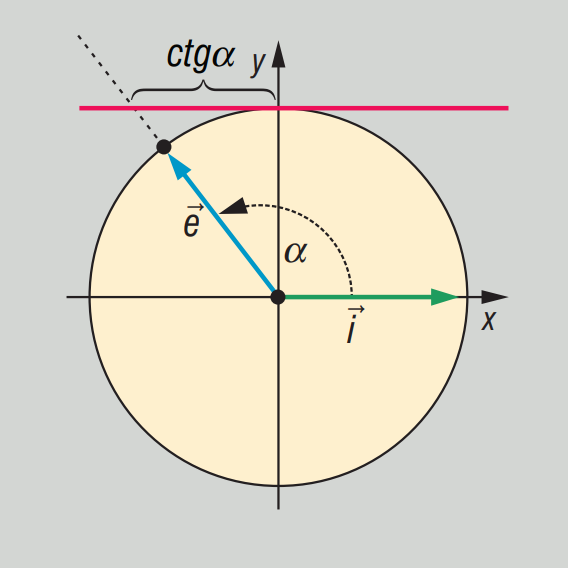
\includegraphics[scale=0.2]{geometry/forgasszog10}&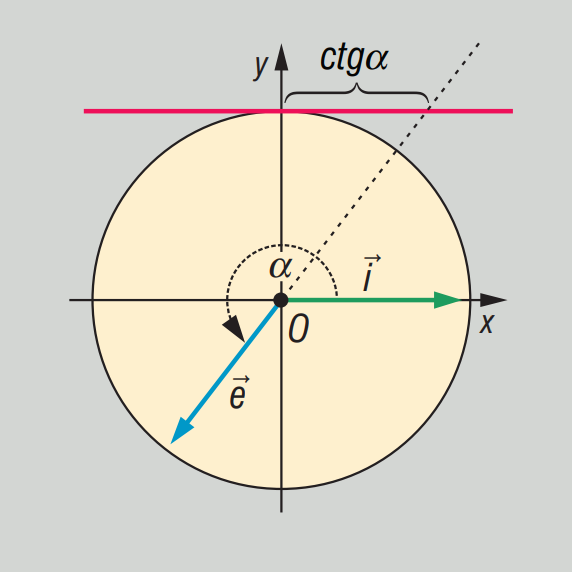
\includegraphics[scale=0.2]{geometry/forgasszog11}&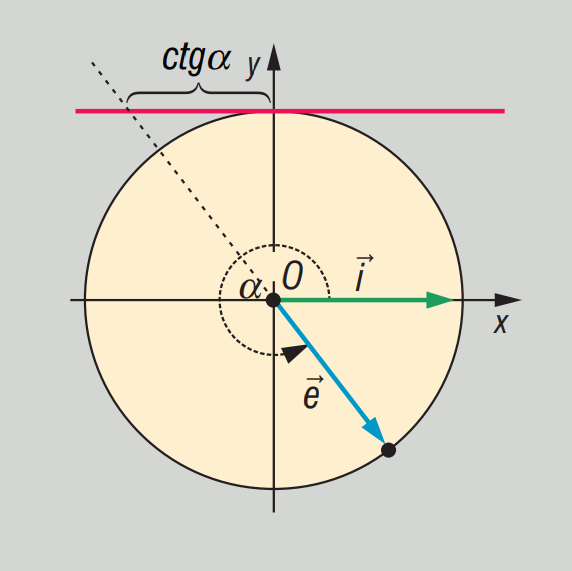
\includegraphics[scale=0.2]{geometry/forgasszog12} \\ \hline
&$\ctg \alpha = -\ctg(\pi-\alpha)$&$\ctg \alpha = \ctg(\alpha-\pi)$&$\ctg \alpha = -\ctg(2\pi-\alpha)$\\
\end{tabular}
\end{center}

\subsection{Kapcsolatok egyazon szög szögfüggvényei között}

\begin{theorem}
\[\ctg\alpha=\dfrac{1}{\tg\alpha}\text{, ha }\alpha\neq k\dfrac{\pi}{2}(k\in\mathbb{Z})\]
\[\tg\alpha=\dfrac{1}{\ctg\alpha}\text{, ha }\alpha\neq k\dfrac{\pi}{2}(k\in\mathbb{Z})\]
\[\Rightarrow  \tg\alpha\cdot\ctg \alpha=1\left(\alpha\neq k\dfrac{\pi}{2}(k\in\mathbb{Z})\right)\]
\end{theorem}

\begin{theorem}[Pitagoraszi összefüggés]
$\sin^2\alpha+\cos^2\alpha=1$ minden valós $\alpha$-ra.
\end{theorem}
\textbf{Következmény:}
\[|\sin \alpha|=\sqrt{1-\cos^2\alpha}\]
\[|\cos \alpha|=\sqrt{1-\sin^2\alpha}\]

\subsection{Alkalmazások}
\begin{itemize}
\item Pitagorasz-tétel: síkgeometria: háromszög, trapéz magasságának számolása, koordinátageometria: két pont távolsága, vektor hossza
\item Thalész-tétel: síkgeometria: körhöz külső pontból húzott érintők szerkesztése, koordinátageometria: érintők egyenlete
\item Forgásszögek szögfüggvényei: háromszög trigonometrikus területképlete, szinusztétel, koszinusztétel, rezgőmozgás kitérés-idő, sebesség-idő, gyorsulás-idő függvénye trigonometrikus függvény
\end{itemize}
\newpage






\section{Háromszögek nevezetes vonalai, pontjai és körei}

\subsection{Oldalfelező merőlegesek, a háromszög köré írt kör középpontja}
\begin{definition}
A síkon egy \textbf{szakasz felezőmerőlegese} az az egyenes, amely a szakasz felezőpontjára illeszkedik és merőleges a szakaszra.
\end{definition}

\begin{theorem}
A szakasz felezőmerőlegese a szakasz két végpontjától egyenlő távol lévő pontok halmaza.
\end{theorem}

\begin{theorem}
A háromszög három oldalfelező merőlegese egy pontban metszi egymást. Ez a pont a \textbf{háromszög köré írt kör középpontja}.
\end{theorem}
\begin{proof}
$ABC$ háromszögben $AB$ és $AC$ oldalfelező merőlegeseit tekintsük. Ezek az egyenesek metszik egymást, mert a háromszög oldalai nem párhuzamosak egymással. Legyen a két oldalfelező merőleges metszéspontja $K$. Ekkor $K$ egyenlő távolságra van $A$-tól és $B$-től (mert $K$ illeszkedik $f_c$-re), illetve $A$-tól és $C$-től (mert $K$ illeszkedik $f_b$-re) is. Következésképpen egyenlő távol van $B$-től és $C$-től is, azaz $K$ illeszkedik $BC$ szakaszfelező merőlegesére. $\Rightarrow KA = KB = KC$, azaz $A$, $B$ és $C$ egyenlő távolságra vannak $K$-tól $\Rightarrow$ mindhárom pont illeszkedik egy $K$ középpontú $KA = KB = KC = r$ sugarú körre.
\begin{figure}[h]
\centering
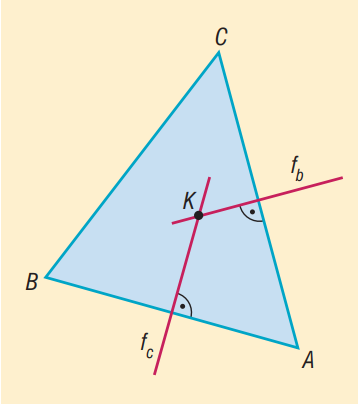
\includegraphics[scale=0.4]{geometry/korul_irt_kor}
\end{figure}

\end{proof}

$K$ hegyesszögű háromszög esetén a háromszögön belül, derékszögű háromszögnél az átfogó felezőpontjába (Thalész tétele), tompaszögű háromszögnél a háromszögön kívül esik.
\begin{figure}[h]
\centering
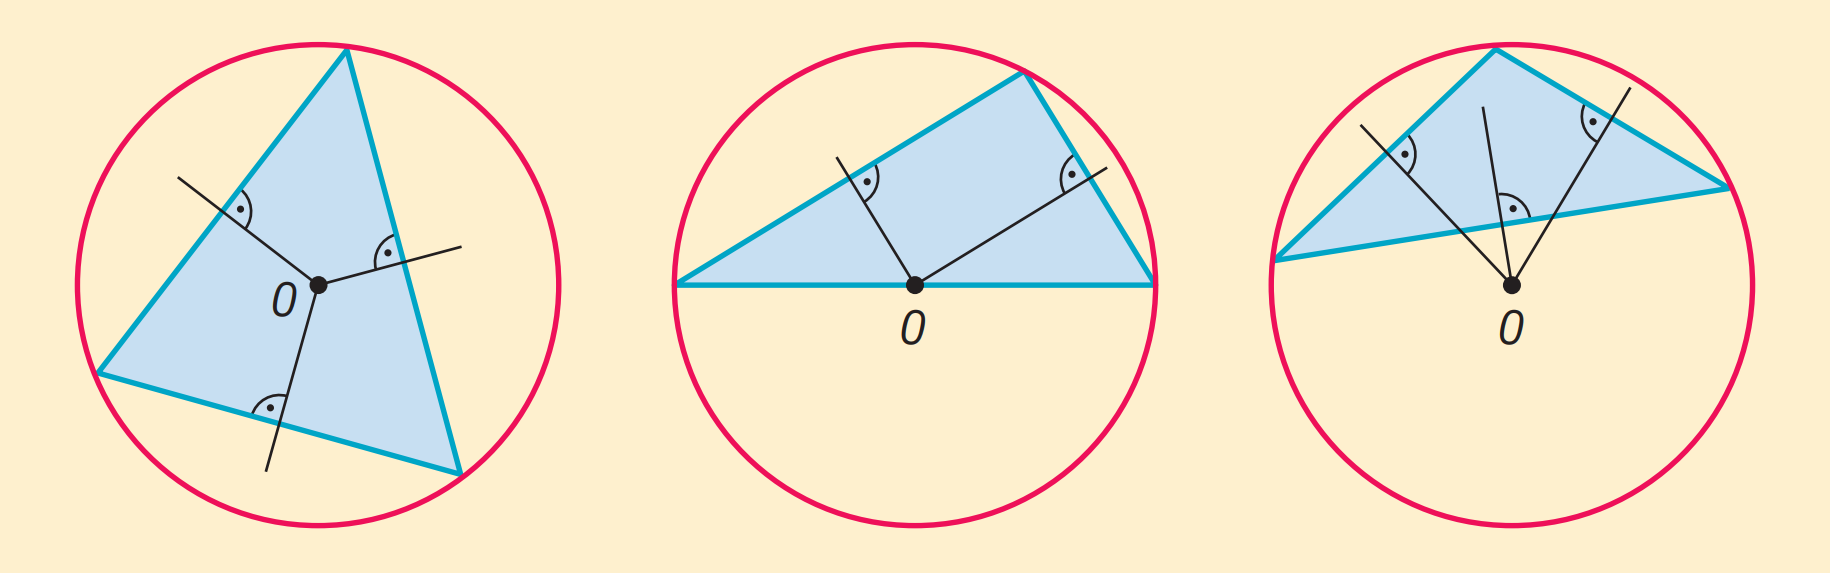
\includegraphics[scale=0.2]{geometry/korul_irt_kor_esetek}
\end{figure}
\newpage
\subsection{Szögfelezők, háromszögbe, illetve háromszöghöz írt kör középpontja}

\begin{definition}
Egy konvex szög \textbf{szögfelező}je a szög csúcsából kiinduló, a szögtartományban haladó azon félegyenes, amely a szöget két egyenlő nagyságú szögre bontja.
\end{definition}

\begin{theorem}
Egy konvex szögtartományban a száraktól egyenlő távolságra lévő pontok halmaza a szögfelező.
\end{theorem}

\begin{theorem}
A háromszög három belső szögfelezője egy pontban metszi egymást. Ez a pont a \textbf{háromszögbe írt kör középpontja}.
\end{theorem}

\begin{theorem}
A háromszög egy belső, és a másik két csúcshoz tartozó külső szögfelezője egy pontban metszi egymást, ez a pont a \textbf{háromszög hozzáírt körének középpontja}. A háromszögnek 3 hozzáírt köre van.
\begin{figure}[h]
\centering
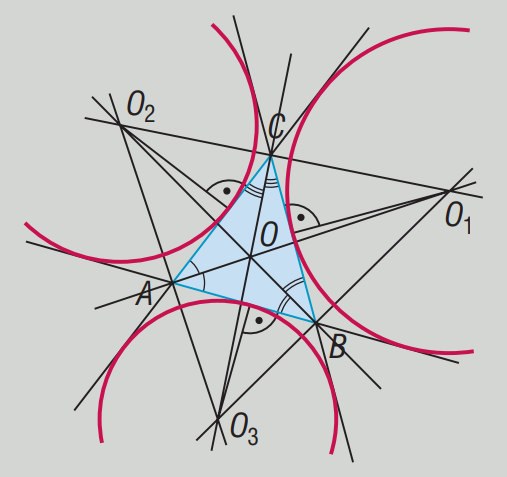
\includegraphics[scale=0.3]{geometry/hozzairt_kor}
\end{figure}

\end{theorem}

\begin{theorem}
A háromszög ugyanazon szögének külső és belső szögfelezője merőleges egymásra.
\end{theorem}

\subsection{Magasságvonalak, a háromszög magasságpontja}

\begin{definition}
A háromszög \textbf{magasság}a az egyik csúcsból a szemközti oldal egyenesére bocsátott merőleges szakasz. A háromszög magasságának egyenese a háromszög \textbf{magasságvonal}a.
\end{definition}

\begin{theorem}
A háromszög magasságvonalai egy pontban metszik egymást. Ez a pont a háromszög \textbf{magasságpont}ja.
\end{theorem}

A magasságpont hegyesszögű háromszög esetén a háromszög belsejében, derékszögű háromszögnél a derékszögű csúcsban, tompaszögű háromszögnél a háromszögön kívül helyezkedik el.
\begin{figure}[h]
\centering
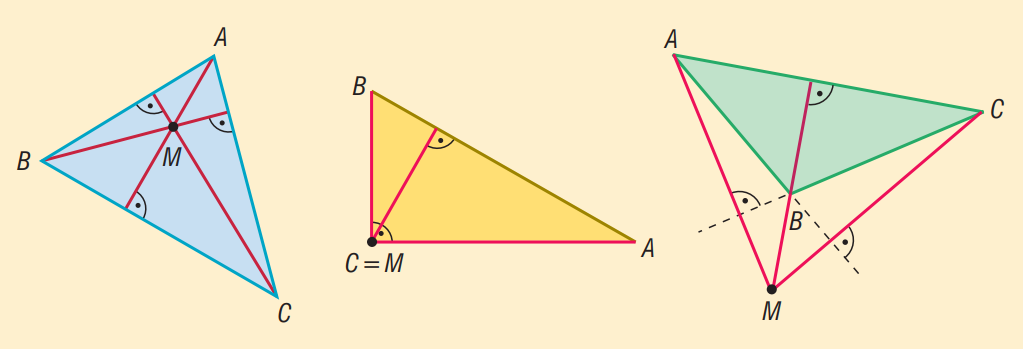
\includegraphics[scale=0.3]{geometry/magassagpont}
\end{figure}
\newpage
\subsection{Súlyvonalak, a háromszög súlypontja}

\begin{definition}
A háromszög csúcsát a szemközti oldal felezőpontjával összekötő szakasz a \textbf{háromszög súlyvonala}.
\end{definition}

\begin{theorem}
A háromszög súlyvonalai egy pontban metszik egymást, ezt a pontot a háromszög \textbf{súlypont}jának nevezzük. A súlypont harmadolja a súlyvonalakat úgy, hogy a csúcs felé eső szakasz úgy aránylik az oldal felé eső szakaszhoz, mint 2 : 1.
\end{theorem}

\begin{figure}[h]
\centering
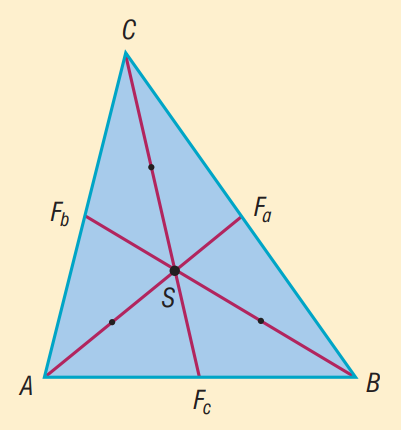
\includegraphics[scale=0.3]{geometry/sulypont}
\end{figure}

\subsection{Középvonalak}

\begin{definition}
A háromszög két oldalfelező pontját összekötő szakaszt a \textbf{háromszög középvonal}ának nevezzük.

Minden háromszögnek 3 középvonala van.
\end{definition}

\begin{theorem}
A háromszög középvonala párhuzamos a felezőpontokat nem tartalmazó oldallal, és fele olyan hosszú.
\end{theorem}
\begin{figure}[h]
\centering
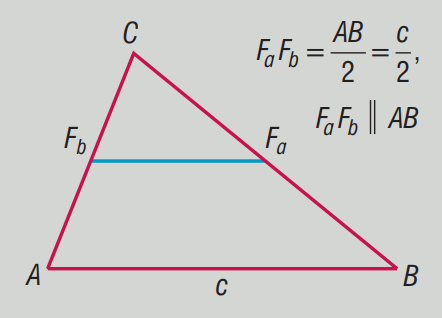
\includegraphics[scale=0.3]{geometry/kozepvonal}
\end{figure}
\newpage
\subsection{Euler-egyenes, Feuerbach-kör}

\begin{theorem}
A háromszög magasságpontja, súlypontja és a körülírt kör középpontja egy egyenesen van (\textbf{Euler-féle egyenes}). A súlypont a másik kettő távolságát harmadolja és a körülírt kör középpontjához van közelebb.
\begin{figure}[h]
\centering
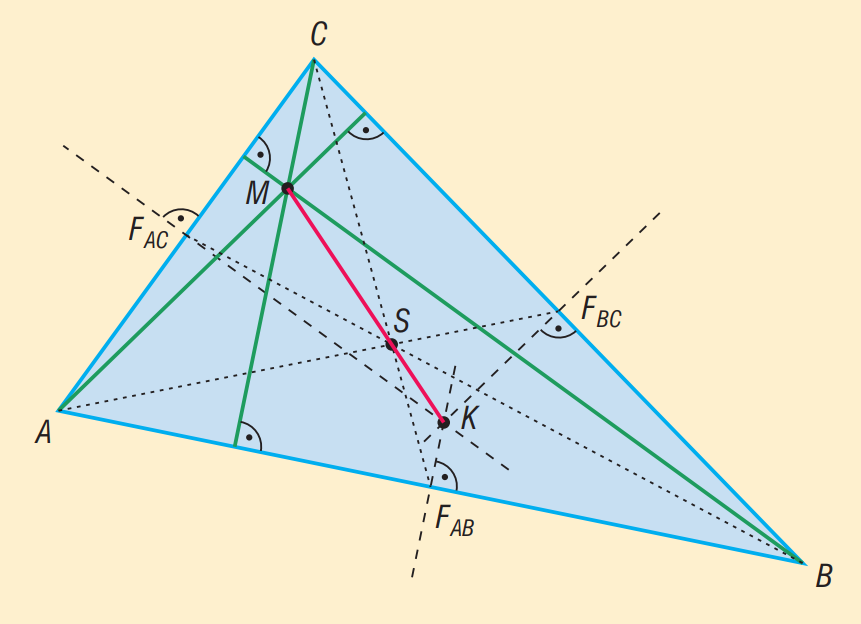
\includegraphics[scale=0.4]{geometry/euler_egyenes}
\end{figure}

\end{theorem}

\begin{theorem}
Egy háromszög oldalainak felezőpontjai, magasságainak talppontjai és a magasságpontot a csúcsokkal összekötő szakaszok felezőpontjai egy körön vannak (\textbf{Feuerbach-kör}).

A Feuerbach-kör középpontja ($O$) felezi a magasságpontot ($M$) és a köré írható kör középpontját ($K$) összekötő szakaszt, sugara a háromszög köré írható kör sugarának a fele. Vagyis az $M$ pontból a köré írt kör $\lambda = \dfrac{1}{2}$-es arányú kicsinyített képe a Feuerbach-kör.

\begin{figure}[h]
\centering
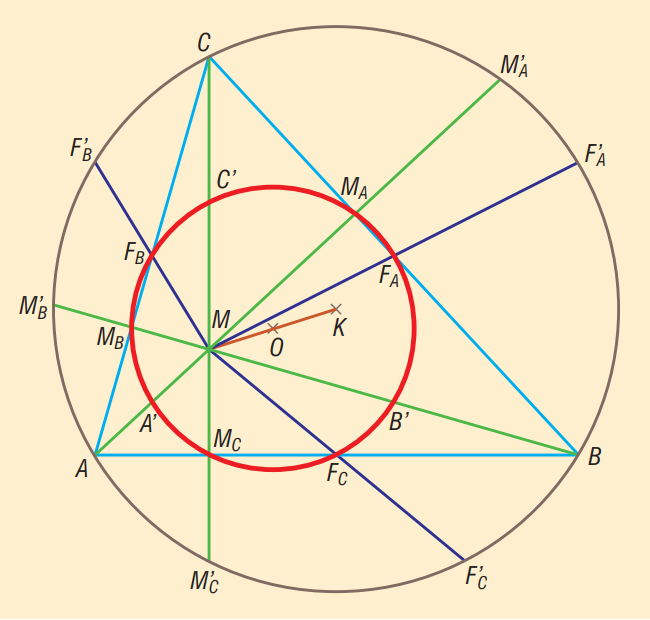
\includegraphics[scale=0.4]{geometry/feuerbach}
\end{figure}

\end{theorem}
\subsection{Alkalmazások}
\begin{itemize}
\item Háromszögszerkesztési feladatok
\item Koordináta-geometria: 3 ponton átmenő kör egyenlete, háromszög súlypontjának kiszámítása
\item Súlyvonal, súlypont (homogén anyageloszlású háromszög esetén) fizikában: súlyvonal mentén, illetve súlypontban alátámasztva a háromszög egyensúlyban van
\item Kör középpontjának szerkesztése
\item Területszámítási feladatok a nevezetes körök sugarainak felhasználásával
$$t=\dfrac{abc}{4R}$$
$$t=r\cdot s, \hspace{20px} \left(s=\dfrac{k}{2}\right)$$
\end{itemize}
\newpage





\section{Összefüggések az általános háromszögek oldalai között, szögei között, oldalai és szögei között}

\subsection{Háromszögek csoportosítása szögeik és oldalaik szerint}

\begin{definition}
\textbf{Háromszög} az a zárt szögvonal, amelyeknek 3 oldala és 3 csúcsa van.
\end{definition}

\begin{definition}
Egy háromszög \textbf{hegyesszögű}, ha minden szöge hegyesszög.
\end{definition}

\begin{definition}
Egy háromszög \textbf{derékszögű}, ha van egy $90^\circ$-os szöge.
\end{definition}

\begin{definition}
Egy háromszög \textbf{tompaszögű}, ha van egy tompaszöge.
\end{definition}

\begin{definition}
Egy háromszög \textbf{szabályos} (vagy egyenlő oldalú), ha három oldala egyenlő hosszú.
\end{definition}

\begin{definition}
Egy háromszög \textbf{egyenlő szárú} (vagy szimmetrikus), ha van két egyenlő oldala
\end{definition}

\begin{figure} [h]
\centering
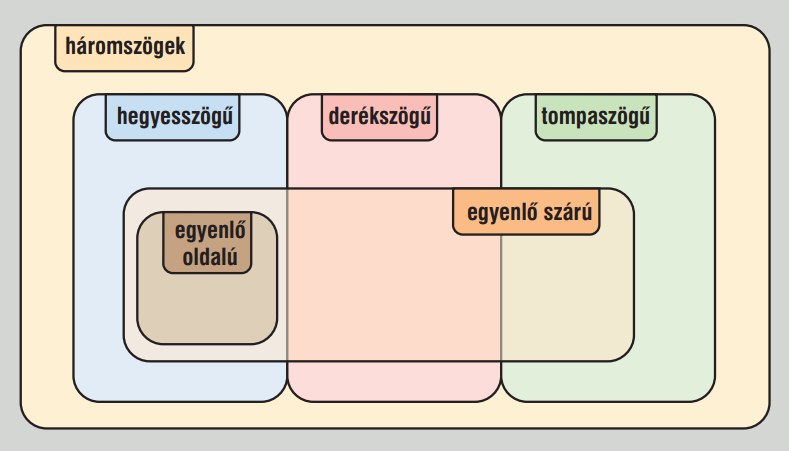
\includegraphics[scale=0.3]{geometry/haromszogek_csop}
\end{figure}

\subsection{Összefüggések a háromszög oldalai közt}

\begin{theorem}
Háromszög-egyenlőtlenségek: a háromszög bármely két oldalának összege nagyobb a harmadiknál: a + b > c, a + c > b, b + c > a.
\end{theorem}

\begin{theorem}
Egy háromszögben bármely két oldal különbségének abszolút értéke kisebb a harmadiknál: $|a - c|< b, |a - b|< c, |b - c|< a$.
\end{theorem}

\begin{theorem}
Pitagorasz-tétel: Bármely derékszögű háromszögben a két befogó négyzetének összege egyenlő az átfogó négyzetével.
\end{theorem}

\subsection{Összefüggések a háromszög szögei közt}

\begin{theorem}
A háromszög belső szögeinek összege $180^\circ$.
\end{theorem}

\begin{theorem}
A háromszög külső szögeinek összege $360^\circ$.
\end{theorem}

\begin{theorem}
A háromszög egy külső szöge egyenlő a nem mellette fekvő két belső szög összegével.
\end{theorem}
\newpage
\subsection{Összefüggések a háromszög oldalai és szögei között}

\begin{theorem}
Egy háromszögben egyenlő hosszúságú oldalakkal szemben egyenlő nagyságú szögek vannak, egyenlő nagyságú szögekkel szemben egyenlő hosszúságú oldalak vannak.
\end{theorem}

\begin{theorem}
Bármely háromszögben két oldal közül a hosszabbikkal szemben nagyobb belső szög van, mint a rövidebbikkel szemben, illetve két szög közül a nagyobbikkal szemben hosszabb oldal van, mint a kisebbikkel szemben.
\end{theorem}

\begin{definition}
Derékszögű háromszögben bevezetjük a \textbf{szögfüggvények} fogalmát a hasonló háromszögek tulajdonságait kihasználva:

$\sin\alpha$ = az $\alpha$-val szemközti befogó hosszának és az átfogó hosszának hányadosa;

$\cos\alpha =$ az $\alpha$ melletti befogó hosszának és az átfogó hosszának a hányadosa;

$\tg \alpha =$ az $\alpha$-val szemközti befogó hosszának és az $\alpha$ melletti befogó hosszának a hányadosa;

$\ctg\alpha =$ az $\alpha$ melletti befogó hosszának és az $\alpha$-val szemköztes befogó hosszának a hányadosa.
\begin{figure}[h]
\centering
\includegraphics[scale=0.3]{geometry/derekszogu}
\end{figure}

\centering
$\sin\alpha=\dfrac{a}{c}, \cos\alpha=\dfrac{b}{c}, \tg\alpha=\dfrac{a}{b}, \ctg\alpha=\dfrac{b}{a}$
\end{definition}

\begin{theorem} [\textbf{Szinusztétel}]
Egy háromszögben két oldal hosszának aránya egyenlő a velük szemközti szögek szinuszának arányával:
$$\dfrac{a}{b}=\dfrac{\sin \alpha}{\sin \beta}$$
A szinusztétel a háromszög három oldalára is felírható, ekkor $a : b : c = \sin \alpha : \sin \beta : \sin \gamma$.
\end{theorem}

\textbf{Szinusztétel alkalmazása:}

\begin{itemize}
\item  Ha adott a háromszög egy oldala és két szöge, akkor bármely oldal kiszámolható (mert ekkor kiszámolható a belső szögösszegből a harmadik szög).
\item Ha adott a háromszög két oldala és nem az általuk közbezárt szög ismert, akkor két eset lehetségséges:
\begin{itemize}
\item  Ha a két oldal közül a nagyobbikkal szemköztes szög ismert, akkor kiszámolható a kisebbik oldallal szemköztes szög. Ebben az esetben a háromszög egyértelműen meghatározott.
\item Ha a háromszög két oldalát és a rövidebbel szemköztes szöget ismerjük, akkor kiszámolható a nagyobbik oldallal szemköztes szög, amire háromféle megoldás is lehet:
\begin{enumerate}
\item ha a szög szinuszára pozitív, de 1-nél kisebb értéket kapunk, akkor két megoldás van, a szög lehet hegyesszög és tompaszög is. Ekkor a háromszög nem egyértelműen meghatározott, két ilyen háromszög létezik.
\item ha a szög szinuszára 1-et kapunk, akkor egy megoldás van, a szög $90^\circ$, ez egy derékszögű háromszög.
\item  ha a szög szinuszára 1-nél nagyobb számot kapunk, akkor nincs ilyen szög, azaz nincs az adatoknak megfelelő háromszög.
\end{enumerate}
\end{itemize}
\end{itemize}

Ebben az esetben inkább a koszinusztételt alkalmazzuk, ekkor másodfokú egyenletet kapunk a harmadik oldalra, így viszont egyértelműen eldönthető az oldal hossza (a másodfokú egyenletnek 0, 1, 2 megoldása van, illetve feltétel, hogy az oldal hossza pozitív, vagy a háromszög-egyenlőtlenség is segíthet abban, hogy eldöntsük, hogy melyik eredmény megoldása a feladatnak).

\begin{theorem} [\textbf{Koszinusztétel}]
egy háromszög egyik oldalhosszának négyzetét megkapjuk, ha a másik két oldal négyzetösszegéből kivonjuk a két oldal hosszának és a közbezárt szög koszinuszának kétszeres szorzatát: $c^2=a^2+b^2-2ab\cos \gamma$.
\end{theorem}
\begin{proof}
Vektorok skaláris szorzatának felhasználásával fogjuk bizonyítani, ezért a háromszög oldalait irányítjuk:
$$\overrightarrow{CB}=\vec{a}, \hspace{10px} \overrightarrow{CA}=\vec{b}, \hspace{10px} \overrightarrow{BA}=\vec{c}.$$
Jelölje: $|\vec{a}|=a, \hspace{10px} |\vec{b}| = b, \hspace{10px} |\vec{c}| = c$
\begin{figure}[h]
\centering
\includegraphics[scale=0.3]{geometry/koszinusztetel}
\end{figure}

Ekkor $\vec{c}=\vec{b}-\vec{a}$. Az egyenlet mindkét oldalát önmagával skalárisan szorozva:

$$(\vec{c})^2=(\vec{b}-\vec{a})^2 \Rightarrow (\vec{c})^2 = (\vec{a})^2 - 2\vec{a}\vec{b}+ (\vec{b})^2$$
$$(\vec{c})^2=|\vec{c}|\cdot |\vec{c}| \cdot \cos 0^\circ = c\cdot c \cdot 1= c^2$$
Hasonlóan: $(\vec{a})^2=a^2$ és $(\vec{b})^2=b^2$
$$\vec{a}\cdot \vec{b}=|\vec{a}|\cdot |\vec{b}|\cdot \cos \gamma= a\cdot b\cdot \cos \gamma$$
Ezeket beírva a $(\vec{c})^2 = (\vec{a})^2 - 2\vec{a}\vec{b}+ (\vec{b})^2$ egyenletbe kapjuk: $c^2=a^2+b^2-2ab\cos \gamma$
\end{proof}
\textbf{Következmények:}
\begin{itemize}
\item ha $\gamma = 90^\circ$, vagyis a háromszög derékszögű, akkor $c^2 = a^2 + b^2$, ami a Pitagorasz-tétel.
\item  ha $\gamma < 90^\circ$, akkor bármely két oldalának négyzetösszege nagyobb a harmadik oldal négyzeténél.
\item ha $\gamma > 90^\circ$, akkor a két rövidebb oldal négyzetösszege kisebb a harmadik oldal négyzeténél.
\end{itemize}
\newpage
\textbf{Koszinusztétel alkalmazása:}
\begin{itemize}
\item Ha adott a háromszög két oldala és az általuk közbezárt szög, akkor kiszámítható a szöggel szembeni oldal.
\item  Ha adott a háromszög három oldala, akkor kiszámolható a háromszög bármely szöge. 

Ha keressük a háromszög szögeit, akkor ebben az esetben a háromszög legnagyobb szögét érdemes kiszámolni koszinusztétellel, ami a leghosszabb oldallal szemben van, mert az hegyes-, derék- és tompaszögre is egyértelmű megoldást ad.
\end{itemize}

\subsection{Alkalmazások}
\begin{itemize}
\item Háromszögek szerkesztése, háromszög ismeretlen adatainak kiszámítása
\item Sokszögekben oldalak, átlók, szögek kiszámolása háromszögekre bontással
\item Földmérésben, térképészetben, csillagászatban mért adatokból távolságok és szögek kiszámolása
\item  Terepfeladatok megoldásánál: pl.: megközelíthetetlen pontok helyének meghatározása
\item  Modern helymeghatározás: GPS
\end{itemize}
\newpage





\section{Egybevágósági transzformációk, alakzatok egybevágósága. Szimmetria. Hasonlósági transzformációk. Hasonló síkidomok kerülete, területe, hasonló testek felszíne, térfogata. A hasonlóság alkalmazásai síkgeometriai tételek bizonyításában}

\subsection{Transzformációk}

\begin{definition}
\textbf{Geometriai transzformációk} azok a függvények, amelyek egy ponthalmazt ponthalmazra képeznek le. ($D_f=R_f=$ ponthalmaz)
\end{definition}

\begin{definition}
A geometriai transzformációk közül a távolságtartó transzformációkat \textbf{egybevágósági transzformációknak} nevezzük.

Távolságtartó leképezés: bármely két pont távolsága egyenlő képeik távolságával.

Síkbeli egybevágósági transzformációk: tengelyes tükrözés, pontra vonatkozó (középpontos) tükrözés, pont körüli elforgatás, eltolás, és ezek egymás utáni alkalmazása.
\end{definition}

\begin{definition}
\textbf{Tengelyes tükrözés}: adott a sík egy ``t'' egyenese, ez a tengelyes tükrözés tengelye. A ``t'' tengelyre vonatkozó tengelyes tükrözés a sík tetszőleges ``t''-re nem illeszkedő ``P'' pontjához azt a P' pontot rendeli, amelyre fennáll, hogy a PP' szakasz felezőmerőlegese a ``t'' tengely. A ``t'' egyenes képe önmaga.
\begin{figure}[h!]
\centering
\includegraphics[scale=0.3]{geometry/tengelyes_tukr}
\end{figure}
\end{definition}

\begin{definition}
\textbf{Középpontos tükrözés}: adott a sík egy ``O'' pontja, a középpontos tükrözés középpontja. Az ``O'' pontra vonatkozó középpontos tükrözés a sík egy tetszőleges ``O''-tól különböző ``P'' pontjához azt a P' pontot rendeli, amelyre az ``O'' pont a PP' szakasz felezőpontja. Az ``O'' pont képe önmaga.
\begin{figure}[h!]
\centering
\includegraphics[scale=0.3]{geometry/kp_tukr}
\end{figure}
\end{definition}
\newpage
\begin{definition}
\textbf{Pont körüli forgatás}: adott a sík egy ``O'' pontja és egy $\alpha$ irányított szög. Az ``O'' pont körüli $\alpha$ szögű, adott irányú forgatás a sík egy tetszőleges ``O''-tól különböző ``P'' pontjához azt a P' pontot rendeli, amelyre teljesül, hogy POP' szög irány és nagyság szerint megegyezik $\alpha$-val és OP = OP'. ``O'' pont képe önmaga.
\begin{figure}[h!]
\centering
\includegraphics[scale=0.3]{geometry/forg}
\end{figure}
\end{definition}

\begin{definition}
\textbf{Eltolás}: adott egy $\vec{v}$ vektor. A $\vec{v}$ vektorral való eltolás a sík (tér) tetszőleges ``P'' pontjához azt a P' pontot rendeli, amelyre $\overrightarrow{PP'}$ = $\vec{v}$.
\begin{figure}[h!]
\centering
\includegraphics[scale=0.3]{geometry/eltolas}
\end{figure}
\end{definition}

\subsection{Alakzatok egybevágósága (háromszögek, sokszögek)}

\begin{definition}
Két alakzat egybevágó, ha van olyan egybevágósági transzformáció, amely az egyik alakzatot a másikba viszi. Jele: $A \cong B$.
\end{definition}

\begin{theorem}
Két háromszög akkor és csak akkor egybevágó, ha:
\begin{itemize}
\item megfelelő oldalaik hossza páronként egyenlő,
\item két-két oldaluk hossza páronként egyenlő és az ezek által közbezárt szögek nagysága egyenlő,
\item két-két oldaluk hossza páronként egyenlő és e két-két oldal közül a hosszabbikkal szemközti szögük nagysága egyenlő,
\item egy-egy oldaluk hossza páronként egyenlő és két-két szögük páronként egyenlő.
\end{itemize}
\end{theorem}

\begin{theorem}
Két sokszög akkor és csak akkor egybevágó, ha a következő feltételek egyike teljesül:
\begin{itemize}
\item megfelelő oldalaik hossza és a megfelelő átlóik hossza páronként egyenlő,
\item megfelelő oldalaik hossza páronként egyenlő és megfelelő szögeik páronként egyenlők.
\end{itemize}
\end{theorem}

\subsection{Szimmetria}

\begin{definition}
Ha egy ponthalmazhoz található olyan ``t'' egyenes, amelyre vonatkozó tükörképe önmaga, akkor ez a ponthalmaz \textbf{tengelyesen szimmetrikus}, amelynek ``t'' a szimmetriatengelye. Tengelyesen szimmetrikus síkidomok: egyenlő szárú háromszög, egyenlő oldalú háromszög, deltoid, húrtrapéz, rombusz, téglalap, négyzet, szabályos sokszögek, kör
\end{definition}

\begin{definition}
Ha egy ponthalmazhoz található olyan ``O'' pont, amelyre vonatkozó képe önmaga, akkor ez a ponthalmaz \textbf{középpontosan szimmetrikus}, amelynek ``O'' a szimmetria középpontja. Középpontosan szimmetrikus síkidomok: paralelogramma, rombusz, téglalap, négyzet, páros oldalszámú szabályos sokszögek, kör, ellipszis. Középpontosan szimmetrikus háromszög nincs.
\end{definition}

\begin{definition}
Ha egy ponthalmazhoz található egy olyan ``O'' pont és egy $\alpha$ szög úgy, hogy az alakzat ``O'' pont körüli $\alpha$ szögű elforgatása önmaga, akkor ez a ponthalmaz \textbf{forgásszimmetrikus}.

Forgásszimmetrikus síkidomok: a középpontosan szimmetrikus síkidomok $(\alpha = 180^\circ)$, szabályos sokszögek $\left(\alpha=k\cdot \dfrac{360^\circ}{n}\right), k\in \mathbb{Z}$, kör.
\end{definition}

\subsection{Hasonlósági transzformáció: középpontos hasonlóság}

\begin{definition}
Középpontos hasonlósági transzformáció: adott egy ``O'' pont és egy $\lambda$ 0-tól különböző valós szám. A tér minden ``P'' pontjához rendeljünk hozzá egy P’ pontot a következőképpen:
\begin{enumerate}
\item ha $P=O$, akkor $P'=P$.
\item ha $P\neq O$, akkor P' az OP egyenes azon pontja, amelyre $OP'=|\lambda|\cdot OP$ és ha $\lambda>0$, akkor P' az OP félegyenes pontja, ha $\lambda<0$, akkor O elválasztja egymástól P-t és P'-t.
\end{enumerate}
Az ``O'' pont a középpontos \textbf{hasonlósági transzformáció középpontja}, $\lambda$ a középpontos \textbf{hasonlóság aránya}.

Ha $|\lambda|>1$, akkor középpontos \textbf{nagyítás}ról, ha $|\lambda|<1$, akkor \textbf{kicsinyítés}ről beszélünk, ha pedig $|\lambda|=1$, akkor transzformáció egybevágóság.
\end{definition}

\begin{definition}
Véges sok középpontos hasonlósági transzformáció és véges sok egybevágósági transzformáció egymás utáni végrehajtásával kapott transzformációkat \textbf{hasonlósági transzformáció}nak nevezzük.
\end{definition}

\subsection{Alakzatok hasonlósága (háromszögek, sokszögek)}

\begin{definition}
\textbf{Két alakzat hasonló}, ha van olyan hasonlósági transzformáció, amely az egyik alakzatot a másikba viszi. Jele: $A \sim B$.
\end{definition}

\begin{theorem}
\textbf{Két háromszög akkor és csak akkor hasonló}, ha:
\begin{enumerate}
\item megfelelő oldalaik hosszának aránya páronként egyenlő, azaz $\dfrac{a}{a'}=\dfrac{b}{b'}=\dfrac{c}{c'}=\lambda$,
\item két-két oldalhosszuk aránya és az ezek által közbezárt szögek nagysága egyenlő, pl.: $\dfrac{a}{a'}=\dfrac{b}{b'}=\lambda$ és $\gamma = \gamma'$,
\item két-két oldalhosszuk aránya egyenlő, és e két-két oldal közül a hosszabbikkal szemközti szögük nagysága egyenlő, pl.: $\dfrac{a}{a'}=\dfrac{b}{b'}=\lambda$ és $\alpha = \alpha' (\text{ha } a>b)$,
\item két-két szögük páronként egyenlő, pl.: $\alpha = \alpha' \text{ és } \beta=\beta'$.
\end{enumerate}
\end{theorem}

\begin{theorem}
\textbf{Két sokszög akkor és csak akkor hasonló}, ha megfelelő oldalhosszaik aránya és megfelelő szögeik nagysága páronként egyenlő nagyságú.
\end{theorem}
\newpage
\subsection{Transzformációk főbb tulajdonságai}
\begin{figure}[h!]
\centering
\includegraphics[width=\textwidth]{geometry/transzformaciok_tul}
\end{figure}

\subsection{Hasonló síkidomok kerülete, területe, hasonló testek felszíne, térfogata}
\begin{theorem}
Hasonló síkidomok kerületének aránya megegyezik a hasonlóság arányával, területének aránya a hasonlóság arányának négyzetével: $\dfrac{k_1}{k_2}=\lambda$ és $\dfrac{t_1}{t_2}=\lambda^2$.
\end{theorem}

\begin{theorem}
Hasonló testek felszínének aránya megegyezik a hasonlóság arányának négyzetével, térfogatának aránya a hasonlóság arányának köbével: $\dfrac{A_1}{A_2}=\lambda^2$ és $\dfrac{V_1}{V_2}=\lambda^3$.
\end{theorem}

\subsection{Hasonlóság alkalmazása síkgeometriai tételek bizonyításában: háromszögekre vonatkozó tételekben}

\begin{theorem}
A \textbf{háromszög középvonalaira vonatkozó tétel}: A háromszög középvonala párhuzamos a felezőpontokat nem tartalmazó oldalakkal, és fele olyan hosszú, mint a nem felezett oldal.
\end{theorem}

\begin{theorem}
A \textbf{háromszög súlyvonalaira vonatkozó tétel}: A háromszög súlyvonalai egy pontban metszik egymást. Ez a pont mindhárom súlyvonalnak a csúcstól távolabbi harmadolópontja.
\end{theorem}
\newpage
\begin{theorem}
\textbf{Szögfelezőtétel}: Egy háromszög belső szögfelezője a szemközti oldalt a szomszédos oldalak arányában osztja.
\end{theorem}
\begin{proof}
Az $ABC$ háromszög $A$ csúcsából induló belső szögfelező $BC$ oldalt az $S$ pontban metszi.
\begin{figure}[h!]
\centering
\includegraphics[scale=0.4]{geometry/szogfelezotetel}
\end{figure}

A $BA$ szakaszt hosszabbítsuk meg $A$-n túl és legyen $AD = b$. Ekkor $AD = AC = b$, ebből következik, hogy az $ACD$ háromszög egyenlő szárú, a $C$-nél és a $D$-nél levő belső szögek egyenlők, az $A$-nál levő külső szög $\alpha$.

Tudjuk, hogy a háromszög külső szöge egyenlő a vele nem szomszédos belső szögek összegével, tehát $ACD\sphericalangle=ADC\sphericalangle=\dfrac{\alpha}{2}$.

Ekkor viszont $BAS\sphericalangle=ADC\sphericalangle=\dfrac{\alpha}{2}$. Ebből következik, hogy az $AS||CD$. A $B$ csúcsnál levő szögre alkalmazva a párhuzamos szelők tételét kapjuk: $\dfrac{CS}{SB}=\dfrac{DA}{AB}=\dfrac{AC}{AB}$.
\end{proof}

\begin{theorem}
\textbf{Magasságtétel}: Derékszögű háromszögben az átfogóhoz tartozó magasság hossza mértani közepe azon két szakasz hosszának, amelyekre a magasság az átfogót osztja.
\end{theorem}

\begin{theorem}
\textbf{Befogótétel}: Derékszögű háromszög befogójának hossza mértani közepe az átfogó és a befogó átfogóra eső merőleges vetülete hosszának.
\end{theorem}

\subsection{Alkalmazások}
\begin{itemize}
\item A kör kerületének és területének meghatározását végezhetjük a körbe, illetve a kör köré írt szabályos sokszögek kerületének, illetve területének segítségével. Ez egyben $\pi$ értékének közelítése.
\item Aranymetszés aránya = szabályos ötszög átlóinak osztásaránya
\item Hegyesszögek szögfüggvényeinek értelmezése derékszögű háromszögek hasonlóságán alapul
\item Hasonlóságot használnak a térképészetben, az építészetben (tervek, makettek), az optikai lencsék alkalmazásakor
\item  Szakasz egyenlő részekre osztása párhuzamos szelők tételének segítségével történik.
\end{itemize}
\newpage




\section{Konvex sokszögek tulajdonságai. Szabályos sokszögek. Gráfok}
\subsection{Konvex sokszögek tulajdonságai}
\begin{definition}
Egy sokszög \textbf{konvex}, ha bármely két belső pontját összekötő szakasz minden pontja a sokszög belső pontja.
\end{definition}
\begin{theorem}
Egy ``n'' oldalú konvex sokszög átlóinak száma: $\dfrac{n\cdot (n-3)}{2}$
\end{theorem}
\begin{proof}
Az $n$ oldalú, vagyis $n$ csúcsú konvex sokszög minden csúcsából $n - 3$ darab átló húzható (nem húzható átló a két szomszédos csúcsba és saját magába). 

Így $n$ csúcsból $n \cdot (n - 3)$ átló húzható. Ekkor viszont minden átlót kétszer számoltunk, mert figyelembe vettük a kezdőpontjánál és a végpontjánál is. Ezért az összes átló száma: $\dfrac{n\cdot (n-3)}{2}$
\begin{figure}[h]
\centering
\includegraphics[scale=0.3]{geometry/sokszog_atlo}
\end{figure}

\end{proof}

\begin{theorem}
Egy ``n'' oldalú konvex sokszög \textbf{belső szögeinek összege}: $(n-2)\cdot 180^\circ$
\end{theorem}

\begin{definition}
A konvex sokszög belső szögeinek mellékszögeit a sokszög \textbf{külső szög}einek nevezzük.
\end{definition}

\begin{theorem}
Egy ``n'' oldalú konvex sokszög \textbf{külső szögeinek összege}: $360^\circ$.
\end{theorem}

\subsection{Szabályos sokszögek}
\begin{definition}
Egy sokszög \textbf{szabályos}, ha minden oldala egyenlő hosszú és minden szöge egyenlő.
\end{definition}

\begin{theorem}
Egy ``n'' oldalú szabályos sokszög \textbf{egy belső szöge:} $\dfrac{(n-2)\cdot 180^\circ}{n}$.
\end{theorem}
\newpage
\textbf{Szimmetriák szabályos sokszögekben:}

\textbf{Tengelyes szimmetria}: egy szabályos $n$-szögnek $n$ darab szimmetriatengelye van. Különbséget kell tennünk a szimmetriatengelyek milyensége között: szimmetriatengely lehet oldalfelező merőleges, illetve szögfelező.

Páros $n$ esetén ezek elkülönülnek: a tengelyek fele, azaz $\dfrac{n}{2}$ darab tengely a szemköztes oldalak oldalfelező merőlegese; a tengelyek másik fele, azaz $\dfrac{n}{2}$ darab tengely a szemközti csúcsok szögfelező egyenese.

\begin{figure}[h]
\centering
\includegraphics[scale=0.3]{geometry/szimmetria1}
\end{figure}

Páratlan $n$ esetén bármely szimmetriatengely az egyik oldal oldalfelező merőlegese és a szemköztes szög szögfelezője is egyben.

\begin{figure}[h]
\centering
\includegraphics[scale=0.3]{geometry/szimmetria2}
\end{figure}

A szimmetriatengelyek egy pontban metszik egymást, szabályos sokszögek esetében ez a pont a sokszög köré írható és a sokszögbe írható kör középpontja is. Mindezekből következik, hogy a szabályos sokszögek húrsokszögek és érintősokszögek is egyben. A körök középpontjából a szabályos $n$-szög $n$ darab egyenlő szárú háromszögre bontható, amelynek alapja a sokszög oldala, szára a sokszög köré írható kör sugara, alaphoz tartozó magassága a sokszögbe írható kör sugara.

\begin{figure}[h]
\centering
\includegraphics[scale=0.3]{geometry/szimmetria3}
\end{figure}

\textbf{Középpontos szimmetria}: a páros oldalszámú szabályos sokszögek középpontosan szimmetrikusak. A szimmetriaközéppont két szimmetriatengely metszéspontja.

\textbf{Forgásszimmetria}: minden szabályos sokszög forgásszimmetrikus. A forgatás középpontja a sokszög középpontja (a szimmetria tengelyek metszéspontja, páros oldalszám esetén a középpontos szimmetria középpontja is), a forgatás szöge pedig lehet $k\cdot \dfrac{360^\circ}{n}$, ahol $k\in \mathbb{Z}$
\newpage
\begin{theorem}
Egy ``n'' oldalú szabályos sokszög \textbf{területe}: $T=n\cdot \dfrac{R^2\cdot \sin \left(\dfrac{360^\circ}{n} \right)}{2}$, ahol $R$ a sokszög köré írt kör sugara.
\end{theorem}

\begin{theorem}
Egy ``n'' oldalú szabályos sokszög \textbf{kerülete}: $K=2\cdot n \cdot R \cdot \sin \left(\dfrac{180^\circ}{n} \right)$, ahol ahol $R$ a sokszög köré írt kör sugara.
\end{theorem}

\begin{theorem}
Egy ``n'' oldalú szabályos sokszög \textbf{területe}: $T=\dfrac{r\cdot K}{2}$, ahol  ``r'' a sokszögbe írt kör sugara, ``K'' a kerülete, ebből: $T=\dfrac{r\cdot n \cdot a}{2}$, ahol ``r'' a sokszögbe írt kör sugara, ``a'' pedig az oldalhossza.
\end{theorem}

\begin{figure}[h]
\centering
\includegraphics[scale=0.3]{geometry/sokszog}
\end{figure}

\subsection{Gráfok}
A gráfok nagyon jól szemléltetik egy halmaz elemei közti kapcsolatokat. Gráfokkal szemléltethetők pl. egy társaság ismeretségi viszonyai, vagy bármilyen hálózat kapcsolódási viszonyai.

\begin{definition}
A \textbf{gráf} pontokból és vonalakból áll. Minden vonal két (nem feltétlenül különböző) pontot köt össze. A pontok a \textbf{gráf pontjai}, a vonalak a \textbf{gráf élei}.
\end{definition}

\begin{definition}
A gráfokban előfordulhat olyan él is, melynek mindkét végpontja ugyanaz a pont, az ilyen él neve \textbf{hurokél}.
\end{definition}

\begin{definition}
A gráf olyan pontját, amelyből nem vezet él, \textbf{izolált pontnak} nevezzük.
\end{definition}

\begin{definition}
Két csúcs között több élt is húzhatunk, ezek a \textbf{többszörös él}ek.
\end{definition}

\begin{definition}
Egy gráfot \textbf{egyszerű gráf}nak nevezünk, ha nincs benne sem hurokél, sem többszörös él.
\end{definition}

\begin{figure}[h]
\centering
\includegraphics[scale=0.3]{geometry/grafok}
\end{figure}

\begin{definition}
Egy gráf egy pontjához illeszkedő élvégek számát a pont \textbf{fokszám}ának (fokának) nevezzük.
\end{definition}
\newpage
\begin{theorem}
A legalább 2 csúcsú egyszerű gráfban van 2 azonos fokú csúcs.
\begin{figure}[h]
\centering
\includegraphics[scale=0.3]{geometry/graf}
\end{figure}
\end{theorem}

\begin{theorem}
A pontok \textbf{fokszámösszege} az élek számának kétszerese.
\end{theorem}

\begin{theorem}
Minden gráfban a pontok fokszámának összege páros szám.
\end{theorem}

\begin{theorem}
A páratlan fokszámú pontok halmaza páros (hiszen a páros fokszámú pontok fokszámának az összege páros, és ehhez hozzáadva a páratlan fokszámú pontok összegét, páros számot kell kapnunk).
\end{theorem}

\begin{definition}
Egy gráf \textbf{összefüggő gráf}, ha bármely pontjából bármely másik pontjába élek mentén el lehet jutni.
\end{definition}
\begin{figure}[h]
\centering
\includegraphics[scale=0.3]{geometry/osszefuggo_graf}
\end{figure}

\begin{definition}
Ha egy gráfnak ``n'' pontja van $(n\in \mathbb{Z}^+)$ és mindegyik pontból pontosan egy él vezet a többi ponthoz, akkor a gráfot ``n'' pontú \textbf{teljes gráf}nak nevezzük.
\end{definition}

\begin{theorem}
``n'' pontú teljes gráf éleinek a száma: $\dfrac{n\cdot (n-1)}{2}$.
\end{theorem}

\begin{theorem}
``n'' pontú teljes gráfban a fokszámok összege: $n\cdot (n-1)$.
\end{theorem}

\begin{figure}[h]
\centering
\includegraphics[width=\textwidth]{geometry/teljes_grafok}
\end{figure}
\newpage
\begin{definition}
Az \textbf{út} az élek olyan egymáshoz kapcsolódó sora, amely egyetlen ponton sem halad át egynél többször.
\begin{figure}[h]
\centering
\includegraphics[scale=0.3]{geometry/graf_ut}
\end{figure}
\end{definition}

\begin{definition}
A \textbf{vonal} a gráf csúcsainak és éleinek az a sora, amelyben az élek ezeket a pontokat kötik össze és az élek nem ismétlődnek, egy csúcs többször is előfordulhat. A vonal zárt, ha kezdő és végpontja megegyezik, egyébként nyílt.
\begin{figure}[h]
\centering
\includegraphics[scale=0.3]{geometry/graf_vonal}
\end{figure}
\end{definition}

\begin{definition}
A \textbf{kör} olyan vonal, amelynek kezdő és végpontja megegyezik és a pontok nem ismétlődnek.
\end{definition}

\begin{definition}
Az \textbf{Euler-vonal} a gráf összes élét pontosan egyszer tartalmazó vonal. Lehet zárt és lehet nyílt Euler-vonal. Zárt Euler-vonalnak nincs kezdő és végpontja, mert egybeesik, nyílt Euler-vonalnál két különböző pont van a vonal két végén.
\end{definition}

\begin{theorem}
\textbf{Zárt Euler vonala} akkor és csak akkor van egy összefüggő gráfnak, ha minden foka páros.
\begin{figure}[h]
\centering
\includegraphics[scale=0.3]{geometry/zart_Euler}
\end{figure}
\end{theorem}
\newpage
\begin{theorem}
\textbf{Nyílt Euler vonala} akkor és csak akkor van egy összefüggő gráfnak, ha pontosan két páratlan fokú pontja van.
\begin{figure}[h]
\centering
\includegraphics[scale=0.3]{geometry/nyilt_Euler}
\end{figure}
\end{theorem}

\begin{definition}
Két gráfot \textbf{izomorf}nak nevezünk, ha pontjaik és éleik kölcsönösen egyértelműen és illeszkedéstartóan megfeleltethetőek egymásnak.
\begin{figure}[h]
\centering
\includegraphics[scale=0.3]{geometry/izomorf_graf}
\end{figure}
\end{definition}

\begin{definition}
A \textbf{fagráf} olyan összefüggő gráf, amely nem tartalmaz kört.
\end{definition}

\begin{theorem}
A fagráf maximális körmentes gráf (bármely két pontját összekötjük, amelyek között nem volt él, akkor a gráf már tartalmaz kört).
\end{theorem}

\begin{theorem}
A fagráf minimális összefüggő gráf (bármely élet elhagyjuk, akkor a gráf már nem összefüggő).
\end{theorem}

\begin{theorem}
A fagráf bármely két csúcsát egyetlen út köti össze
\end{theorem}

\begin{theorem}
Az ``n'' csúcsú fagráfnak $n - 1$ éle van.
\end{theorem}

\begin{figure}[h]
\centering
\includegraphics[width=\textwidth]{geometry/fagrafok}
\end{figure}

\begin{theorem}
Minden egynél több csúcsú fagráfnak van legalább 2 elsőfokú csúcsa.
\end{theorem}
\newpage

\subsection{Alkalmazások}
Sokszögek:
\begin{itemize}
\item  Görbült felületekkel határolt testek számítógépes ábrázolásakor a test felületét sokszöglapokból álló felületekkel közelítik meg.
\item A kör kerületének és területének meghatározását végezhetjük a körbe, illetve a kör köré írt szabályos sokszögek kerületének, illetve területének segítségével. Ez egyben a $\pi$ értékének közelítése.
\item A kristályszerkezetekben jellemzően előfordulnak szabályos sokszögek (grafitban szabályos hatszög).
\item Az aranymetszés aránya egyenlő a szabályos ötszög átlóinak osztásarányával.
\item Az építészetben a szimmetriákat, a szabályos sokszögeket gyakran alkalmazzák statisztikai és esztétikai szempontból.
\end{itemize}
Gráfok:
\begin{itemize}
\item Minimális költségű hálózatok (elektromos hálózatok, közlekedési útvonalak) tervezése
\item Szerencsejátékok nyerési esélyeinek meghatározása
\item Gráfokat jól lehet alkalmazni szociológiai, pszichológiai vizsgálatokban a kapcsolati rendszerek ábrázolásához
\item Informatikában algoritmusok tervezése
\end{itemize}

\newpage





\section{A kör és részei. Kerületi szög, középponti szög, látószög. Húrnégyszögek, érintőnégyszögek}

\subsection{Kör és részei}

\begin{definition}
Azoknak a pontoknak a halmaza a síkon amelyeknek a sík egy adott ``O'' pontjától adott ``r'' távolságra (adott ``r'' távolságnál nem nagyobb / adott ``r'' távolságnál kisebb) vannak ``O'' középpontú, ``r'' sugarú \textbf{kör}nek (\textbf{zárt körlap}nak / \textbf{nyílt körlap}nak) nevezzük.

A kör területe: $t=r^2\pi$, kerülete: $k=2r\pi$
\end{definition}

\begin{definition}
A körvonal két különböző pontját összekötő szakaszt \textbf{húr}nak nevezzük.
\end{definition}

\begin{definition}
A húr egyenesét \textbf{szelő}nek, a középponton áthaladó húrt \textbf{átmérő}nek nevezzük. Az átmérő a kör leghosszabb húrja, hossza: $2r$.
\end{definition}
\begin{figure}[h]
\centering
\includegraphics[scale=0.4]{geometry/atmero}
\end{figure}

\begin{theorem}
A kör:
\begin{itemize}
\item a középpontján áthaladó tetszőleges egyenesre nézve tengelyesen szimmetrikus
\item a középpontjára nézve középpontosan szimmetrikus
\item a középpontja körüli forgatásra forgásszimmetrikus ($0^\circ<\alpha<360^\circ$)
\end{itemize}
\end{theorem}

\begin{definition}
A körlapnak két sugár közé eső darabja a \textbf{körcikk}.
\end{definition}

\begin{definition}
Egy szelő által a körlapból lemetszett rész a \textbf{körszelet}.
\end{definition}

\begin{definition}
Két kör \textbf{koncentrikus}, ha középpontjaik egybeesnek.
\end{definition}

\begin{definition}
Két koncentrikus körvonal közé eső rész a \textbf{körgyűrű}.
\end{definition}

\begin{definition}
Ha egy szög csúcsa a kör középpontja, akkor a szöget \textbf{középponti szög}nek nevezzük.
\end{definition}
\begin{figure}[h]
\centering
\includegraphics[scale=0.4]{geometry/korgyuru}
\end{figure}
\newpage

\begin{theorem}
Egy adott körben két középponti szöghöz tartozó \textbf{ívek hosszának aránya}, valamint a \textbf{körcikkek területének aránya} megegyezik a középpont szögek arányával.
$$\dfrac{\alpha}{\beta}=\dfrac{i_\alpha}{i_\beta}=\dfrac{t_\alpha}{t_\beta}$$
\begin{figure}[h]
\centering
\includegraphics[scale=0.3]{geometry/korcikk}
\end{figure}
\end{theorem}

\begin{theorem}
Egy körben az $\alpha$ középponti szögű \textbf{körcikk területe}:
$$\dfrac{t_\alpha}{r^2\pi}=\dfrac{a^\circ}{360^\circ}\Rightarrow t_\alpha=\dfrac{a^\circ}{360^\circ}\cdot r^2\pi$$
$$\dfrac{t_\alpha}{r^2\pi}=\dfrac{\vec{\alpha}}{2\pi}\Rightarrow t_\alpha=\dfrac{r^2\vec{\alpha}}{2}$$

A hozzátartozó \textbf{ív hossza}:
$$\dfrac{i_\alpha}{2r\pi}=\dfrac{a^\circ}{360^\circ}\Rightarrow i_\alpha=\dfrac{a^\circ}{360^\circ}\cdot 2r\pi$$
$$\dfrac{i_\alpha}{2r\pi}=\dfrac{\vec{\alpha}}{2\pi}\Rightarrow i_\alpha = r\vec{\alpha}$$
\end{theorem}
\begin{theorem}
Egy körben $\alpha$ középponti szögű körcikk \textbf{területe az ívhosszal} kifejezve: $t_\alpha=\dfrac{r\cdot i_\alpha}{2}$
\end{theorem}

\begin{theorem}
``R'' és ``r'' határoló \textbf{körgyűrű területe}: $t=R^2\pi-r^2\pi$
\end{theorem}

\begin{theorem}
\textbf{Körszelet területe: } $t=\dfrac{r^2}{2}(\vec{\alpha}-\sin \alpha)$
\end{theorem}
\subsection{Középponti és kerületi szögek}

\begin{definition}
Ha egy szög csúcsa egy adott kör középpontja, akkor a szöget \textbf{középponti szög}nek nevezzük, a szög szárai két sugárra illeszkednek.
\end{definition}
\newpage
\begin{definition}
Ha egy szög csúcsa egy adott körvonal egy pontja és szárai a kör húrjai, akkor a szöget \textbf{kerületi szögnek} nevezzük.

Speciális: \textbf{érintőszárú kerületi szög}: egyik szára a kör húrja, másik szára a kör érintője a húr egyik végpontjában.
\end{definition}
\begin{figure}[h]
\centering
\includegraphics[scale=0.4]{geometry/keruleti_szog}
\end{figure}

\begin{theorem}[\textbf{Középponti és kerületi szögek tétele}]
Adott körben adott ívhez tartozó bármely kerületi szög nagysága fele az ugyanazon ívhez tartozó középponti szög nagyságának.
\end{theorem}

\begin{theorem}[\textbf{Kerületi szögek tétele}]
Adott kör adott ívéhez tartozó kerületi szögek egyenlő nagyságúak vagy adott kör adott AB húrja az AB ív belső pontjaiból ugyanakkora szögben látszik
\end{theorem}

\begin{theorem}
Általánosan: egyenlő sugarú körökben az azonos hosszúságú ívekhez tartozó kerületi szögek egyenlő nagyságúak.
\end{theorem}
Ebből megfogalmazható:
\begin{theorem}[\textbf{Thalész tétele és annak megfordítása}]
Azon pontok halmaza síkon, amelyekből a sík egy AB szakasza derékszögben látszik, az AB átmérőjű körvonal, kivéve az A és a B pontokat.
\end{theorem}

\begin{definition}
Tekintsünk a síkon egy AB szakaszt és egy P pontot. Legyen $APB \sphericalangle=\alpha$. Ekkor azt mondhatjuk, hogy a P pontból az AB szakasz $\alpha$ szög alatt látszik. Az $\alpha$ szöget \textbf{látószög}nek nevezzük.
\end{definition}

\begin{definition}
Azon pontok halmaza amelyekből a sík egy AB szakasza adott $\alpha (0^\circ < \alpha < 180^\circ)$ szög alatt látszik, két, az AB egyenesre szimmetrikusan elhelyezhető körív, melynek neve az AB szakasz $\alpha$ szögű \textbf{látókörív}e. A szakasz két végpontja nem tartozik a ponthalmazba.
\end{definition}
\begin{figure}[h]
\centering
\includegraphics[scale=0.4]{geometry/latorkoriv}
\end{figure}
\newpage
\subsection{Húrnégyszög}

\begin{definition}
Azokat a négyszögeket, amelyeknek van köré írható körük, \textbf{húrnégyszög}eknek nevezzük. Ezzel ekvivalens: a húrnégyszög olyan négyszög, amelynek oldalai ugyanannak a körnek a húrjai.
\end{definition}

\begin{theorem}
 Ha egy négyszög húrnégyszög, akkor szemközti szögeinek összege 180$^\circ$.
\end{theorem}
\begin{proof}
Vegyük fel egy $ABCD$ húrnégyszöget, és a köré írt kört. Legyen a négyszögben $DAB \sphericalangle=\alpha$, $BCD \sphericalangle=\gamma$.
\begin{figure}[h]
\centering
\includegraphics[scale=0.4]{geometry/hurnegyszog}
\end{figure}

Ekkor $\alpha$ a $C$ csúcsot tartalmazó $BD$ ívhez, $\gamma$ pedig az $A$ csúcsot tartalmazó $DB$ ívhez tartozó kerületi szög. A kerületi és középponti szögek tételéből következően az ugyanezeken az ívekhez tartozó középponti szögek nagysága 2$\alpha$, illetve 2$\gamma$.

Ezek összegéről tudjuk, hogy 2$\alpha$ + 2$\gamma$ = 360$^\circ$. Mivel a négyszög belső szögeinek összege 360$^\circ$, ezért a másik két szemközti szög összege is 180$^\circ$.
\end{proof}

\begin{theorem}
Ha egy négyszög szemközti szögeinek összege 180$^\circ$, akkor az húrnégyszög.
\end{theorem}

\begin{theorem}[\textbf{Húrnégyszög-tétel}]
Egy négyszög akkor és csak akkor húrnégyszög, ha szemközti szögeinek összege 180$^\circ$.
\end{theorem}


\begin{theorem}
A \textbf{nevezetes négyszögek} közül biztosan húrnégyszög a szimmetrikus trapéz (húrtrapéz), a téglalap és a négyzet.
\end{theorem}

\begin{theorem}
A paralelogramma akkor és csak akkor húrnégyszög, ha téglalap.
\end{theorem}

\begin{theorem}[\textbf{Heron-képlet} húrnégyszögekre]
A \textbf{húrnégyszög területe} kifejezhető a négyszög kerületével és az oldalakkal: Ha $s=\dfrac{k}{2}$, akkor $t=\sqrt{(s-a)(s-b)(s-c)(s-d)}$
\end{theorem}
\newpage
\subsection{Érintőnégyszög}

\begin{definition}
Azokat a négyszögeket, amelyeknek van beírt körük, \textbf{érintőnégyszög}eknek nevezzük. Ezzel ekvivalens: az érintő négyszög olyan négyszög, amelynek az oldalai ugyanannak a körnek érintői.
\end{definition}

\begin{theorem}
Ha egy konvex négyszög érintőnégyszög, akkor szemközti oldalainak összege egyenlő.
\end{theorem}
\begin{figure}[h]
\centering
\includegraphics[scale=0.3]{geometry/erintonegyszog}
\end{figure}

\begin{theorem}
Ha egy konvex négyszög szemközti oldalainak összege egyenlő, akkor az érintőnégyszög.
\end{theorem}

\begin{theorem}[\textbf{Érintőnégyszög tétel}]
Egy konvex négyszög akkor és csak akkor érintőnégyszög, ha szemközti oldalainak összege egyenlő.
\end{theorem}

\begin{theorem}
A \textbf{nevezetes négyszögek} közül biztosan érintőnégyszög a deltoid, így a rombusz és a négyzet.
\end{theorem}

\begin{theorem}
A paralelogramma akkor és csak akkor érintőnégyszög, ha rombusz.
\end{theorem}

\begin{theorem}
\textbf{Érintőnégyszög területe} kifejezhető a négyszög kerületével, és a beírt kör sugarával:
$$t=\dfrac{k\cdot r}{2}=s\cdot r$$
\end{theorem}

\subsection{Alkalmazások}
\begin{itemize}
\item  Körrel kapcsolatos ismeretek: körmozgás, forgómozgás, építészet (boltívek, román és gótikus stílusú ablakok tervezése)
\item Látószög: háromszög szerkesztésében (pl.: adott $a, \alpha , m_a$ esetén háromszög szerkesztése), terepfeladatokban, csillagászatban, színházi nézőtéren a legjobb ülőhely kiválasztása, labdarúgásban és kézilabdában a legjobb szögből való kapuralövés helyének meghatározása
\item A kör területe, kerülete: térgeometriai számítások
\item Csonkakúp, illetve csonkagúla beírt gömbjének sugár meghatározása megfelelő síkmetszettel (pl. érintőrapéz)
\item Csonkakúp köré írt gömb sugarának meghatározása
\end{itemize}
\newpage



\section{Vektorok, vektorműveletek. Vektorfelbontási tétel. Vektorok koordinátái. Skaláris szorzat}
\subsection{Vektor}
Az eltolás, mint egybevágósági transzformáció megadható az eltolás irányával és nagyságával, vagyis egy vektorral.

Az irányított szakaszt \textbf{vektor}nak nevezzük. Jel: $\overrightarrow{AB}=\vec{v}, A$: kezdőpont, $B$: végpont (ez szemléletes megoldás, a vektor alapfogalom, nem definiáljuk). 
\begin{figure}[h!]
\centering
\includegraphics[scale=0.3]{geometry/vektor}
\end{figure}

\begin{definition}
A \textbf{vektor abszolút értéke} a vektort meghatározó irányított szakasz hossza. Jele: $|\overrightarrow{AB}|$.
\end{definition}

\begin{definition}
Az a vektor, amelynek abszolút értéke nulla, a \textbf{nullvektor}. Jele: $\underline{0}$. A nullvektor iránya tetszőleges, tehát minden vektorra merőleges, és minden vektorral párhuzamos.
\end{definition}

\begin{definition}
Két vektor \textbf{egyirányú}, ha a két vektor párhuzamos, és azonos irányba mutat.
\end{definition}

\begin{definition}
Két vektor \textbf{ellentétes irányú}, ha a két vektor párhuzamos, de ellentétes irányba mutat.
\end{definition}
\begin{figure}[h!]
\centering
\includegraphics[scale=0.3]{geometry/vektor_irany}
\end{figure}

\begin{definition}
\textbf{Két vektor egyenlő}, ha egyirányúak és abszolút értékük egyenlő.
\end{definition}

\begin{definition}
Két vektor egymás \textbf{ellentett}je, ha ellentétes irányúak és abszolút értékük egyenlő.
\end{definition}

\subsection{Vektorműveletek}

\begin{definition}
Az $\vec{a}$ és $\vec{b}$ vektorok összege annak az eltolásnak a vektora, amellyel helyettesíthető az $\vec{a}$ vektorral és a $\vec{b}$ vektorral történő eltolások egymásutánja. Jele: $\vec{a} + \vec{b}$.
\end{definition}
\begin{figure}[h!]
\centering
\includegraphics[scale=0.3]{geometry/vektor_osszeg}
\end{figure}

Ellentett vektorok összege a nullvektor: $\vec{a}+(-\vec{a})=\underline{0}$.
\newpage
\textbf{A vektorösszeadás tulajdonságai:}
\begin{enumerate}
\item  \textbf{kommutatív}: $\vec{a} + \vec{b}$ = $\vec{b} + \vec{a}$ (összeg nem függ az összeadandók sorrendjétől).
\item \textbf{asszociatív}: $(\vec{a} + \vec{b}) + \vec{c} = \vec{a} + (\vec{b} + \vec{c})$ (az összeg független az összeadandók csoportosításától).
\end{enumerate}

\begin{definition}
Az $\vec{a} - \vec{b}$ \textbf{különbségvektor} az a vektor, amelyhez a $\vec{b}$ vektort adva az $\vec{a}$ vektort kapjuk. Jele: $\vec{a} - \vec{b}$.
\begin{figure}[h!]
\centering
\includegraphics[scale=0.3]{geometry/kulonbseg_vektor}
\end{figure}

Az $\vec{a} - \vec{b}$ és a $\vec{b} - \vec{a}$ egymás ellentettjei.
\end{definition}

\begin{definition}
Egy nullvektortól különböző $\vec{a}$ vektor tetszőleges $\lambda$ valós számmal \textbf{(skalárral) vett szorzata} egy olyan vektor, amelynek abszolút értéke $|\lambda|\cdot |a|$ és $\lambda > 0$ esetén $\vec{a}$-val egyirányú, $\lambda < 0$ esetén $\vec{a}$-val ellentétes irányú.

A nullvektort bármilyen valós számmal szorozva nullvektort kapunk.
\end{definition}

\textbf{A skalárral vett szorzás tulajdonságai:}
\begin{enumerate}
\item \textbf{disztributív:} $\begin{cases} \alpha \cdot \vec{a} + \beta \cdot \vec{a} = (\alpha+\beta)\cdot \vec{a} \\ \alpha \cdot \vec{a} + \alpha \cdot \vec{b} = \alpha\cdot (\vec{a}+\vec{b}) \end{cases}$
\item \textbf{asszociatív:} $\alpha \cdot (\beta \cdot \vec{a}) = (\alpha \cdot \beta) \cdot \vec{a}$
\end{enumerate}

\subsection{Vektorok felbontása}

\begin{definition}
Tetszőleges $\vec{a}$, $\vec{b}$ vektorokkal és $\alpha, \beta$ valós számokkal képzett $\vec{v}=\alpha\cdot \vec{a} + \beta \cdot \vec{b}$ vektort az $\vec{a}$ és $\vec{b}$ vektorok \textbf{lineáris kombinációjának} nevezzük.
\end{definition}

\begin{theorem}
Ha $\vec{a}$ és $\vec{b}$ nullvektortól különböző párhuzamos vektorok, akkor pontosan egy olyan $\alpha$ valós szám létezik, amelyre $\vec{b}=\alpha\cdot\vec{a}$.
\end{theorem}

\begin{theorem}
Ha $\vec{a}$ és $\vec{b}$ nullvektortól különböző, nem párhuzamos vektorok, akkor a velük egy síkban levő minden $\vec{c}$ vektor egyértelműen előáll $\vec{a}$ és $\vec{b}$ vektorok lineáris kombinációjaként, azaz $\vec{c}=\alpha\cdot \vec{a}+\beta \cdot \vec{b}$ alakban, ahol $\alpha$ és $\beta$ egyértelműen meghatározott valós számok. Ez azt jelenti, hogy $\vec{c}$ egyértelműen felbontható $\vec{a}$-val és $\vec{b}$-vel \textbf{párhuzamos összetevő}kre.
\end{theorem}

\begin{definition}
A lineáris kombinációban szereplő $\vec{a}$ és $\vec{b}$ vektorokat \textbf{bázisvektor}oknak nevezzük.
\end{definition}

\subsection{Vektorok koordinátái}

\begin{definition}
A síkbeli derékszögű $(x; y)$ koordináta-rendszer \textbf{bázisvektorai} az origóból az $(1; 0)$ pontba mutató $\vec{i}$ és a $(0; 1)$ pontba mutató $\vec{j}$ \textbf{egységvektorok}.
\end{definition}
\newpage
\begin{definition}
A derékszögű koordináta-rendszerben az $A(a_1, a_2)$ pont \textbf{helyvektor}a az origóból az ``A'' pontba mutató vektor.
\begin{figure}[h!]
\centering
\includegraphics[scale=0.3]{geometry/helyvektor}
\end{figure}
\end{definition}

\begin{definition}
A derékszögű koordináta-rendszerben egy \textbf{vektor koordinátái}nak nevezzük az origó kezdőpontú, vele egyenlő helyvektor végpontjának koordinátáit. Jele: $\vec{a}(a_1;a_2)$.
\end{definition}

\begin{theorem}
(Az előbbiek alapján) a koordinátasík összes $\vec{v}$ vektora egyértelműen előáll $\vec{i}$ és $\vec{j}$ vektorok lineáris kombinációjaként $\vec{v}=v_1\cdot\vec{i}+v_2\cdot\vec{j}$ alakban. Az így meghatározott $(v_1, v_2)$ rendezett számpárt a $\vec{v}$ \textbf{vektor koordinátái}nak nevezzük. Jele: $\vec{v}(v_1;v_2)$.
\end{theorem}

\begin{theorem}
Vektor koordinátáinak kiszámítása kezdő- és végpontjának segítségével: $A(a_1;a_2), B(b_1;b_2)\Rightarrow\overrightarrow{AB}(b_1-a_1;b_2-a_2)$.
\end{theorem}

\begin{theorem}
Ha a $\vec{v}$ vektor koordinátái $\vec{v}(v_1;v_2)$, akkor a \textbf{vektor hossza} $|\vec{v}|=\sqrt{v_1^2+v_2^2}$.
\end{theorem}

\textbf{Vektorműveletek koordinátákkal:}

Legyenek $\vec{a}(a_1;a_2)$ és $\vec{b}(b_1;b_2)$ adott vektorok.

\begin{theorem}
\textbf{Két vektor összegének a koordinátái} az egyes vektorok megfelelő koordinátáinak összegével egyenlők: $\vec{a}+\vec{b}(a_1+b_1; a_2+b_2)$.
\end{theorem}

\begin{theorem}
\textbf{Két vektor különbségének a koordinátái} az egyes vektorok megfelelő koordinátáinak különbségével egyenlők: $\vec{a}-\vec{b}(a_1-b_1; a_2-b_2)$.
\end{theorem}

\begin{theorem}
\textbf{Vektor számszorosának koordinátái:} $\lambda\vec{a}(\lambda\vec{a_1};\lambda\vec{a_2}), \lambda\in \mathbb{R}$
\end{theorem}

\begin{theorem}
\textbf{Vektor ellentettjének koordinátái:} $-\vec{a}(-a_1; -a_2)$
\end{theorem}

\begin{theorem}
Ha egy vektort $90^\circ$-kal elforgatunk, koordinátái felcserélődnek és az egyik előjelet vált:

Az $\vec{a}(a_1;a_2)$ vektor

$+90^\circ$-os elforgatottjának koordinátái: $\vec{a}'(-a_2;a_1)$

$-90^\circ$-os elforgatottjának koordinátái: $\vec{a}''(a_2;-a_1)$
\end{theorem}

\subsection{Skaláris szorzat}
\begin{definition}
\textbf{Két vektor szöge:}
\begin{itemize}
\item Egyállású vektorok szöge $0^\circ$, ha egyirányúak; vagy $180^\circ$, ha ellentétes irányúak.
\item Nem egyállású vektorok esetén a vektorok hajlásszögén a közös pontból kiinduló vektorok félegyenesei által bezárt konvex szöget értjük.
\begin{figure}[h!]
\centering
\includegraphics[scale=0.3]{geometry/vektor_szog}
\end{figure}
\end{itemize}
\end{definition}
\newpage
\begin{definition}
Tetszőleges két vektor \textbf{skaláris szorzata} a két vektor abszolút értékének és hajlásszögük koszinuszának szorzata: $\vec{a}\cdot \vec{b}=|\vec{a}|\cdot|\vec{b}|\cdot\cos \alpha$.
\end{definition}

\textbf{Skaláris szorzat tulajdonságai:}
\begin{enumerate}
\item \textbf{kommutatív:} $\vec{a}\cdot \vec{b}=\vec{b}\cdot \vec{a}$
\item \textbf{disztributív:} $\begin{cases}\lambda\cdot(\vec{a}\cdot\vec{b})=(\lambda\cdot\vec{a})\cdot\vec{b}=\vec{a}\cdot(\lambda\cdot\vec{b})\\(\vec{a}+\vec{b})\cdot \vec{c} =\vec{a}\cdot \vec{c} +\vec{b}\cdot \vec{c}  \end{cases}$
\end{enumerate}

\begin{theorem}
Két vektor skaláris szorzata akkor és csak akkor 0, ha a két vektor merőleges egymásra: $\vec{a}\cdot\vec{b}=0\Leftrightarrow \vec{a}\perp \vec{b}$.
\end{theorem}

\begin{theorem}
\textbf{Két vektor skaláris szorzata koordinátákkal:} $\vec{a}\cdot\vec{b}=a_1b_1+a_2b_2$, azaz a megfelelő koordináták szorzatának összege.
\end{theorem}
\begin{proof}
\[\vec{a}(a_1;a_2)\Rightarrow \vec{a}=a_1\vec{i}+a_2\vec{j}\]
\[\vec{b}(b_1;b_2)\Rightarrow \vec{b}=b_1\vec{i}+b_2\vec{j}\]
\[\vec{a}\cdot\vec{b}=(a_1\vec{i}+a_2\vec{j})\cdot(b_1\vec{i}+b_2\vec{j})=a_1b_1\vec{i}^2+a_1b_2\vec{i}\cdot\vec{j}+a_2b_1\vec{j}\cdot\vec{i}+a_2b_2\vec{j}^2\]
\[\vec{i}^2=\vec{j}^2=1\cdot 1\cdot \cos 0^\circ =1\]
\[\vec{i}\cdot\vec{j}=\vec{j}\cdot\vec{i}=1\cdot 1 \cdot \cos 90^\circ =0\]
\[\Rightarrow \vec{a}\cdot\vec{b}=a_1b_1+a_2b_2\]
\end{proof}

\subsection{Alkalmazások}
\begin{itemize}
\item Vektorok bizonyításban: háromszög súlypontja harmadolja a súlyvonalakat; Euler-egyenes: a háromszög köré írható kör középpontja, súlypontja, magasságpontja egy egyenesen van és $\dfrac{KS}{SM}=\dfrac{1}{2}$.
\item Szögfüggvények tetszőleges forgásszögre történő definiálása egységvektorok segítségével történik.
\item Fizikában vektormennyiségek (erő, elmozdulás) összeadásában, felbontásában, a munka egyenlő az erő és az elmozdulás skaláris szorzatával.
\item Skaláris szorzat: koszinusztétel bizonyítása.
\item Koordináta-geometriában az egyenes normálvektora, illetve irányvektora segítségével az egyenes egyenletének felírása.
\end{itemize}

\newpage



\section{Szakaszok és egyenesek a koordinátasíkon. Párhuzamos és merőleges egyenesek. Elsőfokú egyenlőtlenségek, egyenletrendszerek grafikus megoldása}

\subsection{Szakaszok a koordinátasíkon: szakasz hossza, osztópontok}

\begin{theorem}
A síkbeli derékszögű \textbf{koordináta-rendszerben} az $A(a_1;a_2)$ és $B(b_1;b_2)$ végpontokkal meghatározott szakasz hossza az $\overrightarrow{AB}$ hossza: $|\overrightarrow{AB}|=\sqrt{(b_1-a_1)^2+(b_2-a_2)^2}$, ami egyben az ``A'' és ``B'' pontok távolsága.
\end{theorem}

Szakasz osztópontjainak koordinátái, ahol $A(a_1;a_2)$ és $B(b_1;b_2)$:

\begin{theorem}
Szakasz felezőpontjának koordinátái $F\left(\dfrac{a_1+b_1}{2};\dfrac{a_2+b_2}{2} \right)$
\end{theorem}

\begin{theorem}
Szakasz harmadolópontjainak koordinátái $\begin{cases}H\left(\dfrac{2a_1+b_1}{3};\dfrac{2a_2+b_2}{3} \right) \\ G\left(\dfrac{a_1+2b_1}{3};\dfrac{a_2+2b_2}{3} \right)  \end{cases}$
\end{theorem}

\begin{theorem}
Az AB szakaszt $p : q$ arányban osztó pont koordinátái: $R\left(\dfrac{qa_1+pb_1}{q+p}; \dfrac{qa_2+pb_2}{q+p} \right)$
\end{theorem}
\begin{proof}
\[\dfrac{AR}{RB}=\dfrac{p}{q}\Rightarrow \overrightarrow{AR}=\dfrac{p}{p+q}\cdot \overrightarrow{AB}=\dfrac{p}{p+q}\cdot (\vec{b}-\vec{a})\]
\[\overrightarrow{OR}=\vec{r}=\overrightarrow{OA}+\overrightarrow{AR}=\vec{a}+\dfrac{p}{p+q}\cdot (\vec{b}-\vec{a})\Rightarrow\]
\[\overrightarrow{OR}=\dfrac{\vec{a}(p+q)+p(\vec{b}-\vec{a})}{p+q}=\dfrac{p\vec{a}+q\vec{a}+p\vec{b}-p\vec{a}}{p+q}=\dfrac{q\vec{a}+p\vec{b}}{p+q}\]
\begin{figure}[h!]
\centering
\includegraphics[scale=0.3]{img/osztopont}
\end{figure}
\end{proof}


\subsection{Egyenest meghatározó adatok}
Egy egyenest a síkban egyértelműen meghatározhatunk 2 pontja, vagy egy pontja és egy, az állását jellemző adata segítségével. Ilyen, az egyenes állását jellemző adat: az egyenes irányvektora, normálvektora, irányszöge, iránytangense.

\begin{definition}
Az \textbf{egyenes irányvektora} bármely, az egyenessel párhuzamos, nullvektortól különböző vektor. Jele: $\vec{v}(v_1;v_2)$.
\end{definition}

\begin{definition}
Az \textbf{egyenes normálvektora} bármely, az egyenesre merőleges, nullvektortól különböző vektor. Jele: $\vec{n}(A;B)$.
\end{definition}

\begin{definition}
Az \textbf{egyenes irányszögének} nevezzük azt a $-\dfrac{\pi}{2}<\alpha \leq \dfrac{\pi}{2}$ szöget, amelyet az egyenes az ``x'' tengely pozitív irányával bezár.
\end{definition}

\begin{definition}
Az egyenes irányszögének tangensét (amennyiben létezik) az \textbf{egyenes iránytangensé}nek (\textbf{iránytényezőjé}nek vagy \textbf{meredekségé}nek) nevezzük. Jele: $m=\tg \alpha$. Az $\alpha=\dfrac{\pi}{2}=90^\circ$ irányszögű, vagyis az ``y'' tengellyel párhuzamos egyenesnek nincs iránytangense.
\begin{figure}[h!]
\centering
\includegraphics[scale=0.35]{geometry/iranytangens}
\end{figure}
\end{definition}

\textbf{Összefüggések az egyenes állását meghatározó adatok között:}
\begin{itemize}
\item ha az egyenes egy \textbf{irányvektor}a $\vec{v}(v_1;v_2)$, akkor normálvektora lehet $\vec{n}(-v_2;v_1)$ vagy $\vec{n}(v_2;-v_1)$, illetve meredeksége $m=\dfrac{v_2}{v_1}=\tg \alpha$, ebből felírható az $\alpha$ irányszög is.
\item ha az egyenes egy \textbf{normálvektor}a $\vec{n}(A;B)$, akkor irányvektora lehet $\vec{v}(-B;A)$ vagy $\vec{v}(B;-A)$, illetve meredeksége $m=-\dfrac{A}{B} (B\neq 0)=\tg \alpha$, ebből felírható az $\alpha$ irányszög is.
\item ha az egyenes \textbf{meredekség}e $m$, akkor ebből irányszöge $\alpha=\arctg m$, irányvektora lehet: $\vec{v}(1;m)$, normálvektora $\vec{n}(-m;1)$ vagy $\vec{n}(m;-1)$.
\item ha az egyenes \textbf{irányszög}e $\alpha$, akkor meredeksége $m=\tg \alpha$. Ebből irányvektor és normálvektor is meghatározható. Ha $\alpha=90^\circ$, akkor $m$ nem létezik, de $\vec{v}(0;1)$, illetve $\vec{n}(1;0)$.
\end{itemize}

\textbf{Összefüggés az egyenes két adott pontja és az egyenes állását meghatározó adatok között:}

Ha az egyenes két különböző pontja $A(a_1;a_2)$ és $B(b_1;b_2)$, akkor $\overrightarrow{AB}$ lehet az egyenes egy irányvektora: $\vec{v}(b_1-a_1;b_2-a_2)$ egy normálvektora $\vec{n}(a_2-b_2;b_1-a_1)$ vagy $\vec{n}(b_2-a_2;a_1-b_1)$  meredeksége $m=\dfrac{b_2-a_2}{b_1-a_1}$; ebből felírható irányszöge is $\alpha = \arctg m$

\subsection{Az egyenes egyenletei}

\begin{definition}
Egy \textbf{alakzat egyenleté}n a síkbeli ``xy'' koordináta-rendszerben olyan egyenletet értünk, melyet az alakzat pontjainak koordinátái kielégítenek, de más síkbeli pontok nem.
\end{definition}

\begin{theorem}
Ha egy egyenesnek adott a $P_0(x_0;y_0)$ pontja és egy $\vec{n}(A;B)$ normálvektora, akkor az egyenes \textbf{normálvektoros egyenlet}e: $Ax+By=Ax_0+By_0$.
\end{theorem}

\begin{theorem}
Ha egy egyenesnek adott a $P_0(x_0;y_0)$ pontja és egy $\vec{v}(v_1;v_2)$ irányvektora, akkor az egyenes \textbf{irányvektoros egyenlet}e: $v_2x-v_1y=v_2x_0-v_1y_0$.
\end{theorem}

\begin{theorem}
Ha adott az ``y'' tengellyel nem párhuzamos egyenes egy $P_0(x_0;y_0)$ pontja és ``m'' iránytangense, akkor \textbf{iránytényezős egyenlet}e: $y-y_0=m\cdot (x-x_0)$.
\end{theorem}

\begin{theorem}
Az ``y'' tengellyel párhuzamos, $P_0(x_0;y_0)$ ponton átmenő egyenes egyenlete: $x=x_0$.
\end{theorem}

\begin{definition}
\textbf{Két egyenes metszéspontja} (ha létezik) egy olyan pont, amely illeszkedik mindkét egyenesre.

A metszéspont koordinátái a két egyenes egyenletéből álló egyenletrendszer megoldásai.
\end{definition}

\begin{definition}
\textbf{Két egyenes hajlásszöge} visszavezethető irányvektoraik vagy normálvektoraik szögére. Két vektor szögét skaláris szorzattal számolhatjuk ki: $\cos \varphi = \dfrac{\vec{n}_e\cdot\vec{n}_f}{|\vec{n}_e|\cdot|\vec{n}_f|}$, vagy $\cos \varphi = \dfrac{\vec{v}_e\cdot\vec{v}_f}{|\vec{v}_e|\cdot|\vec{v}_f|}$.
\end{definition}


\subsection{Egyenesek párhuzamosságának és merőlegességének feltételei}

Legyen két egyenes $e$ és $f$, irányvektoraik $\vec{v}_e$ és $\vec{v}_f$ , normálvektoraik: $\vec{n}_e$ és $\vec{n}_f$ , irányszögeik $\alpha_e$ és $\alpha_f$, iránytangenseik $m_e$ és $m_f$ (ha léteznek).
\begin{itemize}
\item [$e||f\Leftrightarrow$] $\vec{v}_e || \vec{v}_f$, azaz van olyan $\lambda(\neq 0)$ valós szám, hogy $\vec{v}_e=\lambda\cdot \vec{v}_f$, vagy

$\vec{n}_e || \vec{n}_f$, azaz van olyan $\lambda(\neq 0)$ valós szám, hogy $\vec{n}_e=\lambda\cdot \vec{n}_f$, vagy

$\alpha_e=\alpha_f$, vagy

$m_e=m_f$.
\item [$e\perp f\Leftrightarrow$] $\vec{v}_e \perp \vec{v}_f$, azaz $\vec{v}_e \cdot \vec{v}_f=0$, vagy

$\vec{n}_e \perp \vec{n}_f$, azaz $\vec{n}_e \cdot \vec{n}_f=0$, vagy

$\vec{n}_e=\lambda\cdot \vec{v}_f (\lambda\neq 0)$, vagy

$\vec{v}_e=\lambda\cdot \vec{n}_f (\lambda\neq 0)$, vagy

$m_e\cdot m_f=-1$
\end{itemize}

\subsection{Kapcsolat a lineáris függvények grafikonja és az egyenesek között}

\begin{theorem}
\textbf{Nem minden egyenes egy lineáris függvény képe.}
\end{theorem}


\begin{theorem}
\textbf{Minden lineáris függvény képe egy egyenes.}
\end{theorem}
\newpage
\subsection{Elsőfokú egyenlőtlenségek grafikus megoldása}

\begin{definition}
\textbf{Elsőfokú egyismeretlenes egyenlőtlenségek} $ax+b>0 (a\neq 0)$ alakba hozhatóak.

Ha $a>0$, akkor $x>-\dfrac{b}{a}$

Ha $a<0$, akkor $x<-\dfrac{b}{a}$

\begin{figure}[h!]
\centering
\includegraphics[scale=0.4]{geometry/lin_egyenlotlenseg}
\end{figure}

Megengedett az egyenlőség is, így természetesen a megoldásban is.
\end{definition}

\begin{definition}
\textbf{Elsőfokú kétismeretlenes egyenlőtlenségek} $ax+by+c>0 (a\neq 0)$ alakba hozhatóak.
\begin{figure}[h!]
\centering
\includegraphics[width=\textwidth]{geometry/lin_egyenlotlenseg2}
\end{figure}
\end{definition}

\subsection{Elsőfokú egyenletrendszerek grafikus megoldása}

Az elsőfokú kétismeretlenes egyenletrendszer általános alakja:

$\begin{rcases}ax+by&=c\\dx+ey&=f \end{rcases}$, ahol $a,b,c,d,e,f\in \mathbb{R}$

Mindkét egyenlet egyenes egyenlete, így ezeket az egyeneseket közös koordinátarendszerben ábrázolva megkapjuk az egyenletrendszer megoldáshalmazát:
\begin{itemize}
\item Ha a két egyenes metszi egymást, akkor a metszéspont két koordinátája az egyenletrendszer megoldáspárja.
\item Ha a két egyenes párhuzamos egymással, akkor nincs metszéspontjuk, tehát az egyenletrendszernek nincs megoldása.
\item Ha a két egyenes egybeesik, azaz a két egyenlet egymásnak számszorosa, vagyis ekvivalensek, akkor végtelen sok megoldáspár van: minden olyan pont két koordinátája kielégíti az egyenletrendszert, amely illeszkedik az egyenesre.
\end{itemize}

\begin{figure}[h!]
\centering
\includegraphics[width=\textwidth]{geometry/lin_egyenletrendszer}
\end{figure}

\subsection{Alkalmazások}
\begin{itemize}
\item Adott tulajdonságú ponthalmazok keresése, ha elemi módszerrel nem boldogulunk
\item Kétismeretlenes egyenlőtlenségrendszer megoldása
Pl.:
\[
\begin{rcases}
-2x+y&<1 \\
3x+2y&<12 \\
x+2y&>5
\end{rcases} x,y\in \mathbb{Z} \Rightarrow 
\begin{rcases}
y&<2x+1 \\
y&<-\dfrac{3}{2}x+6 \\
y&>-\dfrac{x}{2}+\dfrac{5}{2}
\end{rcases} x,y\in \mathbb{Z}
\]

\begin{figure}[h!]
\centering
\includegraphics[width=\textwidth]{geometry/egyenletrendszer}
\end{figure}

\newpage
A három terület metszete:
\begin{figure}[h!]
\centering
\includegraphics[scale=0.4]{geometry/metszet}
\end{figure}

$P(2;2)$ az egyetlen megfelelő pont $\Rightarrow x=2, y=2$

\item  A lineáris programozás (egyes folyamatok leggazdaságosabb megszervezésének módszere) bizonyos lineáris egyenlőtlenség-rendszerek megoldásával és ennek feltételeivel foglalkozik
\item Elemi geometriai problémák egyszerűbb megoldása. Pl.: a háromszög magasságvonalai egy pontban metszik egymást. Eddig ezt geometriai módon bizonyítottuk, koordináta-geometriai ismeretekkel beláthatjuk algebrai módszerekkel. Célszerű $A(a;0), B(b;0), C(c_1;c_2)$ helyzetbe illeszteni a háromszöget, azaz az $x$ tengelyre felvenni a háromszög két csúcspontját.
\item  Egyenletes mozgások út-idő grafikonja mindig egyenes (szakasz); a mozgások vizsgálatakor a mozgás pályájának ismeretében információkat kaphatunk a mozgásról.
\end{itemize}
\newpage


\section{A kör és a parabola elemi úton és a koordinátasíkon. Kör és egyenes, parabola és egyenes kölcsönös helyzete. Másodfokú egyenlőtlenségek grafikus megoldása}

\subsection{Kör és egyenlete}

\begin{definition}
A \textbf{kör} azon pontok halmaza a síkon, amelyek egy adott ponttól adott távolságra vannak. Az adott pontot a kör \textbf{középpont}jának, az adott távolságot a kör \textbf{sugar}ának nevezzük. Tehát a kört a síkon egyértelműen meghatározza a középpontja és sugara.
\end{definition}

\begin{theorem}
A $C(u, v)$ középpontú, r sugarú \textbf{kör egyenlete} $(x-u)^2+(y-v)^2=r^2$
\end{theorem}

\textbf{A kör egyenlete kétismeretlenes másodfokú egyenlet}, hiszen az egyenlete:
$$x^2+y^2-2ux-2vy+u^2+v^2-r^2=0$$
alakra hozható, azaz átalakítható:
$$x^2+y^2+Ax+By+C=0$$

alakúra, ahol $A, B, C$ olyan valós számok, amelyekre $A^2+B^2-4C>0$.

Ekkor a kör középpontjának koordinátáira:
$$-2u=A\Rightarrow u=-\dfrac{A}{2}$$
$$-2v=B\Rightarrow v=-\dfrac{B}{2}$$
illetve
$$u^2+v^2-r^2=C\Rightarrow \dfrac{A^2}{4}+\dfrac{B^2}{4}-r^2=C\Rightarrow r^2=\dfrac{A^2+B^2}{4}-C\Rightarrow r^2=\dfrac{A^2+B^2-4C}{4}\Rightarrow$$
$$r=\sqrt{\dfrac{A^2+B^2-4C}{4}}=\dfrac{\sqrt{A^2+B^2-4C}}{2}$$
Azaz a kör középpontja $C\left(-\dfrac{A}{2}; -\dfrac{B}{2} \right)$, sugara $r=\dfrac{\sqrt{A^2+B^2-4C}}{2}$.  Ebből láthatjuk, hogy nem minden $x^2 + y^2 + Ax + By + C = 0$ egyenlet kör egyenlete.
\newpage
\subsection{Parabola és egyenletei}
\begin{definition}
A \textbf{parabola} azon pontok halmaza a síkon, amelyek a sík egy v egyenesétől és az egyenesre nem illeszkedő F ponttól egyenlő távolságra vannak.

Az adott egyenes a parabola \textbf{vezéregyenes}e (direktrixe), az adott pont a parabola \textbf{fókuszpont}ja.
\begin{figure}[h]
\centering
\includegraphics[width=0.3\textwidth]{parabola_def}
\end{figure}

A vezéregyenes és a fókuszpont távolsága a parabola \textbf{paraméter}e $(p > 0)$.

A fókuszpontra illeszkedő és a vezéregyenesre merőleges egyenes a parabola szimmetriatengelye, röviden \textbf{tengely}e (t).

A parabola tengelyen lévő pontja a parabola \textbf{tengelypont}ja (T). A tengelypont felezi a fókusz és a vezéregyenes távolságát.
\end{definition}

\begin{theorem}
Az $F\left(0; \dfrac{p}{2} \right)$ fókuszpontú $y=-\dfrac{p}{2}$ vezéregyenesű \textbf{parabola egyenlete}: $y=\dfrac{1}{2p}x^2$

Ez azt is jelenti, hogy a parabola tengelypontja $T(0; 0)$, paramétere p (és a fókusza a tengelypont felett van, azaz a parabola „pozitív” állású), ekkor a parabola egyenlete $y=\dfrac{1}{2p}x^2$
\end{theorem}
\begin{proof}
\begin{figure}[h!]
\centering
\includegraphics[width=0.2\textwidth]{parabola_egyenlet_biz}
\end{figure}

A vezéregyenes egyenlete: $y=-\dfrac{p}{2}$. Egy síkbeli $P$ pont akkor és csak akkor illeszkedik a parabolára, ha a parabola fókuszától és vezéregyenesétől egyenlő távolságra van. A $P$ pont és a vezéregyenes távolsága egyenlő a $PQ$ távolsággal, ahol $Q$ a $P$ pont merőleges vetülete a $v$ vezéregyenesen, ezért $Q\left(x; -\dfrac{p}{2} \right)$.

$$PQ=\sqrt{(x-x)^2+\left(y+\dfrac{p}{2} \right)^2}=\sqrt{\left(y+\dfrac{p}{2}\right)^2}$$
$$PF=\sqrt{(x-0)^2+\left(y-\dfrac{p}{2} \right)^2}=\sqrt{x^2+\left(y-\dfrac{p}{2}\right)^2}$$
azaz
$$\sqrt{\left(y+\dfrac{p}{2}\right)^2}=\sqrt{x^2+\left(y-\dfrac{p}{2}\right)^2}$$

Mivel mindkét oldal nemnegatív, a négyzetre emelés ekvivalens egyenletet ad:
$$\left(y+\dfrac{p}{2}\right)^2=x^2+\left(y-\dfrac{p}{2}\right)^2$$
$$y^2+py+\dfrac{p^2}{4}=x^2+y^2-py+\dfrac{p^2}{4}$$
$2py=x^2\Rightarrow$ (mivel $p>0$): $y=\dfrac{1}{2p}x^2$ (origó tengelypontú $F\left(0; \dfrac{p}{2} \right)$ fókuszpontú parabola tengelyponti egyenlete).
\end{proof}

\begin{theorem}
A p paraméterű $T(u, v)$ tengelypontú parabolák tengelyponti egyenlete és jellemzőik:
\begin{figure}[h]
\centering
\includegraphics[width=0.8\textwidth]{parabolak}
\end{figure}
\end{theorem}

Minden másodfokú függvény grafikonja az $y$ tengellyel párhuzamos tengelyű parabola, és minden $y$ tengellyel párhuzamos tengelyű parabola valamelyik másodfokú függvény grafikonja.

$\Rightarrow f(x)=ax^2+bx+c=y$ teljes négyzetté alakítva átalakítható $y=\pm \dfrac{1}{2p}(x-u)^2+v$ alakba.

$\Leftarrow$ Minden $y=\pm \dfrac{1}{2p}(x-u)^2+v$ parabola esetén zárójelfelbontás, összevonás után megkapható az $y=ax^2+bx+c$ alak.
\newpage
\subsection{Kör és egyenes kölcsönös helyzete}
Egy síkban egy körnek és egy egyenesnek háromféle helyzete lehet: \textbf{nincs közös pont}juk, egy közös pontjuk van (az egyenes \textbf{érinti} a kört), két közös pontjuk van (az egyenes \textbf{metszi} a kört).
\begin{figure}[h]
\centering
\includegraphics[width=0.7\textwidth]{kor_egyenes_metszespont}
\end{figure}

\textbf{Egy kör és egy egyenes közös pontjainak a meghatározása} az egyenleteikből álló egyenletrendszer megoldásával történik a következő módon:

Az egyenes egyenletéből kifejezzük az egyik ismeretlent, és azt a kör egyenletébe behelyettesítjük. Így egy másodfokú egyismeretlenes egyenletet kapunk.

Az egyenlet diszkriminánsa határozza meg a közös pontok számát. Ha $D > 0$, akkor az egyenletnek 2 megoldása van, vagyis az egyenes metszi a kört. Ha $D = $0, akkor az egyenletnek egy megoldása van, vagyis az egyenes érinti a kört. Ha $D < 0$, akkor az egyenletnek nincs megoldása, vagyis az egyenesnek és a körnek nincs közös pontja.

\subsection{Parabola és egyenes kölcsönös helyzete}
\textbf{Parabola és egyenes közös pontjainak a száma lehet} 2, 1, 0.
\begin{figure}[h]
\centering
\includegraphics[width=0.8\textwidth]{parabola_egyenes_metszespont}
\end{figure}

Az a tény, hogy a parabolának és az egyenesnek egy közös pontja van, nem jelenti azt, hogy az egyenes érintője a parabolának, mert az is lehetséges, hogy az egyenes párhuzamos a parabola tengelyével.

\begin{definition}
A \textbf{parabola érintője} olyan egyenes, melynek egy közös pontja van a parabolával és nem párhuzamos a parabola tengelyével.
\end{definition}

\textbf{Parabola és érintőjének meghatározása kétféle módon:}
\begin{itemize}
\item Az egyenes egyenletét egy paraméterrel felírva (célszerű paraméternek az $m$ meredekséget választani), ilyenkor is figyelni kell, hogy $m$ ne a tengellyel párhuzamos egyenesre utaljon.

Olyan $m$ értéket keresünk, amely az egyenesre felírt elsőfokú, paraméteres, kétismeretlenes egyenletnek, vagyis egyenletrendszernek pontosan egy megoldáspárját adja.

A megoldás módja pl. a parabola egyenletéből behelyettesítünk az egyenes egyenletébe (vagy fordítva), ekkor egy paraméteres, egyismeretlenes, másodfokú egyenletet kapunk.

Az egyenes akkor és csak akkor érinti a parabolát, ha az egyenlet diszkriminánsa 0. Az így kapott (általában $m$-re nézve másodfokú) egyenlet valós megoldásai (ha léteznek) adják a kérdéses érintők meredekségét, amiből egyenletük már felírható.
\item Az $y$ tengellyel párhuzamos tengelyű parabola érintőjének meredeksége a parabola egyenletéből kapható másodfokú függvény deriváltjából határozható meg (ez jóval gyorsabb és egyszerűbb az előző módszernél).

Az $y$ tengellyel nem párhuzamos tengelyű, vagyis az $x$ tengellyel párhuzamos tengelyű parabola érintőjének meredeksége a parabola egyenletéből kapható gyökfüggvény (figyelni kell, hogy melyik ágát nézzük) deriváltjából határozható meg (ez bonyolultabb, nagyobb odafigyelést kíván az előző módszernél).
\end{itemize}

\subsection{Másodfokú egyenlőtlenségek}
\begin{definition}
\textbf{Egyenlőtlenség}ről beszélünk, ha algebrai kifejezéseket a $<, >, \leq, \geq$ jelek valamelyikével kapcsoljuk össze. Ha ezek a kifejezések másodfokúak, akkor \textbf{másodfokú egyenlőtlenség}ről beszélünk.
\end{definition}
Az \textbf{egyenlőtlenségek megoldási módszerei} hasonlóak az egyenletek megoldási módszereihez:
\begin{enumerate}
\item A \textbf{mérlegelv} alkalmazásánál az egyik eltérés a negatív értékkel való szorzás, illetve osztás, mert ekkor az egyenlőtlenség iránya megváltozik. Ezért el kell kerülni az ismeretlent tartalmazó kifejezéssel történő szorzást, osztást. Ehelyett 0-ra rendezés után előjelvizsgálatot kell végezni, amit célszerű grafikusan megoldani. Másik eltérés a két oldal reciprokának vételekor áll fenn. Mindkét oldal reciprokát véve, ha az egyenlőtlenség mindkét oldalán negatív kifejezés áll, akkor a reláció iránya megváltozik, különben a reláció nem változik.
\item \textbf{Grafikus megoldás}: A másodfokú egyenlőtlenségek megoldásánál fontos szerepet játszik, hogy az egyenlőtlenségekben szereplő másodfokú kifejezések grafikonja a koordinátarendszerben parabola. A másodfokú egyenlet megoldásához hasonlóan 0-ra rendezünk úgy, hogy a főegyüttható pozitív legyen, tehát $a > 0$. Ekkor $ax^2 + bx + c \geq 0$, $ax^2 + bx + c \leq 0$, $ax^2 + bx + c < 0$ vagy $ax^2 + bx + c > 0$ alakú minden másodfokú egyenlőtlenség.

Ha a bal oldalon álló kifejezés által meghatározott függvényt $(f(x) = ax^2 + bx + c)$ ábrázoljuk, akkor, mivel $a$ értéke pozitív, ezért felül nyitott, pozitív állású parabolát kapunk. Az egyenlőtlenség megoldása ekkor egyenértékű az $f(x) \geq 0$, $f(x) \leq 0$, $f(x) < 0$, illetve $f(x) > 0$ vizsgálattal.
\newpage
Ehhez először határozzuk meg az $f(x)$ függvény \textbf{zérushelyei}t:
\begin{itemize}
\item Ha két zérushely van, $x_1$ és $x_2$ (ahol $x_2 < x_1$), akkor lehetőségeink az $f(x)$ függvény előjelére ($f(x_1) = f(x_2) = 0$):
\begin{figure}[h]
\centering
\includegraphics[width=0.6\textwidth]{masodfoku_egyenlotlenseg_1}
\end{figure}

\item Ha egy zérushely van, $x_1$, akkor lehetőségeink az $f(x)$ függvény előjelére ($f(x_1) = 0$):
\begin{figure}[h]
\centering
\includegraphics[width=0.6\textwidth]{masodfoku_egyenlotlenseg_2}
\end{figure}

\item Ha 0 zérushely van, akkor $f(x)$ mindenütt pozitív:
\begin{figure}[h]
\centering
\includegraphics[width=0.6\textwidth]{masodfoku_egyenlotlenseg_3}
\end{figure}
\end{itemize}
\end{enumerate}
\newpage
\subsection{Alkalmazások}
Koordináta-geometria segítségével elemi geometriai feladatok algebrai úton oldhatók meg:
\begin{itemize}
\item Adott tulajdonságú ponthalmaz keresése: Mi azon $P$ pontok halmaza, amelyekre adott $A, B$ esetén $\dfrac{PA}{PB}=\dfrac{1}{3}$? (Apollóniosz-kör)
\item Kör területének meghatározása integrálással (kell hozzá az integrálandó függvény)
$$x^2+y^2=r^2\Rightarrow y = \sqrt{r^2-x^2}\Rightarrow T=\int_0^r\sqrt{r^2-x^2}\text{ d}x=\dfrac{r^2\pi}{4}$$
\item A parabolaantenna működésének lényege a parabola és fókuszának tulajdonságával magyarázható: a tengellyel párhuzamosan beeső jel a fókuszon keresztül verődik vissza
\item Mesterséges égitestek pályája az úgynevezett szökési sebesség esetén parabola
\item Szélsőérték-feladatok megoldása
\end{itemize}
\newpage



\section{Térelemek távolsága és szöge. Térbeli alakzatok. Felszín- és térfogatszámítás}
\subsection{Térelemek}
\textbf{Pont, egyenes, sík} – alapfogalmak, nem definiáljuk őket, hanem a szemléletből kialakult jelentésükre hagyatkozunk.

\begin{definition}
Két térelem \textbf{illeszkedő}, ha egyik részhalmaza a másiknak.
\end{definition}

\begin{definition}
Két egyenes \textbf{párhuzamos}, ha egy síkban vannak és nem metszik egymást.
\end{definition}

\begin{definition}
Egyenes és sík, illetve 2 sík párhuzamos, ha nincs közös pontjuk.
\end{definition}

\begin{definition}
Egy egyenest egy rá illeszkedő pont két \textbf{félegyenesre} oszt, ez a pont mindkét félegyenes kezdőpontja.
\end{definition}

\begin{definition}
Egy síkban két, azonos pontból kiinduló félegyenest és az általuk meghatározott bármelyik síkrészt \textbf{szög}nek nevezzük. A közös kezdőpont a {szög} csúcspontja, a két félegyenes a szög szárai, a síkrész a szögtartomány.
\end{definition}

\begin{definition}
Illeszkedő vagy párhuzamos \textbf{térelemek szöge} $0^\circ$.
\end{definition}

\begin{definition}
Két metsző egyenes 4 szöget alkot, ezek közül 2-2 egyenlő. Ha a két egyenes nem merőleges egymásra, akkor a \textbf{két egyenes hajlásszöge} a kétfajta szög közül a kisebbik. Ha a két egyenes merőleges egymásra, akkor a hajlásszögük derékszög. Eszerint két metsző egyenes hajlásszöge $90^\circ$-nál nem nagyobb.
\begin{figure}[h]
\centering
\includegraphics[width=0.2\textwidth]{egyenesek_hajlasszoge}
\end{figure}
\end{definition}

\begin{definition}
Két egyenes \textbf{kitérő}, ha nincsenek egy síkban.
\end{definition}

\begin{definition}
\textbf{Két kitérő egyenes hajlásszöge} egyenlő a tér egy tetszőleges pontján átmenő és az adott egyenesekkel párhuzamos egyenesek hajlásszögével. Ez a szög a pont megválasztásától független.
\end{definition}

\begin{theorem}
Egy, a síkot metsző egyenes merőleges a síkra, ha merőleges a sík minden egyenesére (\textbf{síkra merőleges egyenes tétele}).

Definíció szerint egy egyenes merőleges a síkra, ha merőleges a sík minden olyan egyenesére, amely átmegy az egyenes és a sík metszéspontján.
\end{theorem}

\begin{definition}
 Ha az e egyenes nem merőleges a síkra, akkor az egyenes merőleges vetülete a síkon szintén egyenes $(e’)$. Ebben az esetben az \textbf{egyenes és a sík hajlásszögén} az egyenes és a vetülete hajlásszögét értjük. Ez a szög a legkisebb az egyenes és a sík egyenesei által bezárt szögek között.
 \begin{figure}[h]
\centering
\includegraphics[width=0.2\textwidth]{egyenes_sik_hajlasszog}
\end{figure}
\end{definition}
\newpage
\begin{definition}
Ha két sík nem párhuzamos egymással, akkor metszésvonaluk egy pontjában mindkét síkban merőlegest állítunk a metszésvonalra. A \textbf{két sík hajlásszöge} e két egyenes hajlásszögével egyenlő. Ez a szög a pont megválasztásától független.
\begin{figure}[h]
\centering
\includegraphics[width=0.2\textwidth]{sikok_hajlasszoge}
\end{figure}
\end{definition}
\begin{definition}
Két illeszkedő vagy metsző \textbf{térelem távolsága} 0.
\end{definition}
\begin{definition}
\textbf{Két pont távolsága} a pontokat összekötő szakasz hossza.
\end{definition}
\begin{definition}
\textbf{Pont és egyenes távolsága} a pontból az egyenesre bocsátott merőleges szakasz hoszsza.
\end{definition}
\begin{definition}
\textbf{Pont és sík távolsága} a pontból a síkra bocsátott merőleges szakasz hossza.
\begin{figure}[h]
\centering
\includegraphics[width=0.2\textwidth]{pont_sik_tavolsag}
\end{figure}
\end{definition}
\begin{definition}
\textbf{Párhuzamos egyenesek távolsága}: bármelyik egyenes egy tetszőleges pontjának távolsága a másik egyenestől, azaz a két egyenest összekötő, mindkettőre merőleges szakasz hossza.
\begin{figure}[h]
\centering
\includegraphics[width=0.2\textwidth]{parh_egyenesek_tavolsaga}
\end{figure}
\end{definition}
\begin{definition}
\textbf{Két kitérő egyenes távolsága} az őket összekötő, mindkettőre merőleges szakasz hossza. Azt az egyenest, mely mindig létezik és egyértelmű és amely mindkét kitérő egyenesre merőleges, a két egyenes normáltranszverzálisának nevezzük. Így két kitérő egyenes távolsága normáltranszverzálisuk közéjük eső részének hossza.
\begin{figure}[h!]
\centering
\includegraphics[width=0.2\textwidth]{kitero_egyenesek_tavolsaga}
\end{figure}
\end{definition}
\newpage
\begin{definition}
\textbf{Egyenes és vele párhuzamos sík távolsága} az egyenes egy tetszőleges pontjának a síktól való távolságával egyenlő, azaz az egyenes bármely pontjából a síkra bocsátott merőleges szakasz hosszával egyenlő.
\begin{figure}[h]
\centering
\includegraphics[width=0.2\textwidth]{egyenes_sik_tavolsag}
\end{figure}
\end{definition}
\begin{definition}
\textbf{Két párhuzamos sík távolsága} az egyik sík egy tetszőleges pontjának a másiktól vett távolsága, azaz bármelyik sík egy tetszőleges pontjából a másik síkra bocsátott merőleges szakasz hossza.
\begin{figure}[h]
\centering
\includegraphics[width=0.2\textwidth]{parh_sikok_tavolsaga}
\end{figure}
\end{definition}
\subsection{Térbeli alakzatok}

\begin{definition}
A térnek véges felületekkel határolt részét \textbf{test}nek nevezzük.
\end{definition}
\begin{definition}
A sokszöglapokkal határolt testek a \textbf{poliéder}ek.
\end{definition}
\begin{definition}
A \textbf{szabályos testek} olyan poliéderek, amelynek lapjai egybevágó szabályos sokszögek, valamennyi lapszögük és élszögük egyenlő.
\begin{figure}[h]
\centering
\includegraphics[width=0.6\textwidth]{szabalyos_testek}
\end{figure}
\end{definition}
\begin{definition}
\textbf{Hengerszerű testek:} egy síkidom kerületén levő pontokon keresztül párhuzamosokat húzunk egy, a síkidom síkjával nem párhuzamos egyenessel. Az így kapott palástfelületet az eredeti síkidom síkjával és egy vele párhuzamos síkkal elmetszünk. A kapott véges test a hengerszerű test. Ha a test alaplapja sokszög, akkor \textbf{hasáb}nak, ha kör, \textbf{henger}nek nevezzük.

Ha a párhuzamos egyenesek merőlegesek az alaplap síkjára, akkor a testet \textbf{egyenes hengerszerű test}nek, különben \textbf{ferde hengerszerű test}nek nevezzük.
\end{definition}
\newpage
\begin{definition}
\textbf{Kúpszerű testek:} egy síkidom kerületén levő pontokon keresztül egyeneseket húzunk egy, a síkidom síkjára nem illeszkedő ponton keresztül. A kapott véges test a kúpszerű test.

Ha a test alaplapja sokszög, akkor \textbf{gúlá}nak, ha kör, \textbf{kúp}nak nevezzük.

Ha a kúp minden alkotója (az egyeneseknek az adott pont és a síkidom közti szakasza) egyenlő hosszú, akkor egyenes kúpszerű testnek, különben ferde kúpszerű testnek nevezzük.

\textbf{Csonkakúpszerű testek:} ha egy kúpszerű testet az alaplapjával párhuzamos síkkal elmetszünk, akkor a két párhuzamos sík közti testet csonkakúpszerű testnek nevezzük. Ha a test alaplapja sokszög, akkor \textbf{csonkagúlá}nak, ha kör, \textbf{csonkakúp}nak nevezzük.
\end{definition}
\begin{definition}
\textbf{Gömbfelület:} egy adott ponttól egyenlő távolságra levő pontok halmaza a térben. Gömböt kapunk, ha egy kört valamelyik átmérője mentén megforgatunk.
\end{definition}

\subsection{Testek felszíne}
A felszín jele: \textbf{A}.

\textbf{Poliéderek felszíne} a poliédert határoló véges számú sokszöglap területének az összege.

\textbf{Poliéderektől különböző testek felszíne:}
\begin{itemize}
\item Ha a test felülete síkba kiteríthető, akkor ennek a kiterített felületnek a területe adja a test felszínét (pl. henger, kúp).
\item Bármely nem poliéder felszíne a test által tartalmazott, illetve a testet tartalmazó poliéderek felszíneivel határozható meg a kétoldali közelítés módszerével. Ha egyetlen olyan pozitív valós szám van, amely az adott testet tartalmazó poliéderek felszíneinél nem nagyobb, valamint az adott test által tartalmazott poliéderek felszíneinél nem kisebb, akkor azt a test felszínének tekintjük.
\end{itemize}

\textbf{Forgástestek felszíne:}

\begin{theorem}
Ha $f(x)$ függvény az $[a; b]$ intervallumon folytonos és $f(x) \geq 0$, akkor az $f(x)$ függvény grafikonjának az $x$ tengely körüli megforgatásával keletkezett forgástest palástjának felszíne:
$$A=2\pi\int_a^bf(x)\cdot \sqrt{1+(f'(x))^2}{\normalfont\text{ d}}x$$
Ha a forgástest teljes felszínét akarjuk meghatározni, akkor a kapott palásthoz hozzá kell adni az alaplap és a fedőlap területét is.
\end{theorem}
\begin{theorem}
Hasonló testek felszínének aránya megegyezik a hasonlóság arányának négyzetével.
\end{theorem}

\subsection{Testek térfogata}
A térfogat jele: \textbf{V}.

\textbf{Poliéder térfogata} poliéderre jellemző pozitív szám, amely rendelkezik a következő tulajdonságokkal:
\begin{itemize}
\item Az egységkocka térfogata 1.
\item Az egybevágó poliéderek térfogata egyenlő.
\item Ha egy poliédert részpoliéderekre vágunk szét, akkor a részek térfogatának összege egyenlő az egész poliéder térfogatával.
\end{itemize}

\textbf{Poliéderektől különböző testek térfogata:}

A test által tartalmazott, illetve a testet tartalmazó poliéderek térfogataival a kétoldali közelítés módszerével határozható meg. Ha egyetlen olyan pozitív valós szám van, amely az adott testet tartalmazó poliéderek térfogatainál nem nagyobb, valamint az adott test által tartalmazott poliéderek térfogatánál nem kisebb, akkor azt a test térfogatának tekintjük.

\textbf{Forgástestek térfogata:}
\begin{theorem}
Ha $f(x)$ függvény az $[a; b]$ intervallumon folytonos és $f(x) \geq 0$, akkor az $f(x)$ függvény grafikonjának az $x$ tengely körüli megforgatásával keletkezett forgástest térfogata:
$$V=\pi\int_a^bf^2(x){\normalfont\text{ d}}x$$
\end{theorem}
\begin{theorem}
 Az r sugarú gömb térfogata: $V=\dfrac{4}{3}r^3\pi$
\end{theorem}
\begin{proof}
A gömb származtatható egy félkör átmérő körüli megforgatásával, ezért térfogata $V=\pi\int_a^bf^2(x){\normalfont\text{ d}}x$  összefüggéssel meghatározható.

Az origó középpontú, $r$ sugarú kör egyenlete $x^2 + y^2 = r^2$, ebből a $[-r; r]$ intervallumon értelmezett $f(x)=\sqrt{r^2-x^2}$ függvény grafikonja egy félkör, melynek $x$ tengely körüli megforgatásával származtatható az $r$ sugarú gömb. Így a gömb térfogata:
$$V=\pi\int_{-r}^rf^2(x)\text{ d}x=\pi\int_{-r}^r(r^2-x^2)\text{ d}x=\pi\left[r^2\cdot x-\dfrac{x^3}{3} \right]^r_{-r}\text{ d}x=$$
$$\pi\left[\left(r^2\cdot r-\dfrac{r^3}{3} \right)- \left(r^2\cdot (-r)-\dfrac{(-r)^3}{3} \right)\right]=\pi\left[\dfrac{2}{3}\cdot r^3-\left(-\dfrac{2}{3}\cdot r^3 \right) \right]=\pi\cdot \dfrac{4}{3}\cdot r^3$$
\end{proof}

\begin{theorem}
Hasonló testek térfogatának aránya megegyezik a hasonlóság arányának köbével.
\end{theorem}

\subsection{Testek felszíne és térfogata}
\begin{center}
\begin{tabular}{c|m{4cm}|m{4.5cm}|m{4.5cm}}
\multicolumn{2}{c|}{\textbf{Test}} & \textbf{Felszín} & \textbf{Térfogat} \\ \hline
Hasáb &\centering \includegraphics[height=2cm]{felszin_terfogat_1}&$A=2T_{\text{alap}}+T_{\text{palást}}$&$V=T_{\text{alap}}\cdot m$ \\ \hline
Téglatest &\centering \includegraphics[height=2cm]{felszin_terfogat_2}&$A=2(ab+bc+ac)$&$V=abc$ \\ \hline
Kocka &\centering \includegraphics[height=2cm]{felszin_terfogat_3}&$A=6a^2$&$V=a^3$ \\ \hline
Henger &\centering \includegraphics[height=2cm]{felszin_terfogat_4}&$A=2r\pi(r+a)$&$V=r^2\pi m$ \\ \hline
Gúla &\centering \includegraphics[height=2cm]{felszin_terfogat_5}&$A=T_{\text{alap}}+T_{\text{palást}}$&$V=\dfrac{T_{\text{alap}}\cdot m}{3}$ \\ \hline
Kúp &\centering \includegraphics[height=2cm]{felszin_terfogat_6}&$A=r\pi(r+a)$&$V=\dfrac{r^2\pi m}{3}$ \\ \hline
Csonka gúla &\centering \includegraphics[height=2cm]{felszin_terfogat_7}&$A=T+t+T_{\text{palást}}$&$V=\dfrac{m}{3}\cdot(T+\sqrt{T\cdot t}+t)$ \\ \hline
Csonka kúp &\centering \includegraphics[height=2cm]{felszin_terfogat_8}&$A=\pi(R^2+r^2+(R+r)a)$&$V=\dfrac{m\pi}{3}\cdot (R^2+Rr+r^2)$ \\ \hline
Gömb &\centering \includegraphics[height=2cm]{felszin_terfogat_9}&$A=4r^2\pi$&$V=\dfrac{4r^3\pi}{3}$ \\ \hline
\end{tabular}
\end{center}

\begin{theorem}
Egy r sugarú, a alkotójú kúp felszíne $A=r\pi(r+a)$
\end{theorem}
\newpage
\subsection{Alkalmazások}
\begin{itemize}
\item Térképészetben, földmérésben: távolságmérés, szögmérés
\item Építészmérnöki munkában: távolságmérés, szögmérés, felszín-, térfogatszámítás
\item Fizikában sűrűségszámításkor: térfogatszámítás
\item Geometriai valószínűség számolásakor: ha az esemény bekövetkezésének valószínűsége
arányos az eseményt szemléltető geometriai alakzat mértékével, akkor az esemény bekövetkezésének valószínűségét megkapjuk, ha az eseményt és az eseményteret szemléltető alakzatok mértékeit elosztjuk egymással (felszín, térfogat).
\end{itemize}
\newpage



\section{Területszámítás elemi úton és az integrálszámítás felhasználásával}
\subsection{Területszámítás}
A \textbf{mérés} egy egységnyinek tekintett értékkel való összehasonlítást jelent. Ahhoz, hogy mérni tudjunk, rögzíteni kell a mérés szabályait.
\begin{definition}
A \textbf{terület} mérése azt jelenti, hogy minden síkidomhoz hozzárendelünk egy pozitív valós számot, amelyet a síkidom területének nevezünk. Ez a hozzárendelés az alábbi tulajdonságokkal rendelkezik:
\begin{itemize}
\item Az egységnyi oldalhosszúságú négyzet területe egységnyi.
\item Egybevágó sokszögek területe egyenlő.
\item  Ha egy sokszöget véges számú sokszögre darabolunk, akkor az egyes részek területének összege egyenlő az eredeti sokszög területével.
\end{itemize}
\end{definition}

\subsection{Síkidomok területe}
Bebizonyítható, hogy ilyen területértelmezés mellett igazak a következő állítások:
\begin{theorem}
A \textbf{téglalap területe} két szomszédos oldalának szorzatával egyenlő. $t = a \cdot b$.
\end{theorem}
Minden paralelogramma átdarabolható téglalappá, így
\begin{theorem}
a \textbf{paralelogramma területe}: $t=a\cdot m_a$
\end{theorem}

\begin{figure}[h]
\centering
\includegraphics[width=0.2\textwidth]{paralelogramma_terulete}
\end{figure}

Minden háromszöget valamely oldalának felezőpontjára tükrözve az eredeti háromszög és (az eredetivel egybevágó) képe együtt egy paralelogrammát alkot, így a paralelogramma területének a fele

\begin{figure}[h]
\centering
\includegraphics[width=0.2\textwidth]{haromszog_terulete}
\end{figure}

\begin{theorem}
a \textbf{háromszög területe}: $t=\dfrac{a\cdot m_a}{2}$
\end{theorem}
Tükrözve bármely trapézt az egyik szárának felezőpontjára olyan paralelogrammát kapunk, amelynek területe kétszerese a trapéz területének.
\begin{theorem}
A \textbf{trapéz területe} az alapok számtani közepének és a trapéz magasságának szorzata: $t=\dfrac{a+c}{2}\cdot m$
\begin{figure}[h]
\centering
\includegraphics[width=0.4\textwidth]{trapez_terulete}
\end{figure}
\end{theorem}
\newpage
Minden sokszög véges számú háromszögre darabolható, így

\begin{theorem}
a \textbf{sokszög területe} egyenlő ezeknek a háromszögeknek a területösszegével.
\end{theorem}
\begin{theorem}
Háromszög területei: $t=\dfrac{a\cdot m_a}{2}=\dfrac{a\cdot b\cdot \sin \gamma}{2}=r\cdot s=\dfrac{abc}{4R}=\sqrt{s(s-a)(s-b)(s-c)}$
ahol r a beírt kör sugara, R a körülírt kör sugara, s a félkerület.
\begin{figure}[h]
\centering
\includegraphics[width=0.2\textwidth]{haromszog_teruletkepletei}
\end{figure}
\end{theorem}
\begin{theorem}
\textbf{Négyszög területe}: az átlói hossza és az átlók által bezárt szög szinuszának a szorzatának fele: $t=\dfrac{e\cdot f\cdot \sin \varphi}{2}$
\end{theorem}
\begin{proof}
Az $ABCD$ konvex négyszög, átlóinak metszéspontja $M$. $M$ az átlókat $x, e - x$, illetve $y, f - y$ részekre osztja. A két átló 4 db háromszögre osztja a négyszöget, így a négyszög területe egyenlő a négy háromszög területének összegével:
\begin{figure}[h]
\centering
\includegraphics[width=0.3\textwidth]{negyszog_terulete_biz}
\end{figure}

$$t_{ABCD}=t_{ABM\Delta}+t_{BCM\Delta}+t_{CDM\Delta}+t_{DAM\Delta}$$
$$t=\dfrac{x \cdot (f-y) \cdot \sin \varphi}{2}+\dfrac{(e-x) \cdot (f-y) \cdot \sin (180^\circ-\varphi)}{2}+\dfrac{(e-x) \cdot y \cdot \sin \varphi}{2}+\dfrac{y \cdot x \cdot \sin (180^\circ-\varphi)}{2}$$

$\sin(180^\circ-\varphi)=\sin \varphi$, mert $0^\circ<\varphi<180^\circ$, ekkor $\dfrac{\sin \varphi}{2}$-t kiemelve:
$$t=\dfrac{\sin \varphi}{2}\cdot [x \cdot (f-y) + (e-x) \cdot (f-y) + (e-x) \cdot y + y \cdot x]=\dfrac{\sin \varphi}{2}\cdot [(f-y)\cdot e+y\cdot e]=$$
$$\dfrac{\sin \varphi}{2} \cdot [f-y+y]\cdot e=\dfrac{e\cdot f\cdot \sin \varphi}{2}$$
\newpage
$ABCD$ konkáv négyszög, átlóinak metszéspontja $M$ a virtuális átlót $x, e - x$ részekre osztja, míg a valódi átló: $CA = AM - CM$.
\begin{figure}[h]
\centering
\includegraphics[width=0.2\textwidth]{konkav_negyszog_terulet}
\end{figure}

Az $ABD$ háromszög területe egyenlő az $ABCD$ négyszög területének és a $BCD$ háromszög területének összegével, így
$$t_{ABCD}=t_{ABD\Delta}-t_{BCD\Delta}=t_{ABM\Delta}+t_{AMD\Delta}-t_{CBM\Delta}-t_{CMD\Delta}$$
\end{proof}

\begin{theorem}
\textbf{A deltoid területe} az átlói szorzatának a fele.
\end{theorem}

\begin{theorem}
\textbf{Szabályos sokszög területé}t úgy kapjuk, hogy középpontjukat összekötjük a csúcsokkal és így n db egyenlő szárú háromszögre bontjuk a sokszöget:
$$t=n\cdot \dfrac{a\cdot r}{2}=n\cdot \dfrac{R^2\cdot \sin \dfrac{360^\circ}{n}}{2}$$
ahol r: a beírt kör sugara, R: a körülírt kör sugara.
\end{theorem}

\begin{theorem}
\textbf{Az r sugarú kör területe}: $r^2\pi$ (sorozatok határértékével)
\end{theorem}

\subsection{Határozott integrál}
A határozott integrál segítségével függvénygörbe vonalával határolt síkidomok területét is meg tudjuk határozni. Ehhez először a \textbf{görbe alatti terület}et kell vizsgálnunk.
\begin{definition}
\textbf{Görbe alatti terület}nek nevezzük egy $[a; b]$ intervallumon folytonos, korlátos, pozitív értékű f függvény görbéjének az intervallumhoz tartozó íve, az x = a, az x = b egyenesek és az x tengely által határolt területet.
\begin{figure}[h]
\centering
\includegraphics[width=0.2\textwidth]{gorbe_alatti_terulet_def}
\end{figure}
\end{definition}

\begin{definition}
A görbe alatti területet téglalapok egyesítésével létrejött sokszögekkel közelítjük. Ehhez az $[a; b]$ intervallumot az $a = x_0, x_1, x_2, ... x_n = b$ pontokkal n részre osztjuk. Ezt az intervallum egy \textbf{felosztás}ának nevezzük.
\end{definition}

Tekintsük ennek a felosztásnak egy intervallumát: $[x_{i - 1}; x_i]$. Jelölje $m_i$ az $f$ függvénynek ebben az intervallumban felvett értékeinek \textbf{alsó határ}át (az alsó korlátok közt a legnagyobb), $M_i$ pedig a \textbf{felső határ}át (a felső korlátok közt a legkisebb). Bizonyítható, hogy korlátos függvényeknél ezek az értékek léteznek.
\begin{figure}[h]
\centering
\includegraphics[width=0.2\textwidth]{gorbe_alatti_terulet_felosztasa}
\end{figure}
\newpage
Az $[x_{i - 1}; x_i]$ intervallum fölé szerkesszünk olyan téglalapokat, amelyeknek másik oldala $m_i$, illetve $M_i$. Végezzük el a szerkesztést a felosztás minden intervallumában és egyesítsük a kisebb téglalapokat és a nagyobb téglalapokat külön két sokszögbe. Ekkor a vizsgált tartomány egy \textbf{beírt}, illetve egy \textbf{körülírt sokszögét} kapjuk. Ezeknek a sokszögeknek a területét vizsgáljuk.

A beírt sokszög területe az \textbf{alsó közelítő összeg}:
$$s_n=m_1(x_1-x_0)+m_2(x_2-x_1)+...+m_n(x_n-x_{n-1})$$

A körülírt sokszög területe a \textbf{felső közelítő összeg}:
$$S_n=M_1(x_1-x_0)+M_2(x_2-x_1)+...+M_n(x_n-x_{n-1})$$

További osztópontokat véve a meglévőkhöz a felosztást finomítjuk, akkor $s_n$ általában nő, $S_n$ általában csökken, és ekkor a leghosszabb részintervallumok hossza is 0-hoz tart.

Így végtelen sok alsó és felső összeg keletkezik. Belátható, hogy bármely alsó összeg nem lehet nagyobb bármely felső összegnél.
\begin{definition}
Az $[a; b]$ intervallumon korlátos, f függvény integrálható, ha bármely, minden határon túl finomodó felosztássorozatához tartozó alsó és felső összegei sorozatának közös határértéke van, azaz $\lim\limits_{n\to \infty} s_n=\lim\limits_{n\to \infty} S_n$. Ezt a közös határértéket nevezzük az f függvény $[a; b]$ intervallumon vett \textbf{határozott integrál}jának. Jelölés: $\int\limits_a^bf(x) {\normalfont\text{ d}}x$.
\end{definition}

\subsection{Görbe alatti terület}

Így tehát nemnegatív, integrálható függvények határozott integrálja megadja a \textbf{függvény alatti terület}et.

Az integrál területszámítási alkalmazásánál figyelembe kell venni, hogy az $x$ tengely alatti terület negatív előjellel adódik.

\begin{theorem}
Ha az $[a; b]$-on folytonos f függvény nem vált előjelet, akkor $x = a, x = b$, és \textbf{az x tengely és a függvény grafikonja által közrezárt síkidom területe}: $t=\left|\int\limits_a^bf(x){\normalfont\text{ d}}x \right|$.
\begin{figure}[h]
\centering
\includegraphics[width=0.9\textwidth]{gorbe_alatti_terulet_integral}
\end{figure}
\end{theorem}
\newpage
\begin{theorem}
Két függvény által közrezárt síkidom területe:
$$t=\int_a^b(f(x)-g(x)) {\normalfont\text{ d}}x \text{, ha }f(x)>g(x)$$
\begin{figure}[h]
\centering
\includegraphics[width=0.2\textwidth]{alakzat_terulete_integral}
\end{figure}
\end{theorem}
Ilyenkor általában a két függvény metszéspontját kell először meghatározni. Majd a két függvény különbségét kell integrálni, a legvégén pedig a Newton-Leibniz formulával kiszámolni a határozott integrál értékét.

\subsection{Alkalmazások}
\begin{itemize}
\item Pitagorasz-tétel bizonyítása terület-összerakással
\item Geometriai valószínűségek kiszámításakor szükség van geometriai alakzatok területének meghatározására
\item Kör területe
\item  Síkidomokkal, illetve síkba kiteríthető felületekkel határolt testek felszínének meghatározása (hasáb, henger, kúp, gúla, csonka kúp, csonka gúla)
\end{itemize}
\newpage



\section{Kombinációk. Binomiális tétel, a Pascal-háromszög. A valószínűség kiszámításának kombinatorikus modellje. A hipergeometrikus eloszlás}
\subsection{Kombinációk (ismétlés nélküli, ismétléses)}
A \textbf{kombinatorika}, a valószínűség-számítás és a matematikai statisztika a véletlen tömegjelenségek törvényszerűségével foglalkozik. A kombinatorika tárgyát képezik a sorba rendezési és a részhalmaz kiválasztási problémák, a kombinatorika rendszerint dolgok megszámlálásával foglalkozik.
\begin{definition}
Legyen n egymástól különböző elemünk. Ha ezekből k $(k \leq n)$ db-ot kiválasztunk minden lehetséges módon úgy, hogy a kiválasztott elemek sorrendjére nem vagyunk tekintettel, azaz n elem k-ad osztályú \textbf{ismétlés nélküli kombináció}ját kapjuk.
\end{definition}
\begin{theorem}
Az n elem k-ad osztályú az ismétlés nélküli kombinációinak száma:
$$\dfrac{n\cdot (n-1) \cdot (n-2) \cdot ... \cdot (n-k+1)}{k\cdot (k-1)\cdot ... \cdot 2\cdot 1}=\dfrac{n!}{k!\cdot (n-k)!}=\binom{n}{k}$$
\end{theorem}
\begin{definition}
 Ha n különböző elemből kell k elemet kiválasztani úgy, hogy a kiválasztás sorrendje nem számít és a már kiválasztott elemeket újra kiválaszthatjuk, akkor az n elem k-ad osztályú \textbf{ismétléses kombináció}ját kapjuk.
\end{definition}
\begin{theorem}
\textbf{Az n elem k-ad osztályú ismétléses kombinációjának száma}: $\displaystyle\binom{n+k-1}{k}$
\end{theorem}
\subsection{Binomiális tétel}
\begin{theorem}
\[(a+b)^n=\binom{n}{0}a^{n}b^{0}+\binom{n}{1}a^{n-1}b^{1}+\binom{n}{2}a^{n-2}b^{2}+...\binom{n}{n-1}a^{1}b^{n-1}+\binom{n}{n}a^{0}b^{n}\]
A tételben szereplő $\displaystyle\binom{n}{k}$ együtthatókat binomiális együtthatóknak nevezzük.
\end{theorem}

\textbf{A binomiális együtthatók tulajdonságai:}
\begin{itemize}
\item $0!$ a definíció szerint $1$, ezért $\displaystyle\binom{n}{n}=\displaystyle\binom{n}{0}=1$
\item Az $n$ elem közül ugyanannyiféleképpen lehet $k$ elemet kiválasztani, mint $n - k$ elemet otthagyni, így $\displaystyle\binom{n}{k}=\displaystyle\binom{n}{n-k}$
\end{itemize}

\textbf{A binomiális tétel következménye:}

Ha az összeg mindkét tagja 1, akkor
\[2^n=(1+1)^n=\binom{n}{0}+\binom{n}{1}+\binom{n}{2}+...+\binom{n}{n-1}+\binom{n}{n}\]

\textbf{Pascal-háromszög:}

A háromszögben a sorok számozása nullával kezdődik, a páratlan és a páros sorokban a számok el vannak csúsztatva egymáshoz képest. A háromszöget a következő egyszerű módon lehet felírni: A nulladik sorban csak egy darab 1-es van. A következő sorok felírásánál a szabály a következő: az új számot úgy kapjuk meg, ha összeadjuk a felette balra és felette jobbra található két számot. Ha az összeg valamelyik tagja hiányzik (sor széle), akkor nullának kell tekinteni. Például az 1-es sor első száma 0 + 1 = 1, míg a 2-es sor középső száma 1 + 1 = 2.

Ez a meghatározás Pascal képletén alapul, amely szerint az $n$-edik sor $k$-adik eleme a következő képlettel számolható: $\displaystyle\binom{n}{k}=\displaystyle\binom{n-1}{k-1}+\displaystyle\binom{n-1}{k}$ bármely nem negatív egész $n$ és bármely 0 és $n$ közötti $k$ egész esetében.

A Pascal-háromszög szimmetriája miatt is látható, hogy $\displaystyle\binom{n}{k}=\displaystyle\binom{n}{n-k}$

A meghatározásból látszik, hogy az $n$-edik sorban a kéttagú összeg $n$-edik hatványának együtthatói, azaz a binomiális együtthatók állnak.
\begin{figure}[h]
\centering
\includegraphics[width=0.9\textwidth]{paszkal_haromszog}
\end{figure}

\subsection{Események}
A \textbf{valószínűség-számítás} véletlen tömegjelenségek vizsgálatával foglalkozik.

\begin{definition}
\textbf{Véletlen jelenség}nek nevezzük azokat a jelenségeket, amelyeket a leírható körülmények nem határozzák meg egyértelműen.

Pl. egy dobókocka feldobása.
\end{definition}

\begin{definition}
\textbf{Kísérlet}nek nevezzük a véletlen jelenség megfigyelését.
\end{definition}

\begin{definition}
\textbf{Elemi esemény}nek nevezzük a kísérlet során bekövetkező lehetséges kimeneteleket.

Pl. a kocka dobásánál azt, hogy hányas számot dobunk.
\end{definition}

\begin{definition}
Az \textbf{eseménytér} az elemi események halmaza.

Pl. a kocka dobásánál $\{1; 2; 3; 4; 5; 6\}$.
\end{definition}

\begin{definition}
Az elemi események egy halmazát, azaz az eseménytér egy részhalmazát \textbf{esemény}nek nevezzük.

Pl. esemény a kockadobásnál páros szám dobása.

Az eseményeket nagybetűvel jelöljük. Pl. $A = \{2; 4; 6\}$
\end{definition}

\begin{definition}
Az eseménytérhez tartozó azon esemény, amely biztosan bekövetkezik, a \textbf{biztos esemény}, amely semmiképpen sem következhet be, a \textbf{lehetetlen esemény}.

A biztos esemény jele: H, a lehetetlen esemény jele: $\varnothing$.

Pl. a kockadobásnál biztos esemény: 7-nél kisebb számot dobunk, lehetetlen esemény: 8-nál nagyobbat dobunk.
\end{definition}

\subsection{Műveletek eseményekkel}

\begin{definition}
Az A \textbf{esemény komplementere} az az esemény, amely akkor következik be, amikor A nem következik be. Jele: $\overline{A}$.
\end{definition}

\begin{definition}
Az A és B \textbf{események összege} az az esemény, amely akkor következik be, amikor A vagy B bekövetkezik. Jele: A + B.
\end{definition}

\begin{definition}
Az A és B események szorzata az az esemény, amely akkor következik be, amikor A és B bekövetkezik. Jele: $A \cdot B$.
\end{definition}

\begin{definition}
Az A és B \textbf{események egymást kizárják}, ha egyszerre nem következhetnek be.
\end{definition}
Az eseményekkel kapcsolatos műveletek tulajdonságai, azonosságai a halmazműveletekre megismert tételekhez hasonlóan leírhatók, illetve bizonyíthatók.	

\subsection{A valószínűség-számítás alapjai}

\begin{definition}
Ha elvégzünk n-szer egy kísérletet, és ebből az A esemény k-szor következik be, akkor
az \textbf{A esemény relatív gyakorisága} a $\dfrac{k}{n}$ hányados.
\end{definition}

\begin{definition}
Ha sokszor elvégzünk egy kísérletet, akkor megfigyelhetjük, hogy egy A esemény relatív gyakorisága egy szám körül ingadozik. Ezt a számot nevezzük az \textbf{A esemény valószínűségé}nek. Jele: $P(A)$.
\end{definition}

\begin{definition}
A valószínűség kiszámításának klasszikus modelljét akkor alkalmazhatjuk, ha egy kísérletnek véges sok kimenetele van és ezek valószínűsége egyenlő. Ekkor az A esemény valószínűsége: $P(A)=\dfrac{\text{kedvező elemi események száma}}{\text{összes elemi esemény száma}}$
\end{definition}

\textbf{A valószínűség-számítás axiómái:}
\begin{itemize}
\item Tetszőleges A esemény esetén $0\leq P(A)\leq 1$.
\item Biztos esemény valószínűsége 1, lehetetlen eseményé 0.
\item Ha A és B egymást kizáró események, akkor $P(A+B)=P(A)+P(B)$.
\item  Ha A és B tetszőleges esemény, akkor $P(A+B)=P(A)+P(B)-P(A\cdot B)$.
\item $P(A)+P(\overline{A})=1$.
\end{itemize}

\begin{definition}
Az A esemény B-re vonatkozó \textbf{feltételes valószínűség}e: $P(A|B)=\dfrac{P(A\cdot B)}{P(B)}$

Ez annak a valószínűsége, hogy az A esemény bekövetkezik, feltéve, hogy a B esemény bekövetkezik.
\end{definition}

\begin{definition}
Az A és B események \textbf{egymástól függetlenek}, ha $P(A|B)=P(A)$.

Ekkor $P(A\cdot B)=P(A)\cdot P(B)$.
\end{definition}

\begin{definition}
Ha egy esemény előfordulását geometriai alakzat (vonal, síkidom, test) mértékével jellemezzük, és az esemény bekövetkezésének valószínűségét ezek hányadosával fejezzük ki, akkor \textbf{geometriai valószínűség}ről beszélünk.
\end{definition}
\subsection{Diszkrét eloszlások}
A kísérletek kimenetelei általában számokkal jellemezhetők. Ezekre a mennyiségekre jellemző, hogy értékük a véletlentől függ, és mindegyikük egy-egy eseményhez van hozzárendelve.

\begin{definition}
A \textbf{valószínűségi változó} az eseménytéren értelmezett valós értékű függvény. Jele: $\xi$
\end{definition}

\begin{definition}
Ha a valószínűségi változó lehetséges értékeinek száma véges vagy megszámlálhatóan végtelen, akkor \textbf{diszkrét valószínűségi változó}ról beszélünk.
\end{definition}

\begin{definition}
A visszatevés nélküli mintavétel eloszlását \textbf{hipergeometrikus eloszlás}nak nevezzük.
\end{definition}
\begin{theorem}
Hipergeometrikus eloszlásnál legyen N db elemünk, amelyből M db elem rendelkezik egy adott A tulajdonsággal, N - M db pedig nem. Kiválasztunk véletlenszerűen visszatevés nélkül n db-ot. Annak a valószínűsége, hogy a kihúzott n db elem közül k db rendelkezik az A tulajdonsággal:
\[P(\xi =k)=\dfrac{\displaystyle\binom{M}{k}\cdot \displaystyle\binom{N-M}{n-k}}{\displaystyle\binom{N}{n}} \text{\normalfont , ahol } k\leq n.\]
\end{theorem}

\begin{proof}

A kérdés az, hogy mennyi a valószínűsége annak, hogy a kihúzott $n$ db elem között $k$ db $A$ tulajdonságú elem van.

A kombinatorikában tanultak szerint a kedvező esetek száma: $\displaystyle\binom{M}{k}\cdot \displaystyle\binom{N-M}{n-k}$, mert $M$ db-ból kell $k$ db-ot kiválasztani, amit $\displaystyle\binom{M}{k}$-féleképpen tehetünk meg, és a maradék $N - M$ db-ból $n - k$ db-ot kell kiválasztanunk, amit $\displaystyle\binom{N-M}{n-k}$-féleképpen tehetünk meg.

Az összes esetek száma: $\displaystyle\binom{N}{n}$, mert $N$ db-ból kell $n$ db-ot választani.

Ezt felhasználva kapjuk:
\[P(\xi =k)=\dfrac{\displaystyle\binom{M}{k}\cdot \displaystyle\binom{N-M}{n-k}}{\displaystyle\binom{N}{n}} \text{\normalfont , ahol } k\leq n.\]

\end{proof}

\begin{theorem}
A hipergeometrikus eloszlásnál az A tulajdonságú elemek számának várható értéke:
\[M(\xi)=n\cdot p=n\cdot\dfrac{M}{N}\]
\end{theorem}
\newpage
\subsection{Alkalmazások}
\begin{itemize}
\item Kiválasztási problémák:
\begin{itemize}
\item Hányféleképpen lehet kitölteni egy lottószelvényt?
\item Egy $n$ elemű halmaznak hány darab $k$ elemű részhalmaza van?
\end{itemize}
\item Binomiális együtthatók, Pascal-háromszög:
\begin{itemize}
\item A \textbf{Galton-deszka} egy olyan egyenlő szárú háromszög alakú szerkezet, amelyben úgy vannak elhelyezve akadályok és útvonalak, hogy minden akadálynál egyenlő eséllyel (0,5) térhet el jobba, illetve balra a lefele guruló golyó. A golyó a Galton-deszka egyes rekeszeibe a Pascalháromszögben szereplő binomiális együtthatók alapján érkezik.
\end{itemize}
\item Klasszikus valószínűségi modell:
\begin{itemize}
\item Szerencsejátékoknál nyerési esély megállapítása
\item Mekkora a valószínűsége annak, hogy az ötös lottón, a hatos lottón telitalálatos szelvényünk lesz?
\end{itemize}
\end{itemize}


\newpage






\section{Permutációk, variációk. A binomiális eloszlás. A valószínűség kiszámításának geometriai modellje}
A \textbf{kombinatorika}, a valószínűség-számítás és a matematikai statisztika a véletlen tömegjelenségek törvényszerűségével foglalkozik. A kombinatorika tárgyát képezik a sorba rendezési és a részhalmaz kiválasztási problémák, a kombinatorika rendszerint dolgok megszámlálásával foglalkozik.

\subsection{Permutációk}
\begin{definition}
Egy adott n elemű halmaz elemeinek egy \textbf{ismétlés nélküli permutációjá}n az n különböző elem egy sorba rendezését (sorrendjét) értjük.
\end{definition}
\begin{theorem}
Egy \textbf{n elemű} halmaz \textbf{ismétlés nélküli összes permutációinak száma}:
\[n\cdot (n-1)\cdot (n-2)\cdot ... \cdot 2\cdot 1=n!\]
\end{theorem}
\begin{definition}
Ha az n elem között van $k_1, k_2, ..., k_m$ egymással megegyező, akkor az elemek egy sorba rendezését \textbf{ismétléses permutáció}nak nevezzük.
\end{definition}
\begin{theorem}
Ha n elem között $k_1, k_2, ..., k_m$ db megegyező van, és $k_1+ k_2+ ...+ k_m=n$, akkor ezeket az elemeket $\dfrac{n!}{k_1!\cdot k_2!\cdot ...\cdot k_m!}$ különböző módon lehet sorba rendezni, ez az \textbf{ismétléses permutációk száma}.
\end{theorem}

\subsection{Variációk}
\begin{definition}
Legyen n db egymástól különböző elemünk. Ha ezekből k $(k \leq n)$ db-ot kiválasztunk minden lehetséges módon úgy, hogy a kiválasztott elemek sorrendje is számít, akkor az n elem k-ad osztályú \textbf{ismétlés nélküli variáció}ját kapjuk.
\end{definition}
\begin{theorem}
\textbf{Az n elem k-ad osztályú ismétlés nélküli variációk száma:} $\dfrac{n!}{(n-k)!}$
\end{theorem}

\begin{definition}
Legyen n db egymástól különböző elemünk. Ha ezekből kiválasztunk k db-ot minden lehetséges módon úgy, hogy a kiválasztott elemek sorrendje is számít és ugyanazt az elemet többször is választhatjuk, akkor az n elem k-ad osztályú \textbf{ismétléses variáció}ját kapjuk.
\end{definition}
\begin{theorem}
Az n elem k-ad osztályú ismétléses variációk száma: $n^k$.
\end{theorem}

\subsection{A valószínűségszámítás alapjai}
A valószínűségszámítás a véletlen tömegjelenségek bekövetkezésének esélyének vizsgálatával foglalkozik.
\begin{definition}
\textbf{Véletlen jelenség}nek nevezzük azokat a jelenségeket, amelyeket a leírható körülmények nem határozzák meg egyértelműen.

Pl. egy dobókocka feldobása.
\end{definition}

\begin{definition}
\textbf{Kísérlet}nek nevezzük a véletlen jelenség megfigyelését.
\end{definition}

\begin{definition}
\textbf{Elemi esemény}nek nevezzük a kísérlet során bekövetkező lehetséges kimeneteleket.

Pl. a kocka dobásánál azt, hogy hányas számot dobunk.
\end{definition}

\begin{definition}
Az \textbf{eseménytér} az elemi események halmaza.

Pl. a kocka dobásánál $\{1; 2; 3; 4; 5; 6\}$.
\end{definition}

\begin{definition}
Az elemi események egy halmazát, azaz az eseménytér egy részhalmazát \textbf{esemény}nek nevezzük.

Pl. esemény a kockadobásnál páros szám dobása.

Az eseményeket nagybetűvel jelöljük. Pl. $A = \{2; 4; 6\}$
\end{definition}

\begin{definition}
Az eseménytérhez tartozó azon esemény, amely biztosan bekövetkezik, a \textbf{biztos esemény}, amely semmiképpen sem következhet be, a \textbf{lehetetlen esemény}.

A biztos esemény jele: H, a lehetetlen esemény jele: $\varnothing$.

Pl. a kockadobásnál biztos esemény: 7-nél kisebb számot dobunk, lehetetlen esemény: 8-nál nagyobbat dobunk.
\end{definition}

\begin{definition}
Ha elvégzünk n-szer egy kísérletet, és ebből az A esemény k-szor következik be, akkor
az \textbf{A esemény relatív gyakorisága} a $\dfrac{k}{n}$ hányados.
\end{definition}

\begin{definition}
Ha sokszor elvégzünk egy kísérletet, akkor megfigyelhetjük, hogy egy A esemény relatív gyakorisága egy szám körül ingadozik. Ezt a számot nevezzük az \textbf{A esemény valószínűségé}nek. Jele: $P(A)$.
\end{definition}

\begin{definition}
A valószínűség kiszámításának klasszikus modelljét akkor alkalmazhatjuk, ha egy kísérletnek véges sok kimenetele van és ezek valószínűsége egyenlő. Ekkor az A esemény valószínűsége: $P(A)=\dfrac{\text{kedvező elemi események száma}}{\text{összes elemi esemény száma}}$
\end{definition}

\textbf{A valószínűség-számítás axiómái:}
\begin{itemize}
\item Tetszőleges A esemény esetén $0\leq P(A)\leq 1$.
\item Biztos esemény valószínűsége 1, lehetetlen eseményé 0.
\item Ha A és B egymást kizáró események, akkor $P(A+B)=P(A)+P(B)$.
\item  Ha A és B tetszőleges esemény, akkor $P(A+B)=P(A)+P(B)-P(A\cdot B)$.
\item $P(A)+P(\overline{A})=1$.
\end{itemize}

\begin{definition}
Az A esemény B-re vonatkozó \textbf{feltételes valószínűség}e: $P(A|B)=\dfrac{P(A\cdot B)}{P(B)}$

Ez annak a valószínűsége, hogy az A esemény bekövetkezik, feltéve, hogy a B esemény bekövetkezik.
\end{definition}

\begin{definition}
Az A és B események \textbf{egymástól függetlenek}, ha $P(A|B)=P(A)$.

Ekkor $P(A\cdot B)=P(A)\cdot P(B)$.
\end{definition}

\subsection{Diszkrét eloszlások}
A kísérletek kimenetelei általában számokkal jellemezhetők. Ezekre a mennyiségekre jellemző, hogy értékük a véletlentől függ, és mindegyikük egy-egy eseményhez van hozzárendelve.
\begin{definition}
A \textbf{valószínűségi változó} az eseménytéren értelmezett valós értékű függvény. Jele: $\xi$
\end{definition}

\begin{definition}
Ha a valószínűségi változó lehetséges értékeinek száma véges vagy megszámlálhatóan végtelen, akkor \textbf{diszkrét valószínűségi változó}ról beszélünk.
\end{definition}
\begin{definition}
 A \textbf{binomiális eloszlás} olyan kísérletnél fordul elő, amelynek csak két kimenetele lehetséges: az A esemény p valószínűséggel bekövetkezik, vagy 1 - p valószínűséggel nem következik be.
\end{definition}
\begin{theorem}
Binomiális eloszlásnál ha a kísérletet n-szer ismételjük, akkor annak valószínűsége, hogy az A esemény k-szor következik be, éppen
\[P(\xi=k)=\binom{n}{k}\cdot p^k\cdot (1-p)^{n-k}\text{\normalfont , ahol }k\leq n.\]
(Binomiális eloszlásra vezetnek a visszatevéses mintavétel esetei, ahol n elem közül p valószínűséggel választunk valamilyen tulajdonsággal rendelkezőt oly módon, hogy a kivett elemet az újabb húzás előtt visszatesszük.)
\end{theorem}

\begin{proof}
Tegyük fel, hogy a visszatevéses mintavételeknél $N$ db elem közül választunk ki $n$ db-ot. Legyen $M$ db elem $A$ tulajdonságú, $N - M$ db elem $\bar{A}$ tulajdonságú.

A visszatevéses mintavétel azt jelenti, hogy minden egyes húzás után visszatesszük a kihúzott elemet, így a húzások egymástól függetlenek lesznek. A kérdés az, hogy mennyi a valószínűsége annak, hogy a kihúzott $n$ db elem között $k$ db $A$ tulajdonságú elem van.

A kombinatorikában tanultak szerint a kedvező esetek száma $\displaystyle\binom{n}{k}\cdot M^k\cdot(N-M)^{n-k}$, mert
$k$-szor kell $M$ db golyóból választanunk, $n - k$-szor kell $N - M$ db golyó közül, és ez $\displaystyle\binom{n}{k}$ -féleképpen fordulhat elő aszerint, hogy hányadik húzás az $A$ tulajdonságú.

Az összes esetek száma $N^n$, mert $n$-szer húzunk $N$ elemből.
Így

\[P=\dfrac{\displaystyle\binom{n}{k}\cdot M^k\cdot(N-M)^{n-k}}{N^n}=
\binom{n}{k}\cdot \dfrac{M^k}{N^k}\cdot \dfrac{(N-M)^{n-k}}{N^{n-k}}=
\binom{n}{k}\cdot \left(\dfrac{M}{N}\right)^k\cdot\left(\dfrac{N-M}{N}\right)^{n-k}.\]

Tudjuk, hogy annak az esélye, hogy $A$ tulajdonságút húzunk: $P(A)=\dfrac{M}{N}=p$, hogy nem $A$ tulajdonságút húzunk: $P(\bar{A})=1-p=1-\dfrac{M}{N}=\dfrac{N-M}{N}$.

Ezt felhasználva kapjuk:
\[P(\xi=k)=\binom{n}{k}\cdot p^k\cdot (1-p)^{n-k}\text{\normalfont , ahol }k\leq n.\]

\end{proof}

\begin{theorem}
A binomiális eloszlásnál az A tulajdonságú elemek számának várható értéke:
\[M(\xi)=n\cdot p=n\cdot\dfrac{M}{N}\]
\end{theorem}
\subsection{A valószínűség kiszámításának geometriai modellje}
Adott egy pontok alkotta geometriai alakzat. Elemi eseménynek ekkor az adott ponthalmazból az egyik pont kiválasztása, azaz ekkor az elemi eseménynek pontokat feleltetünk meg. Egy esemény azt jelenti, hogy a kiválasztott pont beletartozik egy bizonyos kijelölt részponthalmazba, résztartományba, vagyis az események ponthalmazok, tartományok. Ekkor az eseménytér egy geometriai alakzat, az esemény ezen pontok egy bizonyos tulajdonsággal rendelkező részhalmaza, az elemi esemény a geometriai alakzat egy pontja.

\begin{definition}
Ha az esemény bekövetkezésének valószínűsége arányos a részhalmaz mértékszámával, akkor geometriai valószínűségéről beszélünk.

Ekkor az A esemény valószínűsége:
\[P(A)=\dfrac{\text{\normalfont az \textit{A} eseménynek megfelelő részalakzat mértéke}}{\text{\normalfont a kísérlettel kapcsolatos teljes alakzat mértéke}}=\dfrac{m}{M}\]
Ekkor a mérték lehet pl. hosszúság, terület, térfogat.
\end{definition}
Példák:
\begin{itemize}
\item egy adott méretű darts táblán egy bizonyos részbe eső találat valószínűsége
\item két ember találkozásának valószínűsége egy bizonyos órában, ha egyikük sem vár 15 percnél többet
\item  meteor szárazföldre való becsapódásának valószínűsége
\end{itemize}

\subsection{Alkalmazások}
\begin{itemize}
\item Sorbarendezési problémák:
\begin{itemize}
\item Hányféleképpen lehet kitölteni egy totószelvényt?
\item Sorsolások, versenyek eredményeinek sorrendjeinek lehetőségei
\end{itemize}
\item Binomiális eloszlás:
\begin{itemize}
\item Meteorológiai előrejelzés
\item Szerencsejátékoknál nyerési esély megállapítása: mekkora a valószínűsége annak, hogy a totón telitalálatos szelvényünk lesz?
\item Mintavételek a minőség-ellenőrzés során: a gyártósorokon elkészült termékek közül a selejtek számának közelítő meghatározása várható érték segítségével
\item  A Galton-deszka egy függőleges, egyenlő szárú háromszög alakú szerkezet, amelyben úgy vannak elhelyezve akadályok és útvonalak, hogy a lefelé guruló golyó minden akadálynál egyenlő eséllyel ( $\dfrac{1}{2}$ valószínűséggel) vagy balra, vagy jobbra térhet ki. A továbbgördülő golyó a következő szinten újabb akadályba ütközik, ahol szintén balra vagy jobbra térhet ki, és így tovább, egészen addig, amíg az utolsó akadály utáni legalsó sorban meg nem áll.

Ha a Galton-deszka $n$ sorban tartalmaz akadályokat, az első sorban 1, a második sorban 2, ..., az $n$-edik sorban $n$ db akadályt tartalmaz. Így az utolsó sorba $n + 1$ lehetséges helyre érkezhet a golyó. Annak a valószínűsége, hogy az utolsó sorban a balról számított $k$-adik $(k = 0, 1, 2, ..., n)$ rekeszben áll meg a golyó: $$P=\displaystyle\binom{n}{k}\left(\dfrac{1}{2} \right)^k\cdot \left(\dfrac{1}{2} \right)^{n-k}=\displaystyle\binom{n}{k}\left(\dfrac{1}{2} \right)^n$$
\end{itemize}
\item Geometriai eloszlás:
\begin{itemize}
\item Kvantumfizikában a részecske helyének meghatározása: azt lehet megmondani a részecske sebességétől függően, hogy hol tartózkodik legnagyobb valószínűséggel a részecske.
\end{itemize}
\end{itemize}


\newpage










\section{Bizonyítási módszerek és bemutatásuk tételek bizonyításában}
\subsection{Bizonyítások a matematikában}
A matematika különböző ágai hasonlóan épülnek fel. Meghatározunk \textbf{alapfogalmak}at, majd ezek segítségével további \textbf{fogalmak}at definiálunk. Kimondunk \textbf{alaptétel}eket (axiómákat), amelyek igazságtartalmát bizonyítás nélkül, a szemlélet alapján elfogadjuk. Az axiómákból elindulva a matematikai logika eszközeivel, helyes következtetéseken keresztül további \textbf{tételek}et bizonyítunk be. A bizonyítás olyan eljárási mód egy állítás helyességének indoklására, amely során a matematikai logika műveleteit használjuk fel. A matematikai tételek általában implikációk vagy ekvivalenciák. Az implikációk bizonyítása során a feltételből helyes matematikai következtetésekkel kell eljutni a következményhez. Bizonyítás közben a definíciókat, axiómákat, és a már bizonyított tételeket használhatjuk fel. Így belátjuk, hogy a feltétel valóban elégséges feltétele a következménynek. Ekvivalenciák bizonyítása során két implikációt bizonyítunk be: be kell látni, hogy mindkét állításból következik a másik.

\subsection{Direkt bizonyítás}

\begin{definition}
A direkt bizonyítás során igaz állításokból (a feltételekből) kiindulva matematikailag helyes következtetésekkel jutunk el a bizonyítandó állításhoz. A legtöbb matematikai tétel (geometriai, algebrai) bizonyítása direkt úton történik.
\end{definition}

\begin{theorem}[\textbf{Pitagorasz-tétel}]
derékszögű háromszögben a befogók négyzetének összege egyenlő az átfogó négyzetével.
\end{theorem}

\begin{proof}
Vegyünk fel két $a + b$ oldalú négyzetet. A két négyzet területe egyenlő.
\begin{figure}[h!]
\centering
\includegraphics[scale=0.2]{geometry/pitagorasz}
\end{figure}

Az első négyzet felosztható egy $t_1 = a^2$ és egy $t_2 = b^2$ területű négyzetre (a felosztásából eredő párhuzamosság miatt), továbbá 4 olyan derékszögű háromszögre, amelynek befogói $a$, illetve $b$. Ez a 4 háromszög egybevágó egymással és az eredeti háromszöggel, tehát területük egyenlő.

A második négyzetben elhelyezkedő négyszög négyzet, mivel oldalai egyenlő hosszúak (egybevágó derékszögű háromszögek átfogói), szögei pedig $90^\circ$-osak (egybevágó derékszögű háromszögben $\alpha + \beta = 90^\circ$). Ha a derékszögű háromszögek átfogója $c$, akkor területe $t_3 = c^2$.

Mindkét nagy négyzet területéből kivonva a 4-4 egybevágó háromszög területét, a fennmaradó területek egyenlők lesznek.
\end{proof}
\newpage
\subsection{Indirekt bizonyítás}
\begin{definition}
Az indirekt bizonyítás olyan eljárás, melynek során feltesszük, hogy a bizonyítandó állítás nem igaz, és ebből kiindulva helyes következtetésekkel lehetetlen következményekhez jutunk el. Így a kiinduló feltevés volt téves, vagyis a bizonyítandó állítás valójában igaz.

Ha egy állítás ellenkezőjéről (tagadásáról) helyes gondolatmenettel belátjuk, hogy hamis (ellentmondásra vezet), akkor a kijelentés ellentétének ellentéte, azaz maga az állítás igaz.

Az indirekt módszer két logikai törvényen alapul:
\begin{itemize}
\item Minden kijelentés igaz, vagy hamis.
\item Egy igaz állítás tagadása hamis, és fordítva, hamis kijelentés tagadása igaz.
\end{itemize}
Indirekt bizonyítási módot akkor érdemes választani, ha az állítás tagadása könnyebben kezelhető, mint maga az állítás.
\end{definition}

\begin{theorem}[\textbf{Pitagorasz-tétel megfordítása}]
ha egy háromszög két oldalhosszának négyzetének összege egyenlő a harmadik oldal négyzetével, akkor a háromszög derékszögű.
\end{theorem}

\begin{theorem}
$\sqrt{2}$ irracionális
\end{theorem}

\begin{theorem}
Ha egy négyszög szemközti szögeinek összege 180$^\circ$, akkor az húrnégyszög.
\end{theorem}
\begin{proof}
Indirekt:

Tegyük fel, hogy a szemközti szögeinek összege 180$^\circ$, és a négyszög nem húrnégyszög. Tehát az egyik csúcs ($C$) nem illeszkedik a másik három által meghatározott körre. Legyen $P$ a $DC$ egyenesének és a körnek a metszéspontja.

Legyen $DAB \sphericalangle=\alpha$, a feltétel szerint $BCD \sphericalangle=180^\circ-\alpha\Rightarrow BCP \sphericalangle = \alpha$.

\begin{figure}[h]
\centering
\includegraphics[scale=0.3]{geometry/hurnegyszog_biz}
\end{figure}

Ekkor az $ABPD$ négyszög húrnégyszög, amiről már beláttuk, hogy szemközti szögeinek összege 180$^\circ$, tehát $DPB \sphericalangle=180^\circ-\alpha$. Ebből viszont az következik, hogy a $BPC$ háromszög egyik szöge ($BCP\sphericalangle $) $\alpha$, egy másik ($BPC\sphericalangle $) pedig $180^\circ - \alpha$. Ezek összege a harmadik szög nélkül is 180$^\circ$, ami ellentmond a belső szögek összegére vonatkozó tételnek. Mivel helyesen következtettünk, csak a kiindulási feltételben lehet a hiba, tehát nem igaz, hogy $C$ nincs a körön $\Rightarrow C$ illeszkedik a körre. Ez viszont azt jelenti, hogy $ABCD$ mindegyik csúcsa ugyanazon körön van $\Rightarrow ABCD$ húrnégyszög.
\end{proof}
\newpage

\subsection{Bizonyítás teljes indukcióval}
\begin{definition}
A teljes indukció olyan állítások bizonyítására alkalmas, melyek ``n'' pozitív egész
számtól függenek. A teljes indukciós eljárás során először bebizonyítjuk az állítást $n = 1$-re (vagy valamilyen konkrét értékre), majd feltételezzük, hogy az állítás igaz $n = k$-ra (indukciós feltevés), és ennek felhasználásával bebizonyítjuk, hogy az állítás igaz $n = (k + 1)$-re. Ezzel az állítást minden n pozitív egész számra belátjuk.
\end{definition}

A teljes indukciót gyakran hasonlítják egy olyan végtelen sok dominóból álló sorhoz, amelyben azt tudjuk, hogy ha bármelyik dominó feldől, akkor feldönti a sorban utána következőt is. Ez azt jelenti, hogy ha meglökjük az első dominót, akkor az összes fel fog borulni.

A teljes indukciós bizonyítást egész számokkal kapcsolatos problémák, oszthatósági szabályok megoldására, tételek bizonyítására használhatjuk.

\begin{theorem}
Az első ``n'' pozitív egész szám összege: $\dfrac{n\cdot (n+1)}{2}$.
\end{theorem}

\begin{proof}
$$n=1\Rightarrow 1=\dfrac{1\cdot 2}{2}$$
$$n=2\Rightarrow 1+2=\dfrac{2\cdot 3}{2}$$

Tegyük fel, hogy $n = k$-ra igaz, tehát: $1+2+...+k=\dfrac{k\cdot (k+1)}{2}$

Bizonyítani kell: $1+2+...+k+(k+1)=\dfrac{(k+1)\cdot (k+2)}{2}$

$$1+2+...+k+(k+1)=\dfrac{k\cdot (k+1)}{2}+(k+1)=(k+1)\cdot\left(\dfrac{k}{2}+1 \right)=\dfrac{(k+1)\cdot (k+2)}{2}$$
Vagyis az állítás teljesül.
\end{proof}

\begin{theorem}
Az első ``n'' pozitív páratlan szám összege: $1+3+5+...+(2n-1)=n^2$.
\end{theorem}

\begin{theorem}
Az első ``n'' pozitív egész szám négyzetének összege: $\dfrac{n(n+1)(2n+1)}{6}$.
\end{theorem}

\subsection{Bizonyítás skatulyaelvvel}
\begin{theorem}[\textbf{Skatulyaelv}]
a skatulyaelv értelmében ha ``n'' skatulyába kell ``n''-nél több elemet szétosztani, akkor a skatulyák valamelyikébe szükségképpen legalább 2 elem kerül. Ha ``n'' skatulyába $k \cdot n$-nél több elemet kell szétosztani, akkor a skatulyák valamelyikébe legalább $k + 1$ elem kerül $(n,k\in \mathbb{Z}^+)$.
\end{theorem}

Az elv végtelen halmazokra is alkalmazható, csak ilyenkor elemszám helyett számosságot kell használni.

Skatulyaelvvel általában oszthatósági problémákat, csoportosítással kapcsolatos feladatokat oldhatunk meg.

\begin{theorem}
Ha adott $n + 1$ darab pozitív egész szám, akkor ezek között biztosan van kettő olyan, amelyek különbsége osztható ``n''-nel.
\end{theorem}

\subsection{Alkalmazások}
\begin{itemize}
\item Direkt bizonyítás:
\begin{itemize}
\item $a|b$ és $a|c \Rightarrow a|b\pm c$
\item $9|a\Leftrightarrow$ számjegyek összege osztható 9-cel
\end{itemize}
\item Indirekt bizonyítás:
\begin{itemize}
\item Végtelen sok prímszám van
\end{itemize}
\item Skatulyaelv:
\begin{itemize}
\item 25 fős társaságban biztosan van 3 fő, akik azonos csillagjegyben születtek
\item 5 pozitív egész szám között van 2, melyek különbsége osztható 4-gyel
\end{itemize}
\item Teljes indukció:
\begin{itemize}
\item $\dfrac{1}{1\cdot 2}+\dfrac{1}{2\cdot 3}+...+\dfrac{1}{n\cdot (n+1)}=\dfrac{n}{n+1}$
\end{itemize}
\end{itemize}

\end{document}





